\documentclass[phd,electronic,oneside,letterpaper,chaptercenter,parttop,lof,lot]{byumsphd}

\usepackage[
    bookmarks=true,
    bookmarksnumbered=true,
    breaklinks=false,
    raiselinks=true,
    pdfborder={0 0 0},
    colorlinks=false,
    plainpages=false,
    ]{hyperref}
    
% This makes hyperlinks point to the tops of figures, not their captions
\usepackage[all]{hypcap}

% These packages allow the bibliography to be sorted alphabetically and allow references to more than one paper to be sorted and compressed (i.e. instead of [5,2,4,6] you get [2,4-6])
\usepackage[numbers,sort&compress]{natbib}
%Commented out by Jie
%\usepackage{hypernat}
%Added by Jie
\usepackage{graphicx}
\graphicspath{{../fig/}}
\DeclareGraphicsExtensions{.pdf,.jpeg,.png,.jpg,.eps}
\usepackage{caption}
\usepackage{subcaption}
%\usepackage{makeidx}
%\makeindex


%Added by Lanny
\usepackage{amsmath}
\usepackage[titletoc]{appendix}
\usepackage{multirow}
\usepackage{array}
\usepackage{algpseudocode}
\usepackage{epstopdf}
\newcommand{\rr}{\raggedright}
\newcommand{\tn}{\tabularnewline}
\newcommand{\shortcite}[1]{\cite{#1}}
\newcommand{\degree}{\ensuremath{^\circ}}



% Because I use these things in more than one place, I created new commands for
% them.  I did not use \providecommand because I absolutely want LaTeX to error
% out if these already exist.
\newcommand{\Title}{Managing Autonomy by Hierarchically Managing Information: Autonomy and Information at the Right Time and the Right Place}
\newcommand{\Author}{Lanny Lin}
\newcommand{\GraduationMonth}{December}
\newcommand{\GraduationYear}{2013}

% Set up the internal PDF information so that it becomes part of the document
% metadata.  The pdfinfo command will display this.
\hypersetup{%
    pdftitle=\Title,%
    pdfauthor=\Author,%
    pdfsubject={PhD Dissertation, BYU CS Department: %
                Degree Granted \GraduationMonth~\GraduationYear, Document Created \today},%
    pdfkeywords={Unmanned Systems, Path Planning, Navigation, Human-Robot Interaction, Adjustable Autonomy, Bayesian Modeling},%
}

% Rewrite the itemize, description, and enumerate environments to have more
% reasonable spacing:
\newcommand{\ItemSep}{\itemsep 0pt}
\let\oldenum=\enumerate
\renewcommand{\enumerate}{\oldenum \ItemSep}
\let\olditem=\itemize
\renewcommand{\itemize}{\olditem \ItemSep}
\let\olddesc=\description
\renewcommand{\description}{\olddesc \ItemSep}

% Important settings for the byumsphd class.
\title{\Title}
\author{\Author}

\committeechair{Michael~A.~Goodrich}
\committeemembera{Bryan~S.~Morse}
\committeememberb{Mark~Colton}
\committeememberc{Kevin~Seppi}
\committeememberd{David~Embley}

\monthgraduated{\GraduationMonth}
\yeargraduated{\GraduationYear}
\yearcopyrighted{\GraduationYear}

\input{0Abstract.tex}

\documentkeywords{%
    Unmanned Systems, Path Planning, Navigation, Human-Robot Interaction, Adjustable Autonomy, Bayesian Modeling
}

\input{1Acknowledgments.tex}

\department{Computer~Science}
\graduatecoordinator{Quinn~Snell}
\collegedean{Thomas~W.~Sederberg}
\collegedeantitle{Associate~Dean}

% Customize the name of the Table of Contents section.
\renewcommand\contentsname{Table of Contents}

% Remove all widows and orphans.  This is not normally recommended, but in a
% paper dissertation there is no reasonable way around it; you can't exactly
% rewrite already-published content to fix the problem.
\clubpenalty 10000
\widowpenalty 10000

% Allow pages to have extra blank space at the bottom in order to accommodate
% removal of widows and orphans.
\raggedbottom

% Produce nicely formatted paragraphs. There is nothing additional to do.  In
% case you get some problems, surround your text with
% \begin{sloppy} ... \end{sloppy}. If that does not work, try
% \microtypesetup{protrusion=false} ... \microtypesetup{protrusion=true}
\usepackage{microtype}

\begin{document}

% Produce the preamble
\microtypesetup{protrusion=false}
\maketitle
\microtypesetup{protrusion=true}

\chapter{Introduction}
\label{chap:intro}

%=====================================================================================================
\section{Introduction}
\label{intro}
%About 5 pages answering questions 1 and 2 above, along with describing the broad research area. This section provides the reader with enough information to understand and appreciate the thesis statement. This includes giving the motivation for the research, defining terms and formulating the problem. Often, subsections labeled ``Background'' and ''Motivation'' will be included in this section. This section typically provides answers to the questions ``What problem do you want to solve'' and ''Who cares about this problem and why?'' The Background subsection could contain the discussion about the broader research area.

%===================================================
\subsection{Problem Motivation}

Because of rapid advancement in technology, more and more Artificial Intelligence (AI) and robotics systems are appearing in various aspects of people's lives. For example, there are systems that assist humans to schedule limousine services~\cite{Chun2010Limousine}, to evaluate and control the damage of an oil spill\footnote{http://spectrum.ieee.org/robotics/industrial-robots/the-gulf-spills-lessons-for-robotics}, to support search and rescue missions~\cite{Casper2003WTO, Lin2010Supporting}, and to provide treatment to children with autism~\cite{Robins2009From}. Such abundant and rapidly growing applications increase the set of possible interactions between human users and autonomous systems. The humans in such interactions are not likely the designers of the autonomous systems, but these humans must still manage the autonomy.

Although AI and robotics systems have grown to be able to handle increasingly complex tasks in uncertain environments, human assistance and supervision are often needed~\cite{Bainbridge1983Ironies}. Even for fully autonomous systems, human input can potentially improve the system's performance and safety. Human experts can use domain-specific knowledge to assist an AI/robotics system when it deals with changing environments, uncertainty, and case-specific scenarios. Therefore, it is necessary to design tools and interfaces that enable human users working with an AI/robotics system to manage the autonomous behaviors of the system efficiently and effectively; such tools can improve task performance and the experience of a human partner in human-automation interaction. 

However, human users often do not understand how the internal mechanisms of an autonomous system work especially when the system is complicated or when complex algorithms are involved. Instead, humans must rely on their own mental models of the system during operation~\cite{Moray1999Mental}. Supporting human interaction requires a design approach that lets users understand how autonomous behaviors can be influenced without getting deeply into how autonomy really works. This requirement makes designing for autonomy management especially challenging.

%===================================================
\subsection{General Solution Approach}

We propose that autonomy management tools should let users manage information provided to an AI/robotics system. Good information management tools should allow users to influence the autonomous behaviors of the system at multiple scales without the need for tedious direct/manual control. This dissertation will provide evidence that this approach improves the experience of the human-automation interaction and the performance of the human-automation team.

The term ``information'' here covers a wide range of things including \textit{knowledge of the environment} (including other humans, equipment, and changes in the physical surroundings), \textit{knowledge of the task} at hand (including processes, procedures, rules, past experiences, etc.), and \textit{interactions among various entities} (task, environment, human, and the system). In theory, an AI/robotics system can obtain, process, and analyze information in order to complete the desired tasks. In practice, however, the system often has limited sensing and reasoning capabilities, and there is useful information the system is either not capable of obtaining or not able to understand/process. Such information can even be produced by the system itself. Often, the human users of such systems have much better ``information sensing'' capabilities. These capabilities allow humans to obtain information from their own resources such as past experiences, domain-specific training, external communications (with team members, external systems, etc.), or even the AI/robotics system itself. The human user is also capable of ``digesting'' various information and then feeding the ``filtered'' information to the system in forms the system can understand. In a sense, the human user acts as an ``intelligent sensor'' for the system. At the same time, by deciding what information to provide to the system, the human user has a way of influencing the system's autonomous behaviors without the need for tedious manual control.

Figure~\ref{system} shows a diagram of the relationship between the human user and the AI/robotics system. The system must be capable of receiving the outside information at different scales (solid yellow arrow at the top). The system has some degree of sensor-processing, so it naturally uses internal information to make decisions (solid yellow arrow at the bottom). The human can sense and process information the system is not capable of handling. Such information can be directly from the outside world (dotted blue arrow on the right) or perceived through the system's sensors (dotted blue arrow on the left). The human processes the information and feeds filtered information to the system, in forms the system can understand (dashed green arrow), in order to influence the system's autonomous behaviors.

Because our goal is to make users and systems more effective, it does not make sense to ask the user to to manage all information used by the system --- there is simply too much. Instead, good autonomy management tools will only let users manage information that allow them to develop a clear causal relationship between information management actions and the changes of the system's autonomous behaviors. Examples of such information include what data set to use to train the system and which tasks deserve more attention. Such causal relationships make developing correct mental models of the system easier leading to improved task performance. 

\begin{figure}
\centering
\includegraphics[width=4.5in]{System.png}
\caption{Diagram showing relationship between the human user and the AI/robotics System with respect to information management.}
\label{system}
\end{figure}

Information can be managed at different temporal scales. 
%We use the term ``resolution'' to describe the levels of details involved. Working at a high resolution is like working with individual pixels in an image to achieve fine precision, whereas working at a low resolution is more like working on object attributes such as shapes or shadings that are viewed better when one takes a step back from the image and ignores the fine details. Similarly, managing autonomy at a high resolution involves managing the actions of the AI/robotics system in fine details (e.g., managing waypoints a UAV should follow), and at a low resolution autonomy management might deal with strategic planning following generate trend (e.g., predicting and identifying high priority areas in a WiSAR operation).
We propose a general framework that focuses on the following three scales: \textbf{Strategic}, \textbf{Between-Episodes}, and \textbf{Within-Episode}\footnote{The term ``episode'' we use is similar to the one Russell and Norvig define in Chapter 2 of~\cite{Russell2009Artificial} when they discussed episodic vs. sequential task environments. Our definition is more relaxed to include cases where actions taken in previous episodes might impact the current episode with respect to task objectives, but each episode is still by itself a separate and self-contained unit.}. 

When an AI/robotics system is given a task, the system can generate an initial plan based on its model(s) of how this kind of task is generally performed. This step is planning at the \textbf{Strategic} scale. Since the same task can be performed in different case scenarios (such as different environments, constraints, or phases of the operation), case-specific attributes and requirements need to be evaluated, and the initial plan needs to be tailored the specific case. This step is planning at the \textbf{Between-Episodes} scale. During execution of the task, the plan is carried out, but as new information becomes available or when the environment changes due to uncertainty, the plan can be modified in real time to achieve better task performance. This step is planning at the \textbf{Within-Episode} scale. If the user of the system can manage information provided to the system by selecting what information to provide at what scale, he/she can change the system plan at different scales and indirectly influence the autonomous behaviors of the system.

To evaluate the usefulness of the proposed autonomy management approach, we apply it to the application domain of using an Unmanned Aerial Vehicle (UAV) to support Wilderness Search and Rescue (WiSAR). To demonstrate that the proposed approach can be generalized to other application domains, the dissertation will briefly discuss how the proposed approach can be applied to using an assistive robot to help therapists treat children with autism.

%===================================================
\subsection{Application Domain}

A small camera-equipped UAV can quickly and cheaply provide aerial imagery of a wilderness search area, especially hard-to-reach areas~\cite{Goodrich2008Supporting}. The MAGICC lab, the HCMI lab, and the Computer Vision Lab at BYU have been researching UAV technologies for several years and made great progress in UAV path-planning control, user interface design, and computer vision~\cite{Lin2010Supporting}.

Past UAV field trials indicate that real WiSAR searchers like not having to worry about keeping the UAV in the air and not setting waypoints manually. Autonomy that offloads or complements some search work is useful, but searchers also need to be able to manage where to send the UAV as new evidence is gathered or hard-to-reach areas are identified. Ideally, searchers need not understand the statistical models or complex algorithms used by the UAV. Rather, searchers should manage autonomy by managing information provided to the UAV system at different scales.

At the \textbf{Strategic} scale, we have developed a Bayesian model, \textbf{TBMod}, to predict the probability distribution of the missing person's likely location. This distribution can be based on terrain features of the search area and past human behavior data in the form of GPS track logs. We propose to develop an autonomy management tool, \textbf{ParamMod}, that lets the user manage ``user-friendly'' parameters of the model with real-time feedback on how changes affect the model-generated probability distribution. At the \textbf{Between-Episodes} scale, we propose two autonomy management tools: \textbf{DistMod}, a tool that lets the user modify the probability distribution to specify areas of focus with simple gestures, and \textbf{DiffMod}, a tool that lets the user use scribbles to modify the task-difficulty map, a representation marking areas with low probability of detection. At the \textbf{Within-Episode} scale, we will extend existing path-planning algorithms to support partial detection and real-time feedback. We also propose an autonomy management tool, \textbf{SlideMod}, that lets the user manage UAV autonomy by controlling how much time is granted to a UAV flight. 

In  section~\ref{validation}, we propose several validation studies to measure how the proposed autonomy management tools improve the experience of the human-autonomy interaction and the performance of the human-robot team.

%=====================================================================================================
\section{Related Work}
\label{related}
%About 2 pages answering question 3 above. This section contains a survey of the literature directly related to the problem you are trying to solve (i.e., thesis statement) and should demonstrate to your readers that you understand the context of your work. This is a place for you to position your contribution to your specific research area relative to other work that has been done, and to state how your work builds on the previous work. In most cases there will be only a small overlap between the papers discussed in this section and the papers related to the broader research area. This section answers the question ``What have others done to solve the problem and why is this inadequate?''

In their in-depth survey paper~\cite{Goodrich2007HRISurvey}, Goodrich and Schultz define the HRI problem as ``understanding and shaping the interactions between one or more humans and one or more robots.'' They also specified robot-assisted search and rescue as a key area for HRI research. In this section we first present related work in the general research area, then discuss related research more specific to the domains of using UAVs to support Wilderness Search and Rescue.

%===================================================
\subsection{General Research Area}

%Sheridan and Verplank~\cite{Sheridan1978Undersea} first propose the idea of \textit{Level of Autonomy} (LOA), which covers a continuum of levels ranging from the entity being fully controlled by a human (e.g., teleoperated) to the entity being fully autonomous. In the middle of the continuum, the entity can suggest actions to the human and then wait for approval or execute first and then inform the human of its actions. The notion of LOA covers both the various levels of autonomous capablities and the degrees of authority granted by a human. Parasuraman et al.\ later propose that LOA can be applied to the four stages of human information processing: information acquisition, analysis, decision selection, and action implementation~\cite{Parasuraman2000Model}. Miller and Parasuraman~\cite{Miller2003Beyond} further propose that LOA is most useful when applied to each subtask.

%But when should total automation be used versus more human control and decision making? As the debate heated, some researchers began looking at the possible dynamic and flexible interaction strategy and propose the idea of \textit{Mixed-Initiative Interaction}~\cite{Hearst1999Mixed}. Allen~\cite{Allen1999Mixed} defines mixed-initiative as ``a flexible interaction strategy, where each agent can contribute to the task what it does best.'' The key idea is that control doesn't have to be statically assigned and can dynamically change during the interaction via negotiation. \textit{Teleoperation} is one control strategy that relies on the human for making all decisions and perform all actions (examples can be found in~\cite{Fong2001Vehicle}). \textit{Supervisory Control} proposed by Sheridan~\cite{Sheridan1992Telerobotics} is another control strategy similar to how a supervisor interacts with subordinates where the human divides a problem into subtasks that the robot is capable of performing on its own (while keeping itself safe). \textit{Collaborative Control} is a control strategy proposed by Fong et al.\ \cite{Fong1999Collaborative}. In this robot-centric model, the robot is more like a peer of the human worker and make requests of the human. An even more advanced strategy is called \textit{Peer-to-Peer Collaboration}~\cite{Fong2005PeerToPeer, Fong2007Preliminary, Argall2006First} where the robot has to not only exhibit full autonomy at appropriate times, but also interact natually with human peers with appropriate social interactions (peer-to-peer collaboration is considered more difficult than full autonomy~\cite{Goodrich2007HRISurvey}).

%When humans work with automation as a team, sometimes it is beneficial to change the autonomous sytem's level of autonomy while the system operates due to factors such as uncertainty, changing environement, or human desire for intervention (e.g., for safety or maintenance reasons). The idea of \textit{Adjustable Autonomy} was proposed to address this challenge. Dorais~\cite{Dorais2001Designing} defines \textit{Adjustable Autonomy} as ``the ability of autonomous systems to operate with dynamically varying levels of independence, intelligence and control.'' The terms \textit{Sliding Autonomy}~\cite{Dias2008SlidingAutonomy} and \textit{Adaptive Automation}~\cite{Rouse1988Adaptive} are also used by various researchers with similar definitions. Note that both the human and the autonomous system can initiate the change. Goodrich et al.\ present in~\cite{Goodrich2001Experiments} a prototype human-robot system with five types of adjustable autonomy for robot navigation tasks. They describe both the prototype interface and also the correponding robot behaviors. 

When humans and robots work together as a team, balancing responsibilities between human and automation becomes a difficult challenge. Many researchers have proposed various approaches to address this problem. In their 1978 seminal paper~\cite{Sheridan1978Human}, Sheridan and Verplank propose the idea of a \textit{Level of Autonomy} spectrum. At one end of the spectrum is full teleoperation and at the other is full autonomy. In the middle of this spectrum, the robot could suggest actions to humans or make decisions before informing humans. Parasuraman et al.\ \cite{Parasuraman2000Model} extended this one-dimensional spectrum to four different broad functions: information acquisition, analysis, decision selection, and action implementation. 

In~\cite{Sheridan1992Telerobotics} Sheridan proposes \textit{Supervisory Control}, in which a human divides the task into a sequence of subtasks that the robot is capable of performing, and the human then provides guidance when the autonomous system cannot solve a problem on its own. In contrast to the top-down philosophy of supervisory control, a \textit{Mixed-initiative} approach advocates the idea of dynamically shifting tasks when necessary~\cite{Hearst1999Mixed}. \textit{Collaborative Control}, which can be thought of as an instance of mixed-initiative interaction, is a robot-centric model; instead of the human always being in-charge, the robot is treated as a peer and can make requests to humans through dialogs~\cite{Fong1999Collaborative}. \textit{Adjustable Autonomy}~\cite{Dorais2001Designing} (also referred to as \textit{Sliding Autonomy}~\cite{Dias2008SlidingAutonomy} or \textit{Adaptive Automation}~\cite{Rouse1988Adaptive}) is another type of mixed-initiative interaction, one that enables the human-automation team to dynamically and adaptively allocate functions and tasks among team members. Bradshaw et al.\ \cite{Bradshaw2004Dimensions} propose two dimensions of Adjustable Autonomy (descriptive  and prescriptive) to address the two senses of autonomy (self-sufficiency and self-directedness) and discuss how permissions, obligations, possibilities, and capabilities can be adjusted. Different from these above-mentioned approaches, our proposed approach focuses on managing autonomy by managing information.

With our information management approach, users can act as ``intelligent sensors'' and manage what information to feed the system at different scales. The idea of using humans as sensors is not new. For example, Kaber et al.\ advocate using humans as active information processors in complex systems to support situation awareness and effective performance~\cite{Kaber2001Design}. Bourgault et al.\ include humans as augmented sensor nodes in a wilderness search task~\cite{Bourgault2008AugmentedNodes}. Other researchers have experimented with management at different resolution. Dias et al.\ \cite{Dias2008SlidingAutonomy} propose enabling interactions at different levels of granularity. However, using information as a control mechanism to manage autonomy at the three distinctive scales we identified is different from previously published approaches.

One component of our proposed solution, the \textbf{SlideMod} tool, falls under the category of \textit{Adjustable Autonomy}. Researchers have experimented with many different flavors of Adjustable Autonomy in diverse application domains. Dorais et al.\ \cite{Dorais1998AdjustableAutonomy} discuss a framework for human-centered autonomous systems that can be used for a manned Mars mission. The system enables users to interact with these systems at an appropriate level of control but minimize the necessity for such interaction. Bradshaw et al.\ discuss principles and pitfalls of adjustable autonomy and human-centered teamwork, and then present study results on so-called ``work practice modeling'' and human-agent collaboration in space applications~\cite{Bradshaw2003AdjustableAutonomy}. In~\cite{Kaber2005Adaptive} Kaber et al.\ describe an experiment simulating an air traffic control task where manual control was compared to Adaptive Automation (AA). Results suggest that humans perform better with AA applied to sensory and psychomotor information-processing functions than with AA applied to cognitive functions; these results also suggest that AA is superior to completely manual control. Brookshire et al.\ present preliminary results for applying sliding autonomy to a team of robots performing coordinated assembling work to help the system recover from unexpected errors and to thereby increase system efficiency~\cite{Brookshire2004Preliminary}. Dias et al.\ identified six key capabilities that are essential for overcoming challenges in enabling sliding autonomy in peer-to-peer human-robot teams~\cite{Dias2008SlidingAutonomy}. Our proposed \textbf{SlideMod} tool explores the novel idea of controlling the amount of autonomous path planning by granting different task time allocations for a UAV in wilderness search and rescue. We also emphasize how information available only to a human can impact the selection.

%Because human is an integral part of the human-automation system, equally important is the research on the human factors side. Bainbridge points out in~\cite{Bainbridge1983Ironies} that the process of automation may actually expand problems for human operators and requir the human operator to take management responsibilities. Lee and See propose in~\cite{Lee2004Trust} that because people respond to technology socially, trust guides reliance when unanticipated situations makes it impractical or impossible to understand the automation. They further propose a conceptual model to describe the dynamics of trust, the role of context, and the influence of display characteristics. Reeves and Nass also explain in their book~\cite{Reeves1996Media} how people treat tech devices like real people through various studies. Norman distinguished in~\cite{Norman1983Some} between four terms (model of the ``target system'', the designer's conceptual model, the user's mental model, and the scientist's model) where the user's mental model means the operator's model of the system. In~\cite{Moray1999MentalModels} Moray provides a good summary and explanation of how the concept of mental model was used and proposes that an important use of mental models is to ``allow operators to think about causal structures and functions in systems which they must control, and in which they must manage faults.'' In~\cite{Moray1990Designing} Moray also points out that the operator's internal model of the environmental and task dynamics can affect how the operator samples information from the environment, and display interfaces should be designed to attract the right amount of attention from the operator. Sartar identified in~\cite{Sarter1998Making} two automation policies: \textit{management by consent} and \textit{management by exception}. Goodrich and Boer explain in~\cite{Goodrich2002Multiple, Goodrich2003ModelBased} how an automobile driver can switch among multiple mental models and use the management by exception strategy when the driver's mental model of the system matches the model used by automation and use the management by consent strategy otherwise. A case study in Adaptive Cruise Control (ACC) design is also presented. In~\cite{Vicente1997Should} Vicente points out that an operator's mental model can be limited and different operators can have very different mental models of the same system. He suggests that it is important to follow the ecological approach~\cite{Rasmussen1994Cognitive} and design an interface that is compatible with the actual constraints of the environment so the operator's understanding corresponds better to the actual behavior of the system. 

Because the human is an integral part of the human-automation team, lessons from human factors studies are very relevant. When working with automation, the human often takes on the supervisor role. Bainbridge points out that automation requires the human operator to take additional management responsibilities~\cite{Bainbridge1983Ironies}, and Sartar identified in~\cite{Sarter1998Making} two automation management policies: \textit{management by consent} and \textit{management by exception}. Why are these relevant? Because they can be seen as two broad divisions in Sheridan's spectrum --- does human always retain authority, or can the system take initiative. For complex automations, the human tends to rely on his/her \textit{mental models} (defined by Norman in~\cite{Norman1983Some}) to manage the system. Moray~\cite{Moray1999Mental} provides a good summary of how mental models are used and proposes that mental models ``allow operators to think about causal structures and functions in systems which they must control....'' Goodrich and Boer present a case study of Adaptive Cruise Control design and explain how an automobile driver can switch among multiple mental models and use different management strategies~\cite{Goodrich2002Multiple, Goodrich2003Model}. 

When we develop user interfaces for autonomy management tools, it is important to follow guidelines identified by human factors studies. Lee and See propose that because people respond to technology socially, trust guides reliance when unanticipated situations make it impractical or impossible to understand automation~\cite{Lee2004Trust}. Moray also points out that the operator's internal model of the environmental and task dynamics can affect how the operator samples information from the environment, and display interfaces should be designed to attract the right amount of attention~\cite{Moray1990Designing}. In~\cite{Vicente1997Should} Vicente suggests to follow the ecological approach~\cite{Rasmussen1994Cognitive} and design interfaces compatible with the actual constraints of the environment so the operator's understanding corresponds to the actual behavior of the system. Our information management approach and proposed tools are compatible with these principles because they allow a user to infer causal relationship between user actions and autonomous behavior changes. The user interface designs enable the user to develop mental models of the system that match how the system truly works and thereby improve the human-automation interaction experience.

%Our proposed autonomy management approach focuses on having the user manage information. We believe this approach makes it easier for the user to develop mental models of the system that is close to how the system really works. Because information is easy to understand and the user can easily see the causal relationship between his/her information manipulation and the changes in the AI/robotics system's autonomous behaviors, the quality of the human-automation interaction can be improved.

Once the proposed information management tools are implemented, they need to be validated using appropriate methods and metrics. However, how to properly evaluate human-robot interaction has always been a challenging problem due to the diversity of team setups, environmental contexts, and tasks involved. Many metrics have been proposed in the literature. Crandall and Goodrich proposed a metric called Neglect Time to measure interaction efficiency~\cite{Crandall2002Principles}. Together with Neglect Time, Olsen and Goodrich later added Task Effectiveness, Robot Attention Demand, Fan Out, and Interaction Effort to the list of Metrics~\cite{Olsen2003Metrics}. Steinfeld and et al.\ suggest some common metrics for standardizing task-oriented human-robot interaction~\cite{Steinfeld2006Common}. In~\cite{Olsen2007Evaluating}, Olsen presents a set of criteria for evaluating new UI systems. Crandall and Cummings propose in~\cite{Crandall2007Ddentifying} a set of metric classes that can predict how many robots should be in the team and the system effectiveness for single-operator controlling multiple robots.
%Feil-Seifer et al.\ \cite{Feil2007Benchmarks} propose benchmarks to measure success of a given socially assistive robotics system and the impact on the user and broader population. Tsui et al.\ \cite{Tsui2008Survey} survey several areas of assistive robotics and summarize domain-specific performance measures. 
Our proposed research follows guidelines provided in these papers to validate our proposed solution.

%===================================================
\subsection{Supporting Wilderness Search and Rescue with a UAV}

Unmanned vehicles have become promising tools to help search and rescue operations---in both urban and wilderness settings. In the interest of space, we list only a few representative papers here. Casper and Murphy present a case study of using robots to support urban search and rescue at the World Trade Center~\cite{Casper2003WTO}. Murphy et al.\ also present how unmanned sea surface and micro aerial vehicles were used to evaluate damage caused by hurricanes and other natural disasters~\cite{Murphy2008Cooperative}. In~\cite{Bourgault2003OptimalSearchs, Bourgault2004Coordinated} Bourgault et al.\ describe how to use a Bayesian model to create paths for a single UAV or multiple coordinated UAVs to maximize the amount of probability accumulated by the UAV sensors. In~\cite{Bourgault2008AugmentedNodes} they also include scalable collaborative human systems as augmented sensor nodes and created paths for human ground searchers.

In the past several years, the WiSAR research group at BYU has developed a variety of technologies to support Wilderness Search and Rescue with small fixed-wing UAVs~\cite{Beard2005Autonomous, Goodrich2008Supporting, Goodrich2009Towards, Lin2010Supporting}. The UAV system has many autonomous capabilities. The UAV's autopilot can stabilize the UAV during flight, support waypoint following and auto launch/land modes, and provide gimbaled camera control. Simple flight patterns and safety features are available when combining the autopilot with UAV control interfaces~\cite{Beard2005Autonomous, Lin2010Supporting}. These basic UAV capabilities have been greatly extended to provide better WiSAR support: A Bayesian model was developed by Lin and Goodrich~\cite{Lin2010Bayesian} that uses terrain features to predict the likely locations of finding a lost person. Then, Generalized Contour Search~\cite{Goodrich2008Supporting} and Intelligent Path Planning~\cite{Lin2009UAV} algorithms have been used to automatically generate flight paths for the UAV. A real-time temporally local mosaic technique~\cite{Morse2008Application} has been used to ``stitch'' multiple video frames to provide increased opportunity for detection and increased sense of relative spatial relationships for video analyst. Anomaly detection algorithms~\cite{Thornton2011Unusual} are also available that can mark objects with unnatural colors and alert the video analyst. 
%The UAV software consists of \textbf{Phairwell}, an augmented virtuality interface used to ``fly'' the UAV, the \textbf{Wonder Server}, a central video storage and management server, and the \textbf{Wonder Client}, a GUI with video mosaic and annotation capabilities used by the video analyst and mission manager~\cite{Lin2010Supporting}.
A metric named ``see-ability''~\cite{Morse2010UAV} was also developed to understand search-related video quality and to index geo-tagged video frames. 

%Goodrich et al.\ provide a good overview of the WiSAR project in~\cite{Goodrich2008Supporting} and discuss lessons learned from past field trials in~\cite{Goodrich2009Lessons}. In~\cite{Lin2010Supporting} Lin et al.\ propose a taxonomy of integration challenges and identified information management as an important element along the attributes of intelligence dimension of the taxonomy.


%%===================================================
%\subsection{Using Assistive Robotics to Help Therapists Treat Children with Autism}
%
%Anecdotal evidences from recent research suggest that robots can become assistive tools in treating Children with autism. Scassellati discusses in~\cite{Scassellati2007HowSocialRobots} how social robots can help diagnose, treat, and understand autism. Duquette et al.\ conducted an exploratory study on how a mobile robot can facilitate imitative play and present their findings in~\cite{Duquette2008Exploring}. Robins et al.\ present in~\cite{Robins2009FromIsolation} a case study of using a small minimally expressive robot KASPAR to encourage children with low functioning autism to interact with the robot and facilitate interaction with other people. Ricks and Colton discuss trends and considerations in robot-assisted autism therapy in a survey paper~\cite{Ricks2010Trends}.
%
%The TiLAR (Therapist-in-the-Loop Assistive Robotics) research group at BYU made several robots available in preliminary studies at BYU clinics\footnote{See https://facwiki.cs.byu.edu/AR for more details.}. Colton et al.\ propose a triadic interaction model~\cite{Colton2010Toward} and Giullian et al.\ suggest in~\cite{Giullian2010DetailedRequirements} requirements for a humanoid robot and user interfaces.


%=====================================================================================================
\section{Thesis Statement}
\label{thesis}
%1 to 2 sentences stating what is to be demonstrated in your dissertation. A clear and concise statement of what is to be demonstrated or developed in your dissertation work. A good thesis statement makes a specific claim that your readers care about. Ideally, your introduction will give your readers the background they need to understand your thesis statement and to conclude that it matters.

Autonomy management tools that let users manage information provided to an intelligent system at different scales allow users to influence the autonomous behaviors of the system without the need for tedious direct/manual control. This approach improves both the human's experience during the human-automation interaction and the performance of the human-automation team.

%=====================================================================================================
\section{Project Description}
\label{project}

%About 5 pages answering question 4 above. This section describes your preliminary ideas on how you might solve the problem and the anticipated contribution your research will make to the field of Computer Science. This section should convince your committee that you are qualified to pursue the research and have high potential to eventually be able to objectively and convincingly defend your thesis statement. This section answers the question ``What is your proposed solution to this problem?''

We propose a new autonomy management approach that lets users manage the autonomous behaviors of an AI/robotics system by managing information at different scales. In this section, we describe how we apply the approach to using a UAV to support WiSAR operations. At each scale, we discuss what kind of information the user will manage, the management tool(s) needed, the design requirements of the management tool interface, and how existing autonomous components will be extended to satisfy these requirements.
 
%===================================================
\subsection{Application-Specific Solution Overview}

%In this section we show how we apply the proposed autonomy management approach to using a UAV to support WiSAR operations. We describe the designs and requirements of autonomy management tools at each scale and resolution and how they enable users to manage the autonomy behaviors of the UAV system by managing information.
 
When using a UAV to support WiSAR operations, there are two important representations of information: a \textit{probability distribution map} and a \textit{task-difficulty map}. The probability distribution map encodes information about the likely location of the missing person and is illustrated in Figure~\ref{3DMapDist}. In the figure, high values correspond to areas with high probability. The task-difficulty map encodes information about how likely it is for a searcher to detect the missing person if they were in a particular location. Figure~\ref{3DMapDiff} illustrates a task difficulty map with high values arising from areas with, for example, dense vegetation or low visibility, indicating that likely detection is low in that area. From a Bayesian perspective, the probability distribution map encodes prior and posterior beliefs, and the task-difficulty map encodes (one minus) the likelihood of detection. Both maps are needed for effective resource allocation and task prioritization. Throughout the operation, both maps can be updated as new information becomes available. 

These two maps can be created systematically using statistical models at the strategic scale by using general trends from  reliable sources. Ideally, the maps can be easily modified by users at the between-episodes scale to incorporate additional case-specific information. They can then be used to facilitate resource allocation and UAV path planning at the within-episode scale. 

\begin{figure}
\centering
\begin{tabular}{cc}
	\begin{minipage}{0.5\textwidth}
	\centering
	\includegraphics[width=1.5in]{3DMapDist.jpg}
	\caption{An example probability distribution map generated by a Bayesian model.}
	\label{3DMapDist}
	\end{minipage}
&
	\begin{minipage}{0.5\textwidth}
	\centering
	\includegraphics[width=1.5in]{3DMapDiff.jpg}
	\caption{An example task-difficulty map with three difficulty levels.}
	\label{3DMapDiff}
	\end{minipage}
\end{tabular}
\end{figure}


\begin{table}
\centering
		\begin{tabular}{|l|c|c|}
			\hline
				& \multirow{2}{*}{\textbf{Probability Distribution Map}} & \multirow{2}{*}{\textbf{Task-Difficulty Map}}  \\
				& & \\
			\hline
				\multirow{2}{*}{\textbf{Strategic}} & \textbf{TBMod} for map creation &  \\
				& \textbf{ParamMod} for info management & \\
			\hline
				\multirow{2}{*}{\textbf{Between-Episodes}} & \textbf{DistMod} for map update &  \textbf{DiffMod} for map update \\
				& and info management & and info management \\
			\hline
				\multirow{3}{*}{\textbf{Within-Episode}} & Extending algorithms to support & Extending algorithms to support\\
				& real-time feedback &  partial detection \\ \cline{2-3}
				& \multicolumn{2}{|c|}{\textbf{SlideMod} for info management} \\
			\hline
		\end{tabular}
	\caption{Components of proposed work}	
	\label{components}
\end{table}

%\begin{figure}
%\centering
%\begin{tabular}{cc}
%	\begin{minipage}{0.5\textwidth}
%	\centering
%	\includegraphics[width=2.0in]{RescuerMap.jpg}
%	\caption{A probability distribution map created by a real searchers in an exercise.}
%	\label{RescuerMap}
%	\end{minipage}
%&
%	\begin{minipage}{0.5\textwidth}
%	\centering
%	\includegraphics[width=1.5in]{3DMap.jpg}
%	\caption{A 3D probability distribution map generated by a Bayesian model.}
%	\label{3DMap}
%	\end{minipage}
%\end{tabular}
%\end{figure}

Table~\ref{components} lists the various components of our proposed work as they relate to these two map representations. At the strategic scale, we will develop a Bayesian model \textbf{TBMod} to systematically generate the probability distribution map. We will also build an information management tool, \textbf{ParamMod}, that lets the user manage ``user-friendly'' model parameters. Other members of our research group are working on building models to systematically generate the task-difficulty map (under various other names such as see-ability or visibility maps), therefore we do not include this component in the dissertation at the strategic scale. At the between-episodes scale, we will build a \textbf{DistMod} tool and a \textbf{DiffMod} tool that enable the user to modify the probability distribution map and the task-difficulty map respectively. At the within-episode scale, we will extend existing path-planning algorithms to support real-time feedback and partial detection. We will also build an information management tool, \textbf{SlideMod}, that lets the user prioritize search regions and manage the amount of autonomy desired.

Note that we have previously developed Intelligent Path Planning algorithms~\cite{Lin2009UAV} to generate UAV flight paths automatically with the objective to maximize the probability of finding the missing person based on the given probability distribution map.


%===================================================
\subsection{At the Strategic Scale}

At the strategic scale, a probability distribution map and a task-difficulty map can be created systematically. This dissertation will focus on developing information management tools for the probability distribution map. 

In work~\cite{Lin2010Bayesian} that will become on chapter in the dissertation, we established a Bayesian model (\textbf{TBMod}) that can generate the probability distribution map systematically using three types of terrain features (topography, vegetation, and elevation) and past human behavior data. Searchers first specify transitional probabilities (Beta distributions) between two terrain features as inputs. Then the model produces the prior/posterior~\cite{Russell2009Artificial} predictive probability distribution(s), which can be used to allocate resources and plan UAV paths. The management tool at this scale would allow the user to manage two types of information: \textit{model parameters} and \textit{dataset}.

The \textit{model parameters} should be limited to those that allow the user to easily infer the relationships between changes in the the parameter and changes in the probability distribution map. We represent the probability distribution map in discretized form using a hexagonal tessellation of the search region. We use Monte Carlo methods to encode changes in the map, so model parameters include transition probabilities (probability of a missing person moving from one hexagonal cell to a neighbor) and simulation parameters (for the MCMC algorithm). Transition probabilities are easily interpreted by search experts, but algorithm parameters are not.

After the searcher provides some initial lost person profile information (such as age, gender, etc.), the system will suggest transitional probability values based on statistics from past incidents~\cite{Koester2008Lost}. The searcher can use the suggested parameters or specify them manually using the proposed information management tool, \textbf{ParamMod}. Figure~\ref{Mockup1} shows a mock up screen of the \textbf{ParamMod} tool. A searcher can move two sliders to set the mean and standard deviation of a Beta distribution and see immediately how the shape of the Beta distribution would change respectively. We use mean and standard deviation parameters because they are easy to understand (in contrast to the $\alpha$ and $\beta$ parameters in the Beta distribution function). As the searcher changes the shape of each transitional probability distribution, the searcher will also see immediately how the changes affect the final 3D probability distribution map. This immediate visual feedback allows the user to understand causal effects and therefore helps the user form a mental model of the system that is similar to how the system truly works. Computationally, instant feedback requires that we perform matrix computations on the GPU using CUDA (Compute Unified Device Architecture) architecture. We have been collaborating with Mike Roscheck to implement this and will publish a paper on it.

\begin{figure}
\centering
\includegraphics[width=3in]{Mockup1.png}
\caption{A mock up screen for the management tool interface at the general trend scale.}
\label{Mockup1}
\end{figure}

%The current Bayesian model uses external calls to MATLAB for large-size matrix multiplications and it takes roughly 4 seconds to multiple two 608 $\times$ 608 matrices. Since one matrix multiplication is needed for each time interval (1 minute), generating a predictive probability distribution for a 3-hour duration would require 180 matrix multiplications, which will take 12 minutes computation time. If after a user changes a model parameter, he/she has to wait 12 minutes to see how the parameter change affects the final product of the model, it is not very useful especially with respect to seeing the causal relationship. We propose to take advantage of powerful GPUs and use the CUDA (Compute Unified Device Architecture) parallel computation architecture developed by NVIDIA to speed up the matrix multiplications. Initial test runs of multiplying two 608 $\times$ 608 matrices on a GeForce GTX480 GPU took only 2 miliseconds. Such speed up enables the user to see immediately how parameter changes could affect the shape of the 3D probability distribution produced by the model. However, the immediate feedback is only avaible when computing the prior preditive probability (without using past human behavior data) because computing the posteriors of the transitional probabilities still takes 220 seconds when using the MCMC algorithm.

Although the term ``dataset'' can broadly include many sources of data, strategic data in WiSAR is available in only one form: GPS track logs of past human behavior. In this dissertation, we only let the searcher choose whether or not to use past human behavior data. If the user chooses not to use past human behavior dataset, the \textbf{TBMod} model will output the prior predictive distribution (prediction based only on the model parameters); otherwise, the model will output the posterior predictive distribution (prediction also based on past observations). Comparing the prior predictive to the posterior predictive distribution should allow the searcher to understand the causal relationship of how the decision affects the probability distribution map produced. We plan to use selected geocacher GPS track logs downloaded from Everytrail.com as the dataset. We will also create utility tools to process these GPS track logs, including automatically downloading and labeling related terrain features.

%Because intended destination and trail-following behaviors are important factors that can affect a lost person's behavior~\cite{Lin2010Bayesian}, we plan to include them in our \textbf{TBMod} model. Because trail data are not readily available directly from public resources, our utility tools will allow a user to trace trails from an overlaid satellite image of the region and add the topographical feature to the dataset. To add the intended destination feature, we include a prior node in our Bayesian network representing the probability of traveling to different directions with respect to how dispersed the direction is from the intended destination. This prior node will follow a categorical distribution, but the probability of each category is determined by a Gaussian distribution. A scaler parameter $s$ will be used to specify how the Gaussian distribution can be divided into different categories.

%The autonomy interface management tool should allow the searcher to first mark Point Last Seen and intended destination on the terrain map overlay, then specify lost person profile information such as age group and gender,  next choose whether to use past human behavior data, and finally choose whether to specify transitional probabilities manually.

%===================================================
\subsection{At the Between-Episodes Scale}

At the between-episodes scale, a searcher might have additional case-specific information (e.g, past experience, knowledge of the search area or weather conditions, or the profile of the missing person) and would like to modify the general plan produced at the strategic scale. Moreover, as search progresses, the search plan should change due to newly found evidence (or the lack of it) from either the ground searchers or previous UAV flights. We propose two management tools at this scale that allow the user to manage two types of information: \textit{areas of focus} and \textit{task difficulty}.

\begin{figure}
\centering
\includegraphics[width=3.5in]{Gestures.jpg}
\caption{Example gestures used to modify a probability distribution.}
\label{Gestures}
\end{figure}

The searchers can use simple mouse gestures (see Figure~\ref{Gestures} for examples) to specify \textit{areas of focus} that will modify the probability distribution map (created at the strategic scale) using the proposed \textbf{DistMod} tool. Users will modify the distribution by making mouse gestures over a 2D representation of the distribution map where colors are used to represent the probability density (e.g., red for high probability hills and blue for low probability plains/valleys). The searchers can switch to a 3D view (read-only) for a better view of the distribution surface. The modified probability distribution can be used later to prioritize tasks and plan UAV paths. By marking an area as a high priority area, the searchers can indirectly manipulate the UAV to search the area before other areas without the need to manually specify waypoints. We will use the feature set developed by Dean Rubine~\cite{Rubine1991Specifying} and use the k-Nearest Neighbor algorithm~\cite{Mitchell1997Machine} for gesture recognition.

The proposed \textbf{DiffMod} tool allows the searchers to create or modify the \textit{task-difficulty map}. A searcher can pick a difficulty level from a color pallet and then either select a difficult area (maybe due to dense vegetations or low visibility) with lasso capability or paint the area using scribbles. By marking an area as a difficult area, the user can indirectly tell the UAV to make multiple passes over these areas to search more thoroughly.

Both tools enable the searchers to add additional information to the probability distribution and task-difficulty maps, relying on UAV path-planning to use the information to search more efficiently.

%===================================================
\subsection{At the Within-Episode Scale}

When new evidence is gathered (from UAV aerial imagery or from ground searchers) while the UAV is flying, the search plan might need to be changed in real-time. At this within-episode scale, the information management tools \textbf{DistMod} and \textbf{DiffMod} previously proposed can be used to update the probability distribution and the task-difficulty maps. This provides flexibility in autonomy management. Additionally, we propose a management tool, \textbf{SlideMod}, that enables the user to prioritize search regions and manage the desired amount of the autonomous local search by changing the desired flight duration.

\begin{figure}
\centering
\includegraphics[width=3.5in]{ComplexMap.jpg}
\caption{Example UAV path generated for a complex multi-model distribution by a path planning algorithm. (The blue arrow indicates the starting point.)}
\label{path}
\end{figure}

Given a starting point, (optionally) an ending point, and a desired flight duration, our previously-developed Intelligent Path Planning algorithm (IPP)~\cite{Lin2009UAV} can generate flight paths that approximate the optimal path (see Figure~\ref{path} for an example) to maximize the probability of finding the missing person. The proposed \textbf{SlideMod} tool allows a searcher to specify a starting point and (optionally) an ending point on the terrain map overlay. Then, by moving a slider, the user can control how much flight time is granted, and the IPP algorithm generates UAV paths within the local region. Beginning from the ending point of the previous flight path segment, the searcher can plan the next path segment in the next search region. This way, the searcher can specify the order of different search regions and let the algorithm determine what paths the UAV should follow at each region. The searcher tells the UAV information about search constraints (search priorities) and at the same time, indirectly manages the local path planning based on his/her own judgment of how much the UAV can be trusted to cover a given area well. This management tool gives the user the flexibility of controlling the amount of autonomy desired without the burden of creating the entire flight path manually through waypoints. Figure~\ref{SlidingAutonomy} shows an example path depicting prioritized search regions and local paths.

\begin{figure}
\centering
\includegraphics[width=3.5in]{SlidingAutonomyE.png}
%\caption[An example scenario of path planning using sliding autonomy]{An example scenario of path planning using sliding autonomy: The UAV starts at point A. The operator commands the UAV to plan a path for 20 minutes and specifies that the UAV should arrive at point B at the end of the flight. The operator then commands the UAV to plan another path from point B to point C for a 3-minute flight. Finally, the operator lets the UAV plan another path for 15 minutes but specifies that the UAV should arrive at point D at the end of the 15-minute flight for easy UAV retrieval.}
\caption[An example scenario of path planning using sliding autonomy]{An example scenario of path planning using sliding autonomy: The UAV is launched at point A. Because region 1 is a high priority area, the searcher lets the UAV search for 20 minutes before arriving at point B, resulting in a longer flight path. Region 2 has low priority, so the searcher only gives the UAV 3 minutes before sending the UAV to point C, resulting in a short flight path. Region 3 is a high priority area, so the searcher gives the UAV 15 minutes. But the UAV also needs to reach Point D, the UAV retrieval point, at the end of the allocated 15 minutes. A medium length flight path is generated to meet the requirements.}
\label{SlidingAutonomy}
\end{figure}

Ideally, as the user moves the slider in the \textbf{SlideMod} tool, the system will provide immediate visual feedback of what local path the system generates. This way, the searcher can easily infer the causal relationship between his/her actions (changes in flight duration) and the autonomous behaviors of the system (what path is generated). Presently, the IPP algorithm is slow and does not support real-time visual feedback. Also, the IPP algorithm assumes a 100\% probability of detection. In order to use the task-difficulty map the IPP algorithm needs to be extended to handle partial detection.

To speed up the path planning algorithms we plan to combine two techniques: 1) parallelize the seed paths generation; and 2) apply coarse-to-fine search along the added ``Global-Warming'' dimension~\cite{Lin2009UAV}. To support partial detection, we will modify the IPP algorithm to use the task-difficulty map. To validate the improved algorithm, we will follow the same validation method described in~\cite{Lin2009UAV}.

%%===================================================
%\subsection{Using Assistive Robotics for Treating Children with Autism}
%
%%We believe the proposed autonomy management approach can easily generalize to other application domains. In this section we discuss how our proposed approach can be applied to using assistive robotics for treating children with autism.
%
%Before an autistic child begins clinical treatments, the therapist performs a series of evaluations. Information collected is analyzed to determine the deficiencies, then a treatment plan is created identifying areas the therapist should focus on (e.g., joint attention, turn taking). It is possible to develop a model to assist the therapist in generating this initial plan at the general trend scale. The therapist can decide what model parameters and dataset to use to train the model or to affect the plan.
%
%Typically an autistic child receives one or two treatments each week. At different stages of the treatment the therapist might focus on different areas or reinforce certain behaviors in each session. The therapist may prefer the robot to have exaggerated facial expression and movement in one session but appear calmer and more verbose in another; or the therapist might want the robot to demonstrate a higher degree of reliance on the therapist some times. Ideally, by adjusting the areas of focus and the task-difficulty map at the between-sessions scale, the therapist can take advantage of special knowledge or experience and indirectly affect the robot's autonomous behaviors by managing what information to provide.
%
%During a clinical session an autistic child might not behave as the therapist expects (due to fatigue, previous events, or unexpected events). The therapist needs to be able to manage the robot's autonomous behaviors in real-time in order to improve or maximize the potentials of the treatment. The ability to modify the areas of focus and the task-difficulty map in real time affords the therapist the desired levels of control. The therapist can also strategically plan out the order of activities (targeted to different deficiencies) and desired intensity (time allocated to each activity) during the session to improve the efficiency of the treatment. At the within-session scale, the therapist is really actively collecting information (the child's behavior and reaction), digesting the information, and then decide what information to provide to the system, in forms the system can understand, in order to manage the autonomous behavior of the robot.


%=====================================================================================================
\section{Validation}
\label{validation}
%About 2 pages. This section describes the methods you will use to validate your proposed solution. This section answers the question ``How can you demonstrate that this is a good solution.''

To limit the scale of the proposed work, we will formally validate only selected components of the system, and design and subjectively assess the other components. Our thesis statement claims that the proposed autonomy management approach can \textit{improve the experience of the human-automation interaction} and \textit{improve the performance of the human-robot team}. Our validation will seek to support each claim. Table~\ref{ValidateComponents} shows a summary of our validation plan. In the following sections we describe details of how we plan to validate three components: the \textbf{TBMod} model at the strategic scale, the \textbf{DistMod} tool at the between-episodes and within-episode scales, and the \textbf{SlideMod} tool at the within-episode scale. We then summarize the subjective assessment of other design contributions.

\begin{table}
	\begin{center}
		\begin{tabular}{|l|c|c|}
			\hline
				& \multirow{2}{*}{\textbf{Component}} & \multirow{2}{*}{\textbf{Validation Method}}  \\
				& & \\
			\hline
				\multirow{2}{*}{\textbf{Strategic}} & \textbf{TBMod} & Expert evaluation and analysis \\ \cline{2-3}
				& \textbf{ParamMod} & Demonstration \\
			\hline
				\multirow{2}{*}{\textbf{Between-Episodes}} & \textbf{DistMod} & User study \\ \cline{2-3}
				& \textbf{DiffMod} & Demonstration \\
			\hline
				\multirow{2}{*}{\textbf{Within-Episode}} & Extended Algorithm & Empirical Analysis \\ \cline{2-3}
				& \textbf{SlideMod} & User study \\
			\hline
		\end{tabular}
	\end{center}
\caption{Summary of components validation plan.}	
\label{ValidateComponents}
\end{table}

%===================================================
\subsection{\textbf{TBMod} Model at the Strategic Scale}

If the model-generated probability distribution map is a good representation of the likely locations of the missing person, the searchers will not need to make many modifications to the map. However, validating a Bayesian model is a challenging task especially because lost persons' behavior data are scarce and difficult to obtain. We propose three methods to validate the model's correctness, accuracy of representation, and usefulness.

First, we divide our geocacher GPS track logs dataset into $n$ groups and then perform n-fold cross validation~\cite{Mitchell1997Machine} to evaluate how well the model-generated posterior distribution maps predict the actual locations of the geocachers. This method allows us to validate the correctness of the model without worrying about whether geocacher GPS track logs are good representations of lost people behaviors. We hope to see relatively high probability density within a certain radius $r$ from the actual location of the geocacher.

Next, we compare model-generated probability distribution maps with domain experts-generated ones. Given a specific scenario selected from past real cases, a domain expert will first provide transitional probabilities as parameters to the model, then generate on his/her own the final probability distribution map. The expert will be asked to compare his map to the model-generated maps (prior and posterior) and explain his/her reasoning for areas where the maps significantly differ (probability density difference of the same region exceeds 50\% of the density in expert-generated map). If the model-generated maps are similar to (or better than) the expert-generated map, or if the differences are due to factors other than terrain features, we are relatively confident that the model generated maps are good representations of the domain expert's beliefs.

Lastly, we will generate probability distribution maps for past real cases and measure probability density in areas (within a certain radius $r$) the lost persons were found. We have GPS track logs for two real cases where people were temporarily lost in the wilderness. We plan to obtain information (Point Last Seen, location found, and time duration) for several more past incidents from real search and rescue personnels. We will average the densities across all cases to get a general sense of how well the model is performing and also compare across multiple $r$ values for sensitivity analysis. Probability density statistics from past incidents (such as~\cite{Koester2008Lost} can help us validate the usefulness of the model.

%===================================================
\subsection{\textbf{DistMod} at the Between-Episodes Scale}

We propose to perform a user study to evaluate the \textbf{DistMod} tool. We hope to show that using the DistMod tool and autonomous path planning result in a better human-robot interaction experience and better task-performance compared to planning paths manually (including setting fixed flight patterns such as lawnmowing).

The user study is a 2$\times$2 study (2 multi-modal probability distributions and 2 path-planning methods) with a within-subject design in a simulated environment. We plan to use 24-30 college students (number may vary depending on statistics collected during pilot-tests). The objective of each exercise is to plan UAV paths as quickly as possible in order to find as many hidden objects as possible (distributed according to a pre-determined distribution). We assume a 100\% detection probability. The user study will last one hour for each subject. During the first 15 minutes, the subject will receive training on modifying probability distribution maps and creating/modifying waypoints. For each probability distribution the subject goes through two exercises. The subject is first given an outdated probability distribution map, and then told how the map should be updated to reflect the true probability distribution: 1) one area of the map contains no hidden object because ground searchers have throughly searched it; 2) new evidence in two other areas suggest they contain many hidden objects. In the first exercise, the subject is asked to manually plan a UAV path for a 10-minute flight duration without modifying the probability distribution map. Performance in this exercise is used as the baseline. In the second exercise, the subject is asked to use the DistMod tool to update the probability distribution map and then let the UAV plan a path autonomously. The two exercises will be counterbalanced to mitigate learning effects. During each exercise, each subject is asked to complete the task as quickly as possible and has up to 5 minutes to do it. At the end of the second exercise, the total number of hidden objects found for each exercise will be shown to the subject.

To measure the human-robot interaction experience, we record task completion time, number of mouse clicks, the subject's performance on a secondary task (recognizing audio signals), and measure subjects' satisfaction with each method with a survey. To measure task-performance, we compare task completion time and total number of hidden objects found. We hope to see subjects using the \textbf{DistMod} tool complete the task faster with fewer mouse clicks, perform better at the secondary task, find more hidden objects, and have higher satisfaction.

%===================================================
\subsection{\textbf{SlideMod} at the Within-Episode Scale}

We propose to use a user study (30 college students) to evaluate the \textbf{SlideMod} tool. We hope to show that using the \textbf{SlideMod} tool improves the experience of the human-robot interaction and the task-performance compared to planning paths manually.

The user study is a 2$\times$3 study (2 probability distributions: bi-modal with overlapping and complex multi-modal; 3 path-planning methods: manual, fixed search patterns, and \textbf{SlideMod}) with a between-subjects design in a simulated environment. We plan to use 30 college students (number may vary depending on statistics collected during pilot-tests). The objective of each exercise is to plan UAV paths as quickly as possible in order to find as many hidden objects as possible (distributed according to a pre-determined distribution). We assume a 100\% detection probability.

The user study will last one hour for each subject. During the first 15 minutes, the subject will receive training on how to set waypoints, fly fixed patterns, and use the slider control to manage path planning. The subjects will be divided into two groups and each group will go through two exercises per distribution. For each distribution, subjects in the first group will plan UAV paths manually (baseline) and using the \textbf{SlideMod} tool. Subject in the second group will plan UAV paths by flying fixed patterns (baseline) and using the \textbf{SlideMod} tool. The two exercises will be counterbalanced to mitigate learning effects. During each exercise, each subject will be asked to complete the task as quickly as possible and has up to 5 minutes to do it. At the end of the second exercise, the total number of hidden objects found for each exercise will be shown to the subject.

To evaluate the human-robot interaction experience, we will record task completion time, number of mouse clicks and the subject's performance on a secondary task (recognizing audio signals), and measure subjects' satisfaction with each method with a survey. To measure task-performance, we will compare task completion time and total number of hidden objects found. We hope to see subjects using the \textbf{SlideMod} tool complete the task faster with fewer mouse clicks, perform better at the secondary task, find more hidden objects, and have higher satisfaction.

%===================================================
\subsection{Other Validation Methods}

We believe having real searchers evaluate our proposed autonomy management approach with real UAV flights is a valuable way to validate the usefulness of the solution. Therefore, we will integrate the proposed components with the existing UAV control interface (Phairwell), let real searchers try them out in field trials, and then get their feedback from post-trial interviews. Results will be compiled and summarized in the dissertation.

To validate that the proposed autonomy management approach is generalizable, the dissertation will also include a discussion on how the solution and information management framework can be applied to the application domain of using assistive robotics to help therapists treat children with autism. However, this dissertation will not implement the solution for this application domain and will leave that for future work.



\section{Publications}
This dissertation consists of seven papers, two of which are under review.  The work can be divided into three parts: rope motion reconstruction, tree shape reconstruction, and tree motion reconstruction. The remaining chapters contain these papers.  Chapter 2 is a pilot 

In Chapter 2, the pilot project aims to 

Chapter 3 begins a study of 


We list all the citations for each chapter in the order in which they appear.

1. Jie Long, Cory Reimschussel, Ontario Britton, Anthony Hall, and Michael Jones. Performance Capture for Natural Tree Motions in the Wind. Motion in Games , MIG, 2010. 

2. Jie Long, Bryce Porter, Michael Jones. Motion Capture of Rope, not yet published.

3. Jie Long and Michael Jones. 3D Tree Modeling using Motion Capture. IEEE The Fourth International Symposium on Plant Growth Modeling, Simulation, Visualization and Application (PMA '12).


\chapter{Animating Trees Using Wind Fields Estimated from Motion Capture Data} 
\label{chap:estwindfield}

\noindent
Jie Long and Michael Jones. Estimating wind flow from tree motion using motion capture data.

\begin{abstract}
We present non-rigid motion capture by extracting external forces from motion capture data and then replaying those forces to create animation. We explore this idea in the context of motion capture of natural trees in wind.  Motion of a tree in wind is decomposed into three forces: wind-induced drag, branch elasticity, and damping by the leaves.  Given a model of elasticity and damping, the drag force can be isolated and used to estimate wind velocity.  The extracted velocity field is extended to a larger volume and enriched with a turbulence model.  That wind field can be replayed on a tree model that includes elastic and damping properties to create similar motion. 
\end{abstract}

\section{Introduction}

\begin{figure}
\centering
        \begin{subfigure}[b]{0.30\textwidth}
                \centering
                \includegraphics[width=\textwidth]{mocapMaple}
                \caption{Motion capture setup.}
                \label{fig:subfig1}
        \end{subfigure}%
        ~
        \begin{subfigure}[b]{0.3\textwidth}
                \centering
                \includegraphics[width=\textwidth]{simulatedField}
                \caption{Extracted wind field.}
                \label{fig:subfig2}
        \end{subfigure}
        ~
        \begin{subfigure}[b]{0.3\textwidth}
                \centering
                \includegraphics[width=\textwidth]{motionPathMaple}
                \caption{Branch motion paths.}
                \label{fig:subfig3}
        \end{subfigure}        
        \caption[Estimate wind flow and create tree motion. ]{Wind flow can be estimated from motion capture data and used to recreate similar tree motion.}
        \label{fig:title}
\end{figure}

We address the problem of extracting a spatially varying wind velocity field from partial motion captured data and simulating networks of flexible tree branches embedded in a turbulent flow described by this wind field. This problem is a specific instance in which capturing motion and directly replaying it is difficult.  Directly replaying motion capture data is difficult in other settings, such as swimming and rope motion capture, as well.  The problem of replaying tree motion in wind is important for animators and game developers. Tree motion can be an important background element in outdoor settings.  

Animation of trees in wind has been discussed for many years \cite{Akagi:cg06,stams:eu97,shinya:eu92}. In most of the previous research, the wind field is created using noise and fluid simulation. Motion capture avoids the directability and computation problems of simulated wind fields but may yield data that validates simulation-based models.

Motion capture of non-rigid bodies is difficult. Prior work has focused mostly on cloth and facial motion capture \cite{Kwatra:TVCG200966,Ma:FPS2008,SifakisEftychios2005,Lorenzo03}. In these methods, the focus is on overcoming difficulties associated with reconstructing the motion of a deforming plane. We focus on the motion of a deforming network of rods. Rather than directly reconstructing the motion of the deforming object, we reconstruct the forces that create the motion. The forces can then be extended and enhanced to recreate similar motion. 

We solve the problem of extracting a wind field from motion capture data by separating the forces acting on a tree and isolating the force due to wind. There are three primary forces that create tree branch motion: elasticity, damping, and drag. Elasticity and damping can be estimated directly from position and velocity information computed from marker positions. Elastic and damping forces are subtracted from total force to obtain drag. Given drag, we can solve for wind velocity using the aerodynamic drag equation. All of these steps depend on estimates for elasticity, damping, mass, and drag coefficients. These coefficients are estimated from the forestry and graphics literature and can be adjusted to create different motion effects. The extracted wind field has low spatial resolution due to the distances between markers. A sub-grid scale turbulence model with higher resolution restores motion due to omitted high-frequency small-scale turbulence. We use a classical turbulence model composed of a mean flow velocity and turbulence velocity. The mean flow velocity is computed from motion capture data while the turbulence velocity is created using a $tke$ model \cite{Selino:2012,pfa10,pope2000}. The $tke$ turbulence model trains the mean velocity field and modulates tuned noises. By integrating these tuned noises into the wind field, we can restore branches' high-frequency motion while preserving the coherence of branch movements on a tree from large-scale turbulence and small-scale turbulence. 

The process is illustrated in Figure \ref{fig:title}. A tree is instrumented with small retroreflective markers, placed in a passive optical motion capture arena, and subjected to wind. A wind field is extracted, as shown in the middle image. The wind field is applied to a tree model and the resulting motion paths of branch tips are shown in the right-most image.

Our primary contribution is creating complete tree motion from partial motion data collected from motion capture. We discuss methods for sampling and extracting the external force on tree branches as well as energy transformation between tree and wind.

\section{Related Work}

Our work is most closely related to prior work in motion capture of flexible objects and in animating trees. In contrast with prior work in motion capture, we focus on flexible rods rather than flexible planes and on extracting external forces rather than directly extracting motion. In contrast with prior work in animating trees, we estimate a wind field from motion capture data rather than simulating the wind field using noise or approximating it using fluid simulation. 

Motion capture has been widely used in simulating human motion \cite{Kwatra:TVCG200966,Lou:EHM2010,Rajko:2007:RAK,Wen:2006:MCD}. Prior work in motion capture of flexible objects focuses on reconstructing a mesh, which deforms to match a moving surface. Ma et al. \cite{Ma:FPS2008} train a polynomial displacement map and apply this map to create high-resolution facial expressions, including muscle deformation, wrinkles, and skin pores. Lorenzo et al. \cite{Lorenzo03} build a surface-oriented deformation paradigm to animate facial expressions with user intervention. Sifakis et al. \cite{SifakisEftychios2005} combine motion capture data with an anatomical model to produce a model of facial musculature, passive tissue, and the underlying skeletal structure. A key difference between natural trees and facial motion capture is that the drag forces that create natural tree motion in wind may be simpler to extract from motion than the muscular forces involved in facial motion. In this paper, instead of continuously reconstructing a surface, as one does with faces or cloth, we animate trees that have open structures and more degrees of freedom. Also, not only do we create tree motion, but we also simulate wind dynamics, which are scalable.

Recent work extracts forces rather than motion. Kwatra et al. \cite{Kwatra:TVCG200966} simulate human swimming and interaction with water by combining motion capture data and fluid dynamics. Motion capture records swimming motion with an articulated rigid skeleton model. The forces at joints are computed. By combining the forces with fluid dynamics, this method creates human swimming motion as well as water movement. Our research computes wind forces from motion capture data. Compared to Kwatra et al. \cite{Kwatra:TVCG200966}, this would be like capturing the motion of a swimmer in water in order to capture the fluid dynamics around the swimmer. A key difference in our model is that we have assumed that the tree does not initiate motion.

Sun et al. \cite{Sun:2003:VID} propose a method to extract motion patterns from video sequences and reapply these patterns to simulate computer-generated objects. The research focuses on the schema of video input driven animation (VIDA). Motion information is analyzed from 2D video and then incorporated to a conceptual model, such as wind or water dynamics. Our research follows a similar process to the schema. Instead of capturing 2D video, our motion capture system provides more accurate motion information in 3D space. Our research also calculates the interactive energy between trees and wind using particle flow in both space and time domains. By introducing a turbulence model, our tree motion provides more flexibility of simulation control and creates plausible natural tree sway in wind.  

Approaches for simulating tree motion in wind with either one- or two-way coupling in a fluid simulation are based on the Navier-Stokes equations. Akagi \cite{Akagi:cg06} takes this approach but uses a coarse simulation grid, which omits significant high-frequency fluid turbulence. 

The more common approach is to approximate wind dynamics with a frequency-tuned noise model. Ota et al. \cite{ota:cgi03} apply an experimental noise model of ${1/f^\beta}$ to simulate the motion of branches and leaves. Shinya and Fournier \cite{shinya:eu92} present a motion model based on a stochastic process and physical dynamics. They use a power spectrum and autocorrelation of wind to generate a spatiotemporal wind velocity field similar to that created when wind flows through trees. Habel \cite{Habel09PGT} builds a 2D-motion, rather than velocity, texture by combining a Gaussian field with a frequency-tuned 2D velocity field based on a wind dynamics equation with a harmonic oscillator model. The motion texture synthesizes branch motion directly without an integration step. This runs in real time for three moderately complex trees. Stam \cite{stams:eu97} creates filters for white noise and generates wind fields from samplings. He defines and applies the filtering rules in the frequency domain. The noise model with physical dynamics provides control flexibility and works to create motion for complicated large-scale scenes \cite{ZhangSTCP06}. In our research, wind field calculation is driven by branch movements recorded from motion capture. A turbulence model preserves local wind dynamics using particle flow. Using a smooth window, our approach also avoids the complicated time integration of the dynamic system.

Models for simulating large deformation in networks of flexible rods can be applied to animation of trees in wind. Barbic and Zhao \cite{Barbic:2011:RLS} present a scalable method for simulating both internal and external forces that can be applied to trees. If combined with a model of external forces due to wind, this may result in convincing methods for animating trees in wind.  

Tree motion can also be simulated using data from video or motion capture. Diener \cite{Diener:2006} records 2D video and extracts features for a single plant. By analyzing the video with these features using hierarchical retargeting algorithms, the 2D motion is projected into 3D space and animates a large class of virtual shrubs.  Long et al. \cite{Long:MCN2010} reconstruct 3D tree motion in wind using motion capture. Reflective sensor markers are placed along branches. Leaves have to be sparse to ensure the visibility of all markers exposed to capture motion. This approach produces visually realistic movements of a cherry tree in wind. However, this method can only create motion of the original tree and is not scalable to other models. In our research, wind field information is trained from motion capture data. Using particle flows for local wind energy transfer, we are able to simulate the motion of multiple objects in a scene. In addition, reflective markers are placed on the tree crown instead of along a single branch. This design maximizes the visibility of markers to motion capture and records more accurate movement data. It also facilitates the computation with the dynamic model of wind and tree.

\section{Methods}

We estimate a wind field from tree motion using motion capture data.  Natural tree motion is captured using passive optical motion capture.  The data are analyzed to estimate both a 3D model of the tree geometry and a wind field.  The estimated wind field approximates the wind that created the motion recorded in the motion capture data.  A fluid simulation enriched with a synthetic turbulence model transfers energy between wind and tree.  The enriched fluid simulation drives animation of a tree model.  

Our work can be divided into three parts: motion capture, tree modeling, and wind--tree interaction. We describe each part in the following sections. Of those three parts, wind--tree interaction presents the most difficult and interesting problems. 

\subsection{Motion Capture}

As in \cite{Long:MCN2010}, twelve optical motion capture cameras are placed in a circle around a tree indoors. A fan with varying speed and direction creates tree movement. The cameras record the motion of markers placed on exterior branch tips. Placing markers on branch tips avoids problems with occlusion. Typically we use about 30--70 markers, depending on the size and shape of the tree. Markers are distributed evenly to cover the crown shape. 

Optical motion capture records unindexed locations of all the reflective markers in a scene. The recorded data can be processed to label unindexed locations and to eliminate swaps and repair gaps. The algorithm uses forward differences to predict the future position of a point and then minimize the distance between the predicted and the recorded points to add a new position to an existing trace. Details can be found in \cite{Long:MCN2010}. At the end of the process, collected marker positions are clustered into paths for each marker. 

\subsection{Tree Modeling}

Particle flow can generate 3D branching structures \cite{Tan:2007:ITM,neubert:acmtg07,Runions07}. In most cases, this approach depends on inverse volumetric rendering to identify the position of tree mass.  The tree mass is then filled with a branching structure using either particle flow or pre-built libraries of small branching structures.  Motion capture data simplify the process because explicit image segmentation and camera calibration are not needed, as they are part of the motion capture process.  

Particle systems generate the branching structure.  In our process, particles are generated at the 3D positions recorded for the branch tips on which reflective markers were placed. We generate additional particles distributed evenly on the periphery of the region bounded by the tree crown. Each of these particles also represents a branch tip.

\begin{figure}[!t]
\centering
\includegraphics[width=1.8in]{particle}
\caption{A particle with its nearest trunk point and its crown root point.}
\label{fig:particle}
\end{figure}

The particles flow toward a predefined trunk placed vertically in the center of the crown shape. Branch shapes and hierarchies are defined when particle paths connect. Particle flow starts at branch tips and ends at the trunk. Each particle has a direction, a step length, and a threshold for merging. As in \cite{neubert:acmtg07}, the particle direction combines the direction to the crown root point and to the nearest trunk point, shown in Figure \ref{fig:particle}. The red dots in the image indicate locations of branch tips. The crown root point is the lowest point on the trunk near the bounding box of tree crown. The nearest trunk point is on the trunk that has the shortest distance toward a particle. Particles flow from branch tip toward the trunk, which is unlike the particle system in \cite{palubicki:siggraph09}, where particles flow from trunk to branch tip. The direction of the first step in the flow is the combination of direction to the nearest trunk point and the crown root point. In the following steps, the flow direction is also a combination of these two directions, but any two particles are merged if their distance is under the threshold of merging distance.

\subsection{Wind--tree Interaction}

Wind--tree interaction is based on a mixed Lagrangian/Eulerian model of the wind field extracted from motion capture data enriched with a subgrid turbulence model. The Eulerian grid stores wind velocities as estimated from motion capture data. Lagrangian particles carry velocity and turbulent kinetic energy $tke$ from frame to frame. The \textit{velocity grid} is replaced every frame while the \textit{fluid particles} retain state from frame to frame.
Fluid particles carry energy back and forth between the global wind field, the local turbulence model, and the tree. In this way we simulate tree movement as well as the distribution of energy in a dynamic wind velocity field.

Proxy geometry is used to detect and approximate the effects of collisions between fluid particles and tree geometry. Both the effect of wind on trees and the effect of the tree on wind are calculated.  

Because the global velocity field is generated from motion capture data, which may contain noise, this field may not be continuous in the time domain. Averaging velocity values for a single grid across several adjacent frames smoothes these variations but also smoothes small-scale turbulence effects. In order to compensate for lost turbulence effects as well as to better preserve wind continuity over time, particles store $tke$ across frames and manipulate the scale of turbulence due to characteristics of tree and wind. 

\subsubsection{Wind Velocity Field}

The global grid-based velocity field is the source of wind energy in the scene. Wind force is estimated directly from recorded displacements of branch tips. We solve for wind velocity at branch tips using drag equations and the estimated wind force.  This gives a sparse collection of velocity estimates.  Interpolation and extrapolation build a grid of velocity values from the sparse collection. Figure \ref{fig:vectorField} shows an orthographic projection of such a field. The green dots indicate marker positions, the red arrows represent extracted wind velocities, and the blue arrows represent velocities interpolated or extrapolated from the estimated velocities. The wind field in Figure~\ref{fig:vectorField} is quite smooth.  This is because small-scale turbulent eddies are below the spatial sampling resolution of the motion capture data.  A subgrid turbulence model based on $tke$ recreates small eddies in the velocity field. 

\begin{figure}[!t]
\centering
\includegraphics[width=2.5in]{vectorField}
\caption{Vector field of wind velocities with estimated and interpolated values. Wind velocity estimates based on recorded tree motion are shown in red with interpolated velocities in blue.}
\label{fig:vectorField}
\end{figure}

We isolate the drag force in order to estimate the wind velocity.  Assuming no external forces other than wind influence the tree motion, the motion of a branch is caused by aerodynamic drag and internal elasticity and damping forces. Elastic forces tend to restore the branch to a resting position and damping forces reduce velocity. In this model, the forces acting on a tree are given by 

\begin{equation}
\label{eqn:1}  
			F = F_{wind} + F_{elastic} + F_{damping} = F_{wind} + c\dot{s} + ks.
\end{equation} 

Differences between marker positions in successive frames give estimates for position $s$, velocity $\dot{s}$ and acceleration $\ddot{s}$. All the derivatives are approximated with the marker positions using backward differencing. The displacement $s$, velocity $\dot{s}$ and acceleration $\ddot{s}$ are calculated as

\begin{equation}
\label{eqn:diff}
s^t = q^t - q^{t-1},\\
\dot{s}^t =  (s^t - s^{t-1})/2.0,\\
\ddot{s}^t = (\dot{s}^t - \dot{s}^{t-1})/2.0,
\end{equation}
where $q^t$ is a marker position at time $t$. The elastic force $F_{elastic}$ is the product of branch elasticity and displacement from the rest position. Similarly, the damping force is the product of the damping coefficient and the velocity. We estimate damping $c$ and spring coefficients $k$ from biomechanical parameters. Since $F = m\ddot{s}$, we substitute $m\ddot{s}$ for $F$, make similar substitutions for the elastic and damping forces, and then solve for $F_{wind}$ to obtain 

\begin{equation}
\label{eqn:2}
			F_{wind} = m\ddot{s} - c\dot{s} - ks.      
\end{equation}

The drag equation gives the force created by wind as a function of the wind velocity $V$ (and other constant parameters explained below): 

\begin{equation}
\label{eqn:3}
			F_{wind} = 0.5\rho(V^2)AC_D,
\end{equation}
where $\rho$ is air density, $V$ is wind velocity relative to branch movement, $A$ is the aerodynamic cross section, and $C_D$ is the drag coefficient.

Substituting the value of $F_{wind}$ calculated using equation (\ref{eqn:2}) into equation (\ref{eqn:3}) and solving for $V^2$ gives

\begin{equation}
\label{eqn:4}
		V = \frac{F_{wind}}{\left\|F_{wind}\right\|} * \sqrt{\left|\frac{m\ddot{s} - c\dot{s} - ks}{0.5{\rho}AC_D}\right|}.
\end{equation}

The solution is based on the assumption that the acceleration is constant and therefore the direction of velocity $V$ and force $F_{wind}$ is preserved as the same in a short period of time. In our case, the time interval is 0.01 sec from motion capture setup. The direction of the velocity $V$ is computed using the unit normal vector of $F_{wind}$ as shown in equation (\ref{eqn:4}). The displacement $s$, velocity $\dot{s}$ and acceleration $\ddot{s}$ are computed using equation (\ref{eqn:diff}) from the marker locations.

The equation (\ref{eqn:4}) calculates a wind velocity estimate in each frame at the location of each branch tip.  Motion capture markers are distributed evenly through the crown in order to sample the global wind field over a large area. 

Interpolating and extrapolating velocity values over the entire motion capture volume results in a grid-based velocity field. The size of a grid cell is set to be close to the average distance traversed by a single marked branch. By doing this, we can optimize the usage of motion capture data during the interpolating and extrapolating process. In each frame, the ideal case is that each grid cell contains exactly one motion-captured point. In our case, the grid resolution is $10*10*10$. We use linear interpolation to fill the grid from sampled values because linear interpolation is simple.  More sophisticated methods, such as Kriging (as in \cite{ganz:cvpr09}) or distance-weighted kernel-based methods, could also be used.

The grid-based wind velocity field is computed from each individual frame of branch tip data. However, the wind velocity field does not vary smoothly from frame to frame because there are gaps and jumps in the data. To improve temporal continuity, velocity values over the neighboring 5 frames are averaged. 

Turbulent motion below the sampling scale of the motion capture data cannot be captured by this model. In space, we are only able to extract turbulent effects that are large enough to influence the motion of two adjacent markers. Because leaves have small mass and large surface area, small-scale turbulence results in visually significant motion on tree crowns. That turbulence is well below the sampling limit of the data. The mean flow inferred from motion capture data will be enriched with a turbulence model at a finer resolution. 

Rather than apply the velocity field directly to the tree, we introduce particles into the field and collide particles with proxy spheres attached to the tree. These particles have zero mass and do not affect the mean flow. This scheme simplifies calculation of wind--tree interaction by replacing cell--tree collisions with point--sphere collisions. Cell--tree collisions can be expensive for determining what fraction of a cell contains a fraction of a generalized cylinder representing the tree branch. With particles and proxy geometry, estimating wind velocity can be reduced to a distance-weighted average of the particles contained in a sphere. 

\subsubsection{Wind Effects on a Tree}
%why we use the approach? motivation
Simulating wind effects on a tree creates branch motion. The simulation is the key to creating natural tree motion. We have discussed creating a grid-based wind velocity field using motion capture data. Because of motion capture's capability to record a limited number of markers, the resolution of the gird is low. The low resolution simulates big-scale turbulence but lacks small-scale turbulence information due to a high-frequency wind field. Selino and Jones \cite{Selino:2012} solve this problem by introducing the small-scale turbulence, which is computed from large-scale turbulence. This solution fits into our problem very well. In our case, the low resolution of the wind velocity field produces large-scale turbulence. The large-scale turbulence will be tuned by a $tke$ model to create small-scale turbulence. The combination produces wind effects, including both large- and small-scale turbulence, on a tree.

% a summary of the approach. 
The simulation of wind effects on a tree preserves coherence of velocity from several perspectives. The mean flow velocity computed from interpolating motion capture data contains information of tree movements as a whole. The $tke$ model keeps track of turbulence changes in the flow and thus tunes the noise value due to these changes. The Gaussian noise field is filtered in the frequency domain to match the frequency of turbulence observed in tree crowns. The model is derived from a classical turbulence model and generates turbulence effects, including both large scale and small scale.

%How does our method work?
Our approach is different from Selino's work because of the source of large-scale turbulence. Instead of a real-time fluid simulation, we generate the large-scale turbulence offline from motion capture. In Figure \ref{fig:turbulenceFlow}, we demonstrate our turbulence model to generate tree motion. The turbulence is computed in two parts as in large scale and small scale. The large-scale turbulence is created from the grid-based wind velocity field. The small scale is generated from the $tke$ model. After solving the turbulence velocity, we apply a drag equation as shown in equation (\ref{eqn:3}) to solve for the tree motion represented by branch displacements. 

\begin{figure}[!t]
\centering
\includegraphics[width=3.4in]{turbulenceFlow}
\caption{Turbulence simulation to create branch motion.}
\label{fig:turbulenceFlow}
\end{figure}

% the basic equation
The turbulence velocity $V(t)$ applied to a branch segment is computed as in equation (\ref{eqn:5}):

\begin{equation}
\label{eqn:5}
		V(t) = v(t)+ \alpha\sqrt{k(t)}N(t),
\end{equation}
where $v(t)$ is the mean flow velocity for the large-scale turbulence at time $t$, $\alpha$ is a tunable weight parameter, $k(t)$ is from $tke$ model, and $N(t)$ is a sampled value from a frequency-tuned time-varying noise field. 

%explain $tke$ tuned high frequency velocity component
In the simulation, each fluid particle carries a mean flow velocity from the global wind velocity field and a $tke$ estimate from the turbulence model. The value $k(t)$ of the $tke$ is estimated using a two-equation $tke$ budget based on strain in the velocity field as shown in equation (\ref{eqn:tkeProduction}) and (\ref{eqn:tkeProductionZero}). The $tke$ model is adapted from Selino \cite{Selino:2012} and Pfaff et al. \cite{pfa10}, and is based on Pope \cite{pope2000}. The value $k(t)$ represents turbulent kinetic energy and is generated when the strain in the mean flow velocity is not zero. The decay term $\epsilon$ models dissipation rate of that turbulence energy. When the turbulence production $P$ exists due to strain, the $k$ and $\epsilon$ are computed as follows:

\begin{equation}
\label{eqn:tkeProduction}
		\frac{\partial{k}}{\partial{t}}=P-\epsilon, 
		\frac{\partial{\epsilon}}{\partial{t}}=C_{\epsilon1}\frac{P\epsilon}{k}-C_{\epsilon2}\frac{\epsilon^2}{k},
\end{equation}
where $P$ is the production of turbulence, $t$ is current time step, and model constants are $\epsilon1$ = 1.44 and $\epsilon2$ = 1.92. When the production $P$ of turbulence in the fluid becomes zero, the values of $k$ and $\epsilon$ dissipate and compute as in the equation (\ref{eqn:tkeProductionZero}):

\begin{equation}
\label{eqn:tkeProductionZero}
	k(t) = k_0\left(\frac{t}{t_0}\right)^{-n}, 
	\epsilon(t) = \epsilon_0\left(\frac{t}{t_0}\right)^{-(n+1)},
\end{equation}
where $t$ is current time step, $n$ is a constant decay component computed by $\frac{1}{C_{\epsilon2-1}}$, $k_0$ and $\epsilon_0$ are the most current values, respectively, in the past when there exists turbulence production $P$, and the reference time $t_0$ is computed as $n\frac{k_0}{\epsilon_0}$.

Based on equation (\ref{eqn:tkeProduction}) and (\ref{eqn:tkeProductionZero}), we compute for the value of $k(t)$ in equation (\ref{eqn:5}).

The noise $N(t)$ is sampled from a continuous noise field. That noise field is tuned to match the frequency distribution of turbulent flow through trees given in Simiu \cite{simiu1996wind}.

%explain mean flow velocity
The mean flow velocity $v(t)$ is sampled using a distance-weighted average of particles' velocity contained within the proxy sphere of a branch tip. Proxy geometry is defined for each branch segment using 3D spheres with radii proportional to branch segment length and diameter as suggested from Selino and Jones \cite{Selino:2012}. 

% a bigger picture
Figure \ref{fig:flowChart} shows the energy flow during the simulation. Wind energy is transferred from the grid-based velocity field to particles. The turbulence model calculates $tke$ from the transferred wind energy. When particles pass through proxy geometry, velocity is converted to a drag force using equation (\ref{eqn:3}) and branch motion is created. 

\begin{figure*}[!t]
\centering
\includegraphics[width=6in]{energyFlow}
\caption{Energy flow in a wind velocity field.}
\label{fig:flowChart}
\end{figure*}

\subsubsection{Tree Effects on Wind}

Tree effects on wind are split into local and global effects. Local effects happen at the scale of a few leaves and branch segments.  Global effects happen at the scale of the entire tree.  Local effects are simulated using a simple damping model on wind particles, and global effects are recorded during motion capture.  Simulating local effects allows for variations in wind flow due to differences between the shape and dynamics of the animated tree compared to the shape and dynamics of the actual tree used in motion capture. 

Tree effects on wind on the local scale are calculated as a damping force for particles within the proxy geometry representation of tree mass. Consider the velocity $v_i(t)$ of particle $i$ in frame $t$  sampled before calculating branch movement. Suppose that particle $i$ lies in proxy geometry for some branch in frame $t$. After displacement of the branch tip has been calculated, if the particle lies within the proxy geometry then we compute the influence of the branch on the particle velocity. The new velocity of particles in the proxy geometry is computed as follows in equation (\ref{eqn:6}):

\begin{equation}
\label{eqn:6}
		v_i^{'}(t) = v_i(t)(1-\beta),
\end{equation}
where $\beta$ is a constant decay rate that changes particle velocity based on damping by the tree. The rate is constant for each branch, but varies due to the size, material, leaf shapes, and other properties of the tree. We set the reduction rate between 0.02 and 0.05 in most simulations. This reduction smoothes out the mean velocity over time while the high-frequency details are compensated from the $tke$ turbulence model.

In the next frame $t+1$, we first load the estimated global grid-based wind field generated from motion capture data. The particle velocity $v_i^{'}(t)$ from the previous frame is used as the mean flow velocity to compute the current particle's turbulent kinetic energy $k(t+1)$. Then we use equation (\ref{eqn:4}) to calculate wind velocity $V(t+1)$ experienced by the tree geometry. 

The global effect of the tree on the wind is inferred from the motion capture data. Branches on the leeward side of the tree have less motion. When the particle exits the proxy geometry, the damping is no longer computed, so the particle velocity is reset to match the estimated global velocity $v$.

\subsubsection{Tree Animation}

The movement of the whole tree is computed from the drag force at each branch tip. We use a damped mass-spring model to define branch dynamics. When the density, stiffness, and damping coefficients match the estimates used to calculate wind velocity, the resulting motion is similar to the original motion. The drag forces are calculated for each branch segment.

\section{Results}
\label{sec:4results}

We present results that show animation of a tree in wind using a wind velocity field inferred from motion capture data for a similarly sized tree moving in wind.  

We first create a 3D tree shape using particle flow. In Figure \ref{fig:treeshape}, the small white cubes on some of the branch tips indicate the location and total number of reflective markers we capture for the tree. The locations of branch tips that do not correspond to a marker location are created within the stacked bounding boxes. We generate tree leaves based on the branching structure and instance leaf size and shape randomly. By the refined bounding box method, the generated 3D tree shape also is visually similar to the crown shape of the original tree. The similarity between the generated tree model and the actual tree shape can be seen in parts (a) and (b) of Figure~\ref{fig:title}.  It is significant that the tree shape does not perfectly match the original tree shape.  Applying the motion capture data indirectly as an inferred wind velocity field, rather than directly as a set of motions, allows for variations in tree shape and branching structure.  

\begin{figure}[!t]
\centering
\includegraphics[scale=0.5]{mapleModelMocapTip}
\caption{3D branching structure with marker locations.}
\label{fig:treeshape}
\end{figure}

The $tke$ model is a significant part of producing realistic motion. In Figure \ref{fig:branchPath}, we compare the results generated with and without turbulent $tke$. Each figure shows motion paths from an animation of a tree in wind with and without sub-grid turbulence based on the $tke$ model.  The path on the left includes motion due to sub-grid $tke$ and the path on the right does not.  In both cases, moving branches trace out arcs of similar size as they sway left and right.  Adding $tke$ has the effect of adding variation to each sway motion so that the arcs are each in a slightly different location.  As a result, the motion path on the left, which includes $tke$, is less compact while the motion path on the right, which does not include $tke$, contains many overlapping arcs.

\begin{figure}[!t]
\centering
\includegraphics[scale=0.6]{branchPath}
\caption[Branch motion paths with and without subgrid turbulence.]{Branch motion paths with (left) and without (right) sub-grid turbulence. Adding turbulence adds small variations to each branch sway, as seen in the less compact motion path on the left.}
\label{fig:branchPath}
\end{figure}

The images in Figure \ref{fig:motionPaths}\subref{fig:branchTipMocap} and \ref{fig:motionPaths}\subref{fig:branchtipSynthesized} compare recorded motion of a tree with motion generated for a similar tree using the wind field inferred from motion capture data.  The actual tree motion is shown using green traces on the left and the generated motion is shown on the right.  Note that motion is not captured for every branch tip on the left, but motion is generated for every branch tip on the right.  The images have been aligned so that the wind direction is the same in both cases.  Branches in similar positions on the crown have similar motion. 

\begin{figure}
\centering
        \begin{subfigure}[b]{0.29\textwidth}
                \centering
                \includegraphics[width=\textwidth]{branchTipMocap}
                \caption{Original tree motion.}
                \label{fig:branchTipMocap}
        \end{subfigure}%
        ~
        \begin{subfigure}[b]{0.3\textwidth}
                \centering
                \includegraphics[width=\textwidth]{branchtipSynthesized}
                \caption{Animated tree motion.}
                \label{fig:branchtipSynthesized}
        \end{subfigure}       
        \caption[Motion paths for the animated tree. ]{Motion paths for the animated tree are similar to motion paths in the original tree for branch tips at the same relative crown location.}
        \label{fig:motionPaths}
\end{figure}

In Figure \ref{fig:mapleSway}, we demonstrate that our method produces plausible tree sway motion and results in tree motion effects observed in nature, such as sheltering.  Branches bend with the wind and then return to their rest position.  Branch sheltering within a single tree crown occurs when branches on the leeward side of the crown experience lower wind velocities than branches on the windward side because drag exerted by the windward branches reduces the wind velocity.  In the figure, the dominant wind direction is from left to right and from the lower left corner. We can observe that branches, which are on the left side (the windward side), have bigger amplitude of motion than others. Besides completing tree motion of a single similar tree with partial motion capture data, our method can also be extended to create tree motion for multiple trees using the wind field.  The trees in Figure \ref{fig:multipleTrees} move in the same wind field.  Although this creates the appearance of a group of trees moving in a shared environment, wind is not damped as it passes from one tree to another.  In the video clip attached to this paper, we provide a side-by-side comparison of the video originally recorded during the motion capturing process and the synthesized tree animation. From the video, we can observe that sheltering effects among branches are successfully simulated. 

\begin{figure*}[!t]
\centering
\includegraphics[scale=0.65]{mapleSway}
\caption[Maple animation.]{Several frames from the animation of a maple tree in a wind field extracted from motion capture data.}
\label{fig:mapleSway}
\end{figure*}

\begin{figure}[!t]
\centering
\includegraphics[scale=0.68]{multipleTrees}
\caption[Multiple trees swaying. ]{Multiple trees swaying in wind field estimated from the motion of a single tree.}
\label{fig:multipleTrees}
\end{figure}

\section{Discussion and Future Work}

We have presented animation of non-rigid bodies using partial motion capture data by extracting a wind velocity field rather than replaying motion data directly. This simplifies the problem as we no longer need to match motion capture data to a precise reconstruction of the original capture subject. It also results in complete and coherent motion from incomplete data that contains discontinuous motion. We have also presented a method for enriching the extracted force field to include fine-resolution turbulence. This is possible because the extracted velocity field can be analyzed and enriched, much like position graphs can be analyzed and enriched in other applications.  

This work opens a new direction in the motion capture of non-rigid bodies in spatially smooth force fields. We have investigated this idea in the context of trees and wind. Future work might focus on other objects, such as cloth, in other flows.
\chapter[Paper: A Bayesian approach to modeling lost person behaviors based on terrain features in Wilderness Search and Rescue]{Paper: A Bayesian approach to modeling lost person behaviors based on terrain features in Wilderness Search and Rescue\footnote {Published in CMOT 2010 (Computational and Mathematical Organization Theory) journal. Authors are Lanny Lin, and Michael A. Goodrich.}}
\label{chap:CMOT2010}

\begin{abstract}
In Wilderness Search and Rescue (WiSAR), the Incident Commander (IC) creates a probability distribution map of the likely location of the missing person. This map is important because it guides the IC in allocating search resources and coordinating efforts, but it often depends almost exclusively on prior experience, subjective judgment, and a missing-person profile,. We propose a Bayesian model that uses publicly available terrain features data to help model lost-person behaviors. This approach enables domain experts to encode uncertainty in their prior estimations and also makes it possible to incorporate human behavior data collected in the form of posterior distributions. These distributions are used to build a first-order Markov transition matrix for generating a temporal, posterior predictive probability distribution map. The map can then be augmented as desired by search and rescue workers to incorporate additional information. Using a Bayesian $\chi^2$ test for goodness-of-fit, we show that the model fits a synthetic dataset well. This model also serves as a foundation for a larger framework that allows for easy expansion to incorporate additional factors, such as season and weather conditions, that affect the lost-person's behaviors.
\end{abstract}

%=====================================================================================================
\section{Introduction}
\label{3intro}

In the priority search phase\footnote{Four qualitatively different types of search strategies are used in WiSAR: hasty search, constraining search, priority search, and exhaustive search. See~\cite{Goodrich2008Supporting} for more details.} of Wilderness Search and Rescue (WiSAR), a probability distribution map for the likely place to find the missing person is created using terrain features, a profile of the missing person, weather conditions and subjective judgment of expert searchers (see~\cite{Koester2008Lost}). The Incident Commander (IC) uses this map to allocate resources, to direct the search, and to coordinate rescue workers. Search and rescue resources are typically limited, meaning only a small portion of the area can be covered in the first few hours of the search. However,~\cite{Setnicka1980Wilderness} and \cite{Syrotuck2000Introduction} show that as time progresses, the survivability of the missing person decreases and the effective search radius increases by approximately 3km/hour. Therefore, areas with high probabilities are searched first in hope of finding the missing person quickly. The probability distribution map created by the IC can also be used by manned or unmanned aerial vehicles for path planning purposes, thus facilitating effective aerial search. The quality of the probability distribution map is critical to the WiSAR operations and can mean the difference between life and death for the missing person.

We propose a Bayesian approach in modeling lost-person behaviors to generate such a probability distribution map automatically. The search and rescue workers can then augment this base map to incorporate their own beliefs to generate the final probability distribution map. We argue that using the Bayesian approach to automatically generate the map can be beneficial in the following ways: 

1) The Bayesian approach easily allows the inclusion of prior data (in the form of subjective judgment of the SAR volunteers), the profile (travel direction and dispersion characteristics) of the missing person, etc.

2) This approach allows the search and rescue workers to naturally incorporate their uncertainty by specifying a mean and a variance, which we will then incorporate into a Beta distribution to facilitate a robust Bayesian model.

3) This approach allows the incorporation of actual human behavior data collected to generate posterior beliefs.

4) The map generated using the Bayesian model means that the search and rescue workers do not have to build the probability distribution map from scratch and it reduces the chance that the search and rescue workers might overlook a certain area that should have been allocated higher probability.

5) The probability distribution map can be dynamically updated as time progresses. Assuming a first-order Markov process, the Bayesian model can easily incorporate the time element and thereby allow the search and rescue workers to observe how the proposed probability distribution map changes over time, especially as information is collected. Such capability can be useful if the search and rescue operation takes an extended period of time.

Many factors affect how the probability distribution map might turn out. Examples include the season of the year, the weather conditions, the profile of the missing person (age, gender, professions, intention, etc., which translate into direction, distance, and dispersion of travel), and the terrain features of the area. The Bayesian model proposed here mainly focuses on the terrain features, specifically, the topography type, vegetation coverage, and local slope. However, the model is designed so that it can be easily extended to take other factors into consideration.

The proposed Bayesian model has the following components: The search area is first discretized into a honeycomb pattern hexagonal tessellation where each cell represents a state with topography type, vegetation type, and elevation information, which are treated independently. Local slope can then be calculated using elevation differences between the current cell and its neighbors. Expert opinions in human behaviors, experience in past search and rescue incidents, and past statistical data are incorporated to specify the terrain feature transition probability from one topography type (or vegetation or slope, respectively) to another in the form of a mean and a variance. Using samples generated from such priors, a state transition matrix is built to specify the transition probabilities from each state to all other states, which can be used to generate the prior predictive probability distribution map for any given number of time steps. Data in the form of GPS track logs\footnote{A GPS (Global Positioning System) tracking unit can log the position of the device at regular intervals with time stamps. The sequence of these position points make up a GPS track log.} are then incorporated into the model as observations so posterior beliefs can be calculated. Using the posterior beliefs, a new state transition matrix is built and used to generate the posterior predictive probability distribution map for any given number of time steps.

The rest of paper is organized as follows: In Section 2 we discuss related work. We describe the proposed model in detail in Section 3 and analyze the experiment results in Section 4. In Section 5 we evaluate the model using the Bayesian $\chi^2$ test for goodness-of-fit by~\cite{Johnson2004Bayesian}. Section 6 presents conclusions and future work.

%=====================================================================================================
\section{Related Work}
\label{sec:2}

Many search and rescue researchers have worked on analyzing historical search and rescue cases and have tried to understand and explain missing person behaviors. ~\cite{Setnicka1980Wilderness} re-told accounts of various rescue situations by the authors and others to describe wilderness search and rescue techniques and lost-person behaviors. ~\cite{Hill1998Lost} discusses a number of reorientation strategies such as random traveling, direction traveling, route sampling, direction sampling, backtracking, using folk wisdom, and staying put. ~\cite{Syrotuck2000Introduction} describes how to use mathematical models to calculate the probability of detection, probability of area and probability of success. He also describes an example search mission. In~\cite{Syrotuck2000Analysis}, he also presents a series of case studies. ~\cite{Heth1998Characteristics} tabulate crow's-flight distance traveled and dispersion of travel by different categories of wilderness users using data from between 1987 and 1996 for 162 lost-person incidents near Peter Lougheed Provincial Park in Alberta, Canada. \cite{Koester2008Lost} described the International Search \& Rescue Incident Database (ISRID), which contains 50,692 SAR incidents at the time the book was written. Chapter 8 of the book presents important statistical content of lost person behavior by subject categories. Conclusions drawn from these publications are good resources for specifying priors with our proposed model.

As more geographical information is available to the public via the Internet, researchers have begun looking at systematically utilizing such information for search and rescue applications. ~\cite{Ferguson2008GIS} discusses the application of GIS (Geographic Information System) to manage the search for a missing autistic youth in the Dolly Sods Wilderness area of West Virginia. GIS provides a platform to integrate data from various sources, allowing the search to be segmented into probability regions based on statistical analysis and a behavioral profile of the missing subject. ~\cite{Soylemez2006Utility} present a case study about a plane crash near Kutahya, Turkey and demonstrate how probability distribution maps can be generated that shrink the incident area and enable the search team to reach the area in an optimal way. Both papers show great examples of how to use GIS information to build probability distribution maps that can be used to facilitate search and rescue operations. However, they do not allow the experts to specify their uncertainty and also do not incorporate existing human behavior data into the model in a meaningful way.

Once the probability distribution map is generated, computer algorithms can take advantage of it to perform path planning for Unmanned Aerial Vehicles (UAV). ~\cite{Goodrich2008Supporting} present field reports on how UAV technology can be integrated into existing WiSAR teams. In~\cite{Bourgault2006Optimal} and a series of related papers, Bourgault et al.\ describe how to use a Bayesian model to create paths for one or multiple coordinated UAVs to maximize the amount of probability accumulated by the UAV sensors. ~\cite{Bourgault2008Human} also include scalable collaborative human systems in the loop and generated paths for human operators. ~\cite{Lin2009UAV} present a series of path-planning algorithms for a UAV used in WiSAR operations, which yield high-quality solutions that approximate an optimal path using a given probability distribution map.

Bayesian modeling has been used in many aspects of human behavior modeling. \cite{Tenenbaum1999Bayesian} proposes a Bayesian model for human concept learning that gives precise fits to human behavior data. \cite{Gorman2006Bayesian} present a Bayesian-based approach to extract a human player's strategic behavior and movement patterns in interactive computer games. \cite{Oliver2000Bayesian} describes a Bayesian computer vision system for modeling and recognizing human interactions in a visual surveillance task. \cite{Sanborn2008Markov} describe a method that uses correspondence between a model of human choice and the choices made by the Markov chain Monte Carlo (MCMC) algorithm.

%=====================================================================================================
\section{Terrain-Based Bayesian Model}
\label{sec:3}

In this section we describe the proposed Bayesian model in detail. First we present an overview of the model and explain how Bayes' Theorem is used to update beliefs.

%---------------------------------------------------
\subsection{Model Overview}
\label{sec:3.1}

The Bayesian model has two distinctive parts. The first part uses previously collected human behavior data (observations of how people actually traveled in various terrains) to update prior beliefs on how the lost person would transition between different terrain features. The update is achieved using the Gibbs Sampling and Metropolis-Hastings flavor of the MCMC class of algorithms shown in~\cite{Gelman2004Bayesian}. The second part then uses posterior beliefs (updated beliefs from first part) to construct a state transition matrix based on the terrain features of the search area. Using a generative approach and assuming a first-order Markov process, we can predict how the lost person might have traveled from the point last seen as time progresses.

In the first part of the model, we ask domain experts to specify the probability that the lost person would travel from one terrain feature to another. The probability is a continuous distribution and we only ask for transitional probabilities within the same category of terrain features. Therefore, specifying the probability of traveling from topography feature ``plain'' to topography feature ``hill'' would make sense while from topography feature ``plain'' to vegetation density feature ``sparse'' would not.

We use $\theta_i$ to denote each probability distribution specified by domain experts, meaning each $\theta_i$ is a prior belief and a parameter in the model. $\underline{\theta}$ represents a vector containing all the parameters of the model. We also use $\underline{F}$ to denote the set of terrain features for the search area. Following standard Bayesian notations, we use $\pi(\underline{\theta})$ to denote the joint prior belief of the entire parameter space, and $f(z|\underline{\theta}, \underline{F})$ to denote the likelihood that the lost person traveled toward various directions given the terrain feature based transitional probabilities and the known terrain features. If we already have multiple observations of what directions a lost person traveled given various terrain features, by applying Bayes' Theorem, we can write the posterior beliefs of our parameters:
\begin{align}
\label{BayesTherom}
\pi(\underline{\theta}|\underline{z})=\frac{f(\underline{z}|\underline{\theta})\pi(\underline{\theta})}{\displaystyle\displaystyle\int^{1}_{0} f(\underline{z}|\underline{\theta})\pi(\underline{\theta})d\underline{\theta}}
\end{align}
where $\underline{z}$ is a vector containing multiple observations. Here we can drop $\underline{F}$ from our equation because $\underline{F}$ is known.

In the second part of the model, since we already have the posterior beliefs (in continuous form) of how the lost person would transition from one terrain feature to another, we can sample from the posterior beliefs and then construct a state transition matrix based on the terrain features of the search area. Each state is a cell in a hexagonal tessellation, and each row of the state transition matrix consists of the transitional probabilities of traveling from one cell to every cell in the tessellation (including itself). Therefore, the state transition matrix is an $n \times n$ matrix where $n$ is the total number of cells in the tessellation, or the total number of possible states.

At the time when the lost person was last seen (indicated by the point last seen), the probability of the lost person being in the cell containing the point last seen is 1. At the next time step, with the help of the state transition matrix, we can compute the probability of the lost person being in each cell of the tessellation. Using the same method, we can predict the probability distribution of where the lost person will be at any time interval $t$, where $t$ is the number of time steps since the time the lost person was last seen. This probability distribution is called the posterior predictive probability distribution, and this is the probability distribution map we really care about in Wilderness Search and Rescue.

Note that in each time interval, we re-sample from the posterior beliefs (from the first part of the model) because they are continuous probability distributions. It is also worth mentioning that if we build the state transition matrix by sampling from prior beliefs then we are not taking advantage of the observed human behavior data. The corresponding probability distribution of where the lost person will be at time interval $t$ is called the prior predictive probability distribution.

%---------------------------------------------------
\subsection{Hypothetical Scenario}
\label{sec:3.2}

To illustrate how the model works, it is helpful to use an exercise scenario as an example. Figure~\ref{satellite} shows the satellite imagery of an area by Payson Lake in the Uinta National Forest, Utah, obtained through Google Earth by specifying longitude and latitude between ($39\degree$55'56.67" N, $111\degree$38'27.82" W) and ($39\degree$55'45.58" N, $111\degree$38'05.68" W). The lake is in the northwest corner, and there is a campground in the southwest region. The three small plots in Figure~\ref{satellite} are generated using real terrain feature data downloaded from the USGS web site\footnote {http://seamless.usgs.gov/index.php} using the exact longitude and latitude range. The topography dataset was discretized into three types: lake, plain, and hill. The vegetation dataset was also discretized into three types: sparse, medium and dense. Let us imagine a 14-year-old scout is reported missing. He was last seen in the forest on the hill (marked by the white arrow in Figure~\ref{satellite}) 3 hours and 20 minutes ago, where he took off on his own after a quarrel with his fellow scouts. Now let us assume we have some track log data from past scouts who also became lost in the area but happened to be carrying a GPS unit. The objective is to build a probability distribution map for the area by combining our knowledge of the terrain features with domain experts' estimations of how the child might travel given the terrain features and historical human behavior data.

\begin{figure}
\centering
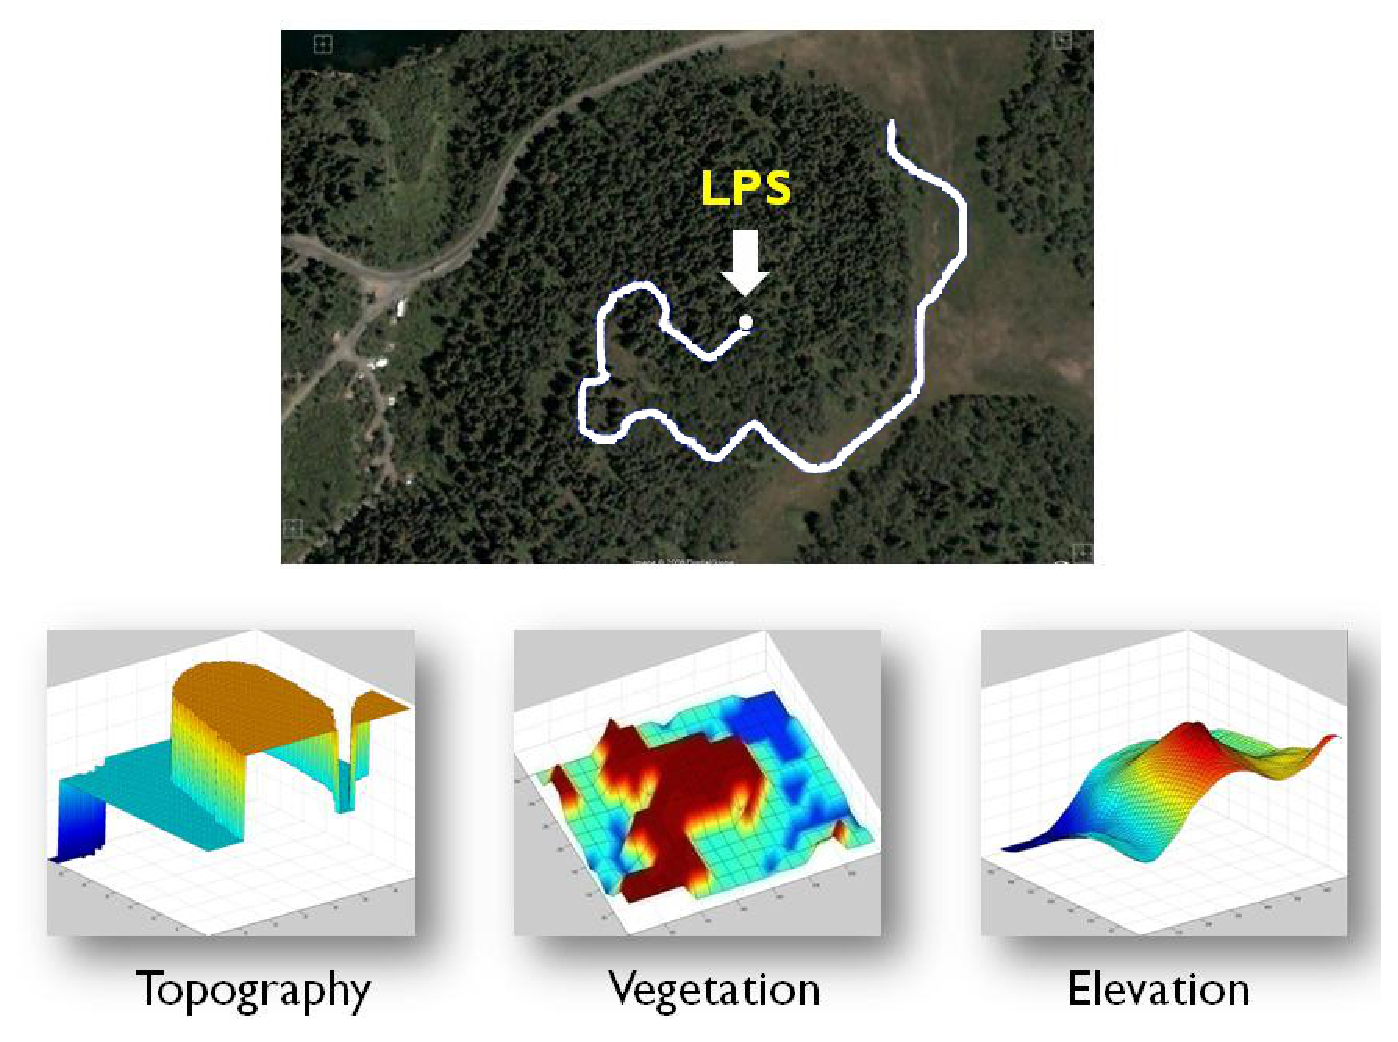
\includegraphics[width=5in]{satellite.eps}
\caption[Satellite imagery and terrain data of area by Payson Lake, Utah]{Satellite imagery of area by Payson Lake, Utah together with relative topography, vegetation, and elevation data downloaded from USGS web site. The topography and vegetation plots are discretized into (lake, plain, hill), and (sparse, medium, dense) respectively.}
\label{satellite}
\end{figure}

%---------------------------------------------------
\subsection{Hexagonal Tessellation Discretization}
\label{sec:3.3}

The first step in the model is to discretize the area into a hexagonal tessellation as shown in Figure~\ref{hexgrid}. The reason we use a hex tessellation is because the hex tessellation ensures the distance from the center of one cell to the center of any neighboring cell is always the same. The width of each hex cell is 24 meters. We picked this number because we believe such a granularity allows us to have enough detailed information about the terrain features without going into excessive details to burden the amount of computation. Future work should systematically explore how changing this granularity affects the tradeoffs between computational complexity and precision. In a real WiSAR scenario, the width can also be determined by the level of detail available for the terrain feature data at hand.

\begin{figure}
\centering
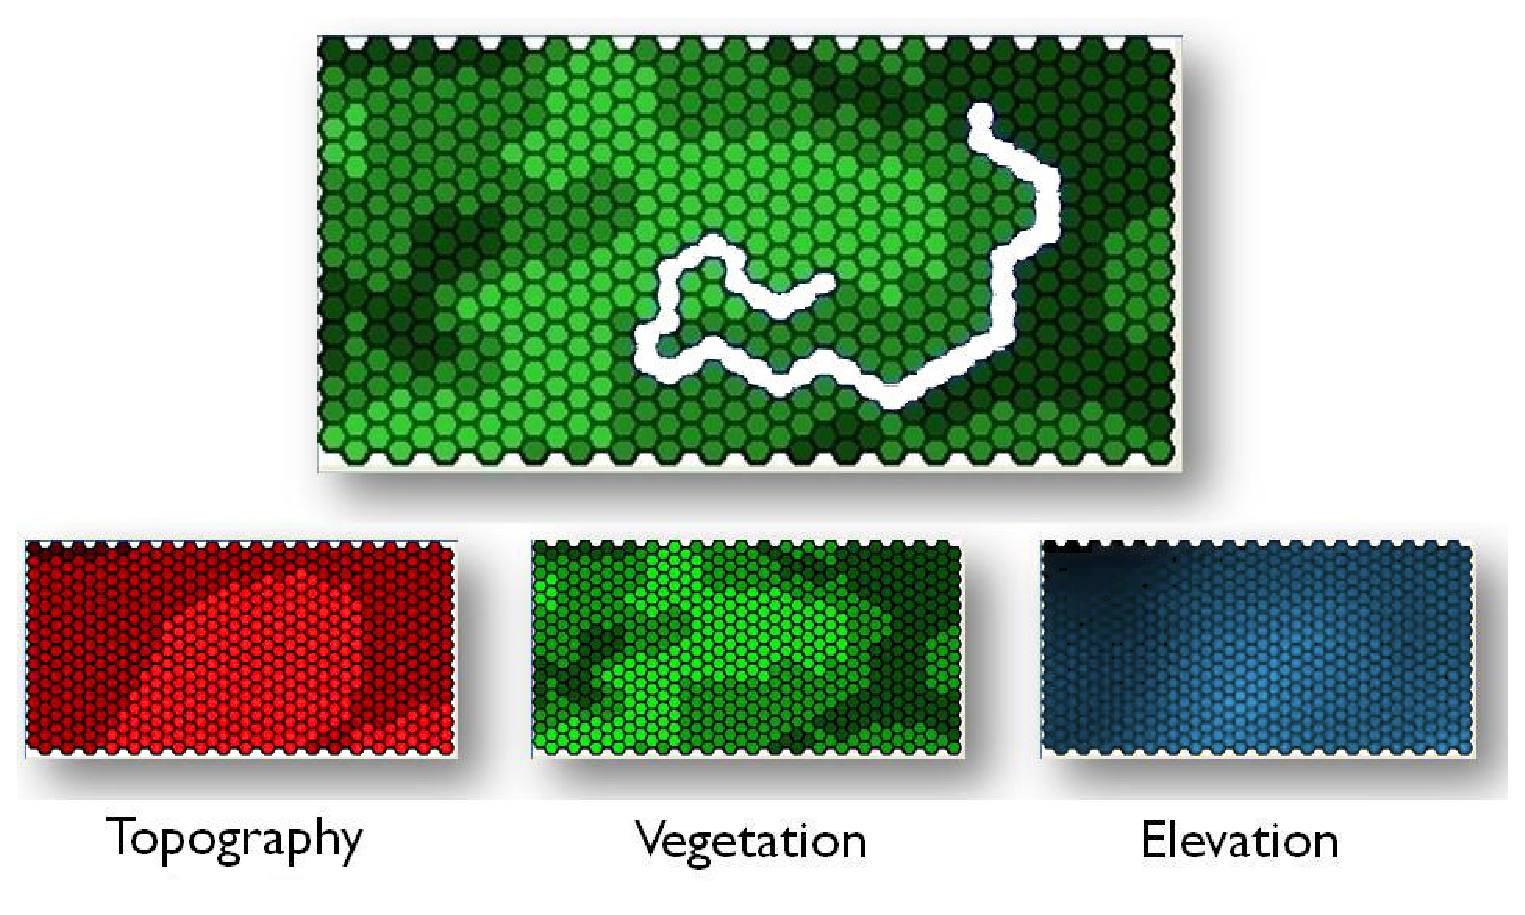
\includegraphics[width=5.5in]{hexgrid.eps}
\caption[Hexagonal discretized tessellation showing past historical data]{Hexagonal discretized tessellation showing past historical data (the path marked by the white cells in the main image) together with topography, vegetation, and elevation information in hexagonal tessellation.}
\label{hexgrid}
\end{figure}

The resulting tessellation is a $16 \times 38$ tessellation with 608 distinct states. Using the terrain feature data we have, each state is really a 3-tuple of (topography type, vegetation type, elevation). When we transition from one state to another neighboring state (including remaining in the same state), we can identify whether the topography type and vegetation type change. By calculating the elevation difference between the two states, we can find out whether the local slope is going uphill, downhill, or neither. Here we decide whether there is a local slope by calculating the angle of the elevation difference. If the difference is more than 20 degrees, we mark it as a local slope. We subjectively picked the threshold of 20 because we want to emphasize the extra effort of going uphill (as might be representative of a typical missing person such as a 14-year-old scout). Future work should systematically evaluate the impact of this threshold on usefulness of the probability distribution function.

%---------------------------------------------------
\subsection{Model Representation}
\label{sec:3.4}

In this sub-section, we define the Bayesian model in terms of the prior, the state transition, and the likelihood, and discuss each component in detail.

%*****************************
\subsubsection{The Prior}
\label{sec:3.4.1}

With the knowledge of past WiSAR incidents and expert opinion on human behavior, we can ask domain experts to specify their prior beliefs on how the missing person would behave with respect to different terrain features (e.g., a transition from a medium vegetation type to a dense vegetation type). For example, since we have three different topography types, we need a $3 \times 3$ transition matrix as shown in Equation~(\ref{matrix}), representing the probability of transitioning from one topography type to another. The rows and columns are both indexed by the different topography types, and it is possible to remain in the same topography, yielding
\begin{equation}
\left[
\begin{array}{ccc}
T_{00}' & T_{01}' & T_{02}'\\
T_{10}' & T_{11}' & T_{12}'\\
T_{20}' & T_{21}' & T_{22}'\\
\end{array}
\right]
\label{matrix}
\end{equation}
For example, $T_{00}'$ is the transitional probability for remaining in the lake type topography, and $T_{00}'$ is a number between 0 and 1 inclusive. The definition of the transition matrix requires that the values in each row of the matrix sum up to 1.

However, we would also like to enable the domain experts to incorporate uncertainty in their beliefs. Therefore, for each topography transition, instead of a number, a continuous Beta distribution is used, and a probability value, such as $T_{00}'$, can be generated by sampling from the Beta distribution. We use a Beta distribution because the domain of a Beta distribution's probability density function is $x \in [0; 1]$, which matches the parameter space of probability values. The curves of the Beta distribution also have the shape we desire because the mean and the mode of the curve can shift between 0 and 1 with various variances depending on what parameters we pick (illustrated in Figure~\ref{BetaPDF}). To specify uncertainty, for each topography transition probability, we ask the domain experts to provide a mean and a variance because these parameters are much easier to understand for non-statisticians compared to the $\alpha$ and $\beta$ parameters for the Beta distribution. Then we solve for the $\alpha$ and $\beta$ parameters automatically.

\begin{figure}
\centering
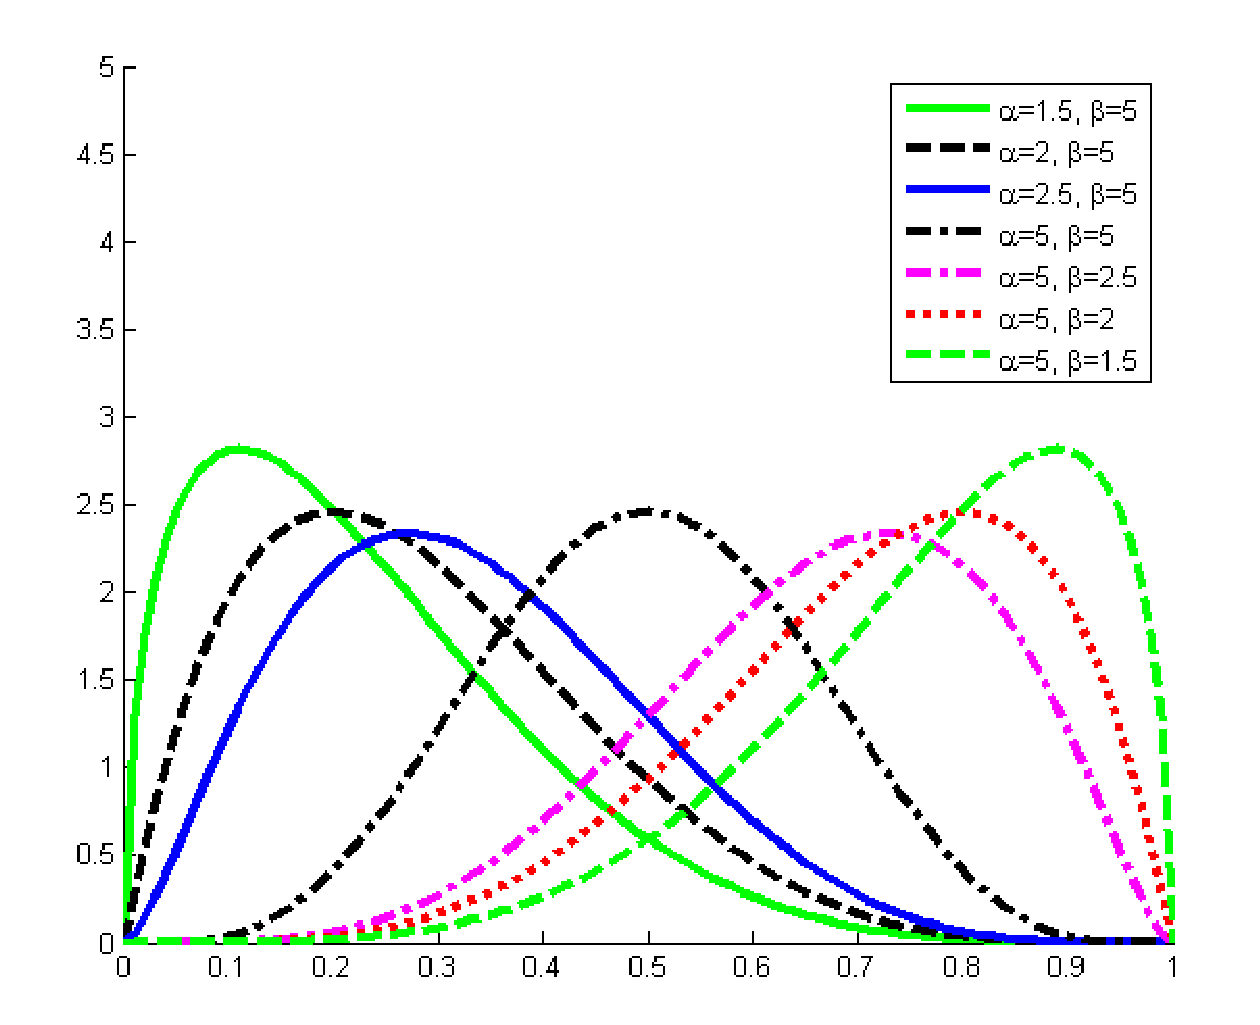
\includegraphics[width=5in]{BetaPDF.eps}
\caption[Beta Distribution probability density function]{Beta Distribution probability density function}
\label{BetaPDF}
\end{figure}

We have to be careful here to make sure the transition matrix, shown in Equation~(\ref{matrix}), is still valid. For example, the domain experts can specify means for Beta distributions relating to transitioning from topography type ``plain'' to all three topography types as 0.5, 0.3, and 0.2. These numbers sum up to 1. Unfortunately when we sample from the three Beta distributions, the values we get could possibly be something like 0.5, 0.35, and 0.22, which do not sum up to 1. That means these numbers are not true probability values, and we have to normalize them so they become true probability values. Therefore, we use $T_{ij}$ to denote the value we generate from the Beta distribution corresponding to transitioning from topography feature $i$ to topography feature $j$, and use $T_{ij}'$ to denote the true probability value (after normalization) for the transition. The probability distributions of $T_{ij}$ are the domain experts' prior beliefs with respect to topography terrain features, and there are 9 of them.

Similarly, since we have three different vegetation density types, we also need a $3 \times 3$ transition matrix to represent the probability of transitioning from one vegetation density type to another. This adds 9 vegetation density related priors to the model. With respect to local slopes, since there are only three possible transitions (uphill, no slope, and downhill), there are only 3 more priors to specify.

Therefore, our model has a total of 21 priors (9 related to topography, 9 related to vegetation density, and 3 related to local slope). For simplicity, we denote the joint distribution of all the priors as $\pi(\underline{\theta})$, where 
\begin{align}
\label{21}
\underline{\theta} &=T_{00},T_{01},...,T_{22},V_{00},V_{01},...,V_{22},S_0,S_1,S_2
\end{align}
and each prior follows a Beta distribution with known $\alpha$ and $\beta$ values (solved using the mean and variance values provided by domain experts). Thus
\begin{align}
\label{BetaT}
T_{ij} \sim Beta(\alpha_{T_{ij}}, \beta_{T_{ij}})\\
\label{BetaV}
V_{ij} \sim Beta(\alpha_{V_{ij}}, \beta_{V_{ij}})\\
\label{BetaS}
S_{i} \sim Beta(\alpha_{S_{i}}, \beta_{S_{i}})
\end{align}
where $T_{ij}$ represents the probability of transitioning from topography type $i$ to $j$ (possibly $i=j$) where $i=0,1,2$ and $j=0,1,2$. Similarly, $V_{ij}$ represents the probability of transitioning from vegetation type $i$ to $j$, and $S_{i}$ represents the probability of following a certain local slope type $i$.

%*****************************
\subsubsection{State Transition}
\label{sec:3.4.2}

In an earlier part of the paper we described how the search area is discretized into a hexagonal tessellation. Each cell becomes a state. Let $X$ represent a state, then $X$ can be defined as a vector containing information about the hexagonal cell:\\

\indent{}$X$ = [topography, vegetation density, elevation, index of tessellation]\\

With our model, we assume the state transition follows a first-order Markov process, meaning that the next state the lost-person (LP) will be in is only dependent on the current state the LP is in.
\begin{align}
\label{FirstOrder}
P(X_t|X_0, X_1, ..., X_{t-1}) = P(X_t|X_{t-1})
\end{align}

This is a strong assumption and it might not hold. For example, the amount of time traveled following the same direction (e.g., 20 minutes) could affect whether the LP wants to turn around and backtrack; similarly, the intended destination might affect which path the LP chooses while looking for the way. However, we argue that because the LP is in a disoriented state (although the LP might think otherwise) in the wilderness, the direction the LP follows could very well not be the direction the LP thinks he/she is following. Therefore, this assumption should not prevent the model from having useful predictive power. However, we also plan to extend the model in future work that will take into consideration the intended destination and incorporate that information into the representation of the current state.

When we compute $P(X_t|X_{t-1})$, it is necessary to combine the topography transition probability with vegetation density and local slope so we can borrow strength from each of the terrain features. We denote $T(Y|X)$ as the probability of transitioning from the topography of state $X$ to the topography of state $Y$, and $V(Y|X)$ as the probability of transitioning from the vegetation density type of state $X$ to the vegetation density type of state $Y$. Using the elevation difference between state $X$ and state $Y$, we can identify the local slope of going from state $X$ to state $Y$. We denote $S(Y|X)$ as the probability of transitioning from state $X$ to state $Y$ only based on local slope information. $T(X|Y)$, $V(X|Y)$, and $S(X|Y)$ are all true probability values, and they correspond to the relevant entries in the terrain features transition matrices such as Equation~(\ref{matrix}). Assuming the three terrain features are independent of each other we can combine the three probabilities by taking the product of the three,
\begin{align}
\label{product}
P(X_t|X_{t-1}) \propto T(X_t|X_{t-1})V(X_t|X_{t-1})S(X_t|X_{t-1}),
\end{align}
where $P(X_t|X_{t-1})$ is the entry in the row indexed by $X_t$ and the column indexed by $X_{t-1}$ in the state transition matrix describing the probability of transitioning from any state to any other state (including transitioning into the same state). Here $P(X_t|X_{t-1})$ is a true probability value.

Because a person can only travel from one hexagonal cell to its neighboring cells (or remain in the original cell), in each row of the state transition matrix, the transitional probabilities for all $X_t \notin N(X_{t-1})$ will be 0, where $N(X_{t-1})$ is the set of neighboring states of state $X_{t-1}$ (including $X_{t-1}$). That means the sum of $P(X_t|X_{t-1})$ for all $X_t \in N(X_{t-1})$ is 1 (elements in each row of the state transition matrix should sum to 1). 

If we look at each hex cell closely, we can see that from each cell a person can travel to one of the six neighboring cells or remain in the same cell. 
\begin{align}
\label{sub}
\mathrm{Let}~\underline{\phi'} &= P(X_t|X_{t-1}) ~\mathrm{where}~ X_t \in N(X_{t-1})\\
\mathrm{Let}~\underline{\phi} &= T(X_t|X_{t-1})V(X_t|X_{t-1})S(X_t|X_{t-1}) ~\mathrm{where}~ X_t \in N(X_{t-1})
\end{align}

We know $\underline{\phi}$ and $\underline{\phi'}$ each have 7 elements, and $\sum_{i=1}^7 \phi_i' = 1$, where
\begin{align}
\label{phi}
\phi_i' = \dfrac{\phi_i}{\sum_{j=1}^7 \phi_j}
\end{align}

Equation~(\ref{phi}) normalizes the products of terrain feature transition probabilities to compute the $P(X_t|X_{t-1})$ entries for all neighbors of state $X_{t-1}$.

%*****************************
\subsubsection{The Likelihood}
\label{sec:3.4.3}

Because from each cell a person can travel to one of the six neighboring cells or remain in the same cell, the likelihood of one observation (how the lost person traveled from one cell to one of the neighboring cells), denoted as $f(z|\underline{\theta})$, follows a categorical distribution with 7 dimensions. Relating to the previous section, $z$ can be defined as
\begin{align}
z = (X_t, X_{t-1}), ~\mathrm{where}~ X_t \in N(X_{t-1}).
\end{align}
In other words, $z$ is really a vector in the form of a 7-tuple, but to avoid notation confusion, we will only use $\underline{z}$ to denote multiple observations in a later section when we discuss posteriors. If we use $z_i$ to represent each element in vector $z$, then $z_i$ is constrained by
\begin{align}
\label{}
z_i \in \{0,1\} ~\mathrm{and}~ \sum_{i=1}^7 z_i=1,
\end{align}
meaning exactly one element in the 7-tuple is 1 and the others are all 0s. For example, an observation can be of the form of (0,0,0,0,1,0,0), meaning the person traveled to the fifth neighboring cell. Thus, our observation given all the prior beliefs is governed by
\begin{align}
\label{CAT}
z|\underline{\theta} &\sim CAT(\underline{\phi'}), ~\mathrm{where}\\
\underline{\phi'} &= \phi_1', \phi_2', ..., \phi_7', ~\mathrm{and}\\
%\end{align}
%\begin{align}
\label{likelihood}
f(z|\underline{\theta}) &= \prod_{i=1}^7 \phi_i'^{z_i},~\mathrm{where}\\
\underline{\theta} &= T_{00},T_{01},...,T_{22},V_{00},V_{01},...,V_{22},S_0,S_1,S_2.
\end{align}

Note that in order to compute the likelihood for $z$ using Equation~(\ref{likelihood}), we need to identify $X_{t-1}$, the state the person is in, and all neighboring states $X_t \in N(X_{t-1})$. We also need to sample from our priors $\pi(\underline{\theta})$ in order to construct terrain features transition matrices, which are then used in Equations~(\ref{sub}) --~(\ref{phi}) to compute $\underline{\phi'}$.

Figure~\ref{BN} illustrates the process of computing the likelihood graphically. The top row shows the 21 priors we sample from to generate $\underline{\theta}$ (9 for topography, 9 for vegetation density, and 3 for local slope). After normalization, we obtain all the entries for the terrain features transition matrices as shown in the second row (9 priors from the $3 \times 3$ topography transition matrix: $T_{00}', T_{01}', ..., T_{22}'$, 9 from the $3 \times 3$ vegetation density transition matrix: $V_{00}', V_{01}', ..., V_{22}'$, and 3 local slope probabilities: $S_0, S_1, S_2$). Depending on the $X_{t-1}$ and $X_{t}$ states associated with $z$, relevant $T(X_t|X_{t-1})$, $V(X_t|X_{t-1})$, and $S(X_t|X_{t-1})$ probability values are identified and multiplied to compute $\underline{\phi}$ (third row). The elements of the $\underline{\phi}$ vector are further normalized to produce $\underline{\phi'}$ (fourth row), which are the probabilities of the lost person traveling from state $X_{t-1}$ to all the neighboring states.

\begin{figure}
\centering
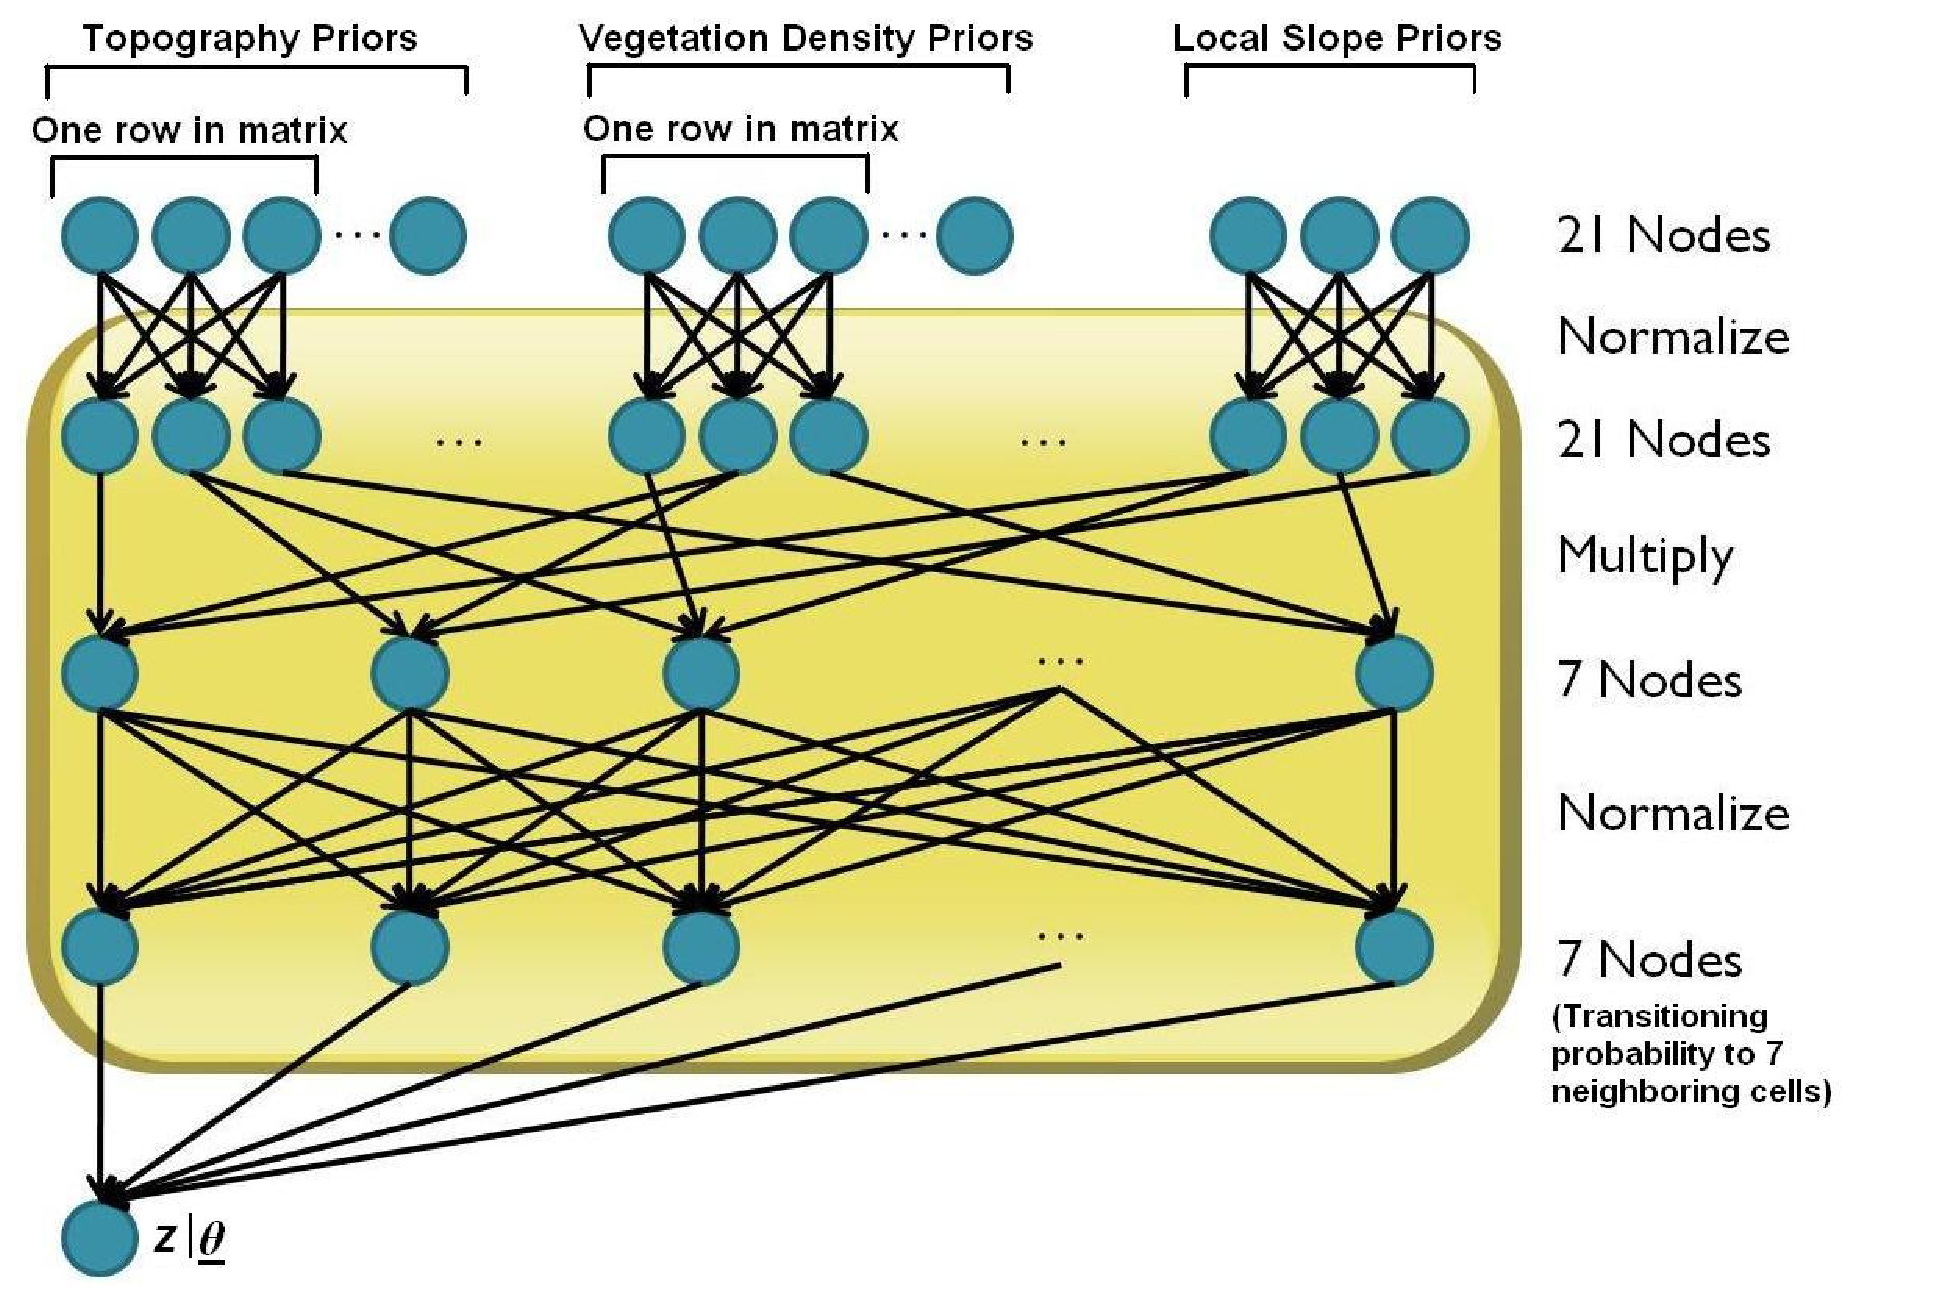
\includegraphics[width=6in]{BN.eps}
\caption{A graphical illustration of the proposed model. Top row: probability distribution for each prior belief. Fourth row: probability of transitioning into a neighboring cell in the hex tessellation. Bottom row: an observation indicating possible travel directions for the lost person.}
\label{BN}
\end{figure}

Once samples are generated from the priors $\pi(\underline{\theta})$, we can deterministically compute the values for the middle layers --- they are simply delta functions. Therefore, when we build the Bayesian network to compute the posteriors, we collapse all the middle layers and only keep the top and bottom layers.

%---------------------------------------------------
\subsection{Using the Model to Compute the Posterior}
\label{sec:3.5}

A great benefit of using a Bayesian model is that we can incorporate existing observations to update prior beliefs. The updated beliefs are the posterior beliefs.

Existing observations in the model are in the form of sections of GPS track logs (also discretized to a hexagonal tessellation) together with the terrain features associated with the track logs. By combining existing human behavior data with prior beliefs, we can reduce the domain experts' uncertainty.

To incorporate multiple observations, we simply add multiple $z|\underline{\theta}$ nodes in the bottom row of the Bayesian network (illustrated in Figure~\ref{BNPost}). The network is dynamically built with appropriate parent nodes identified and linked to the observation nodes dynamically.
\begin{figure}
\centering
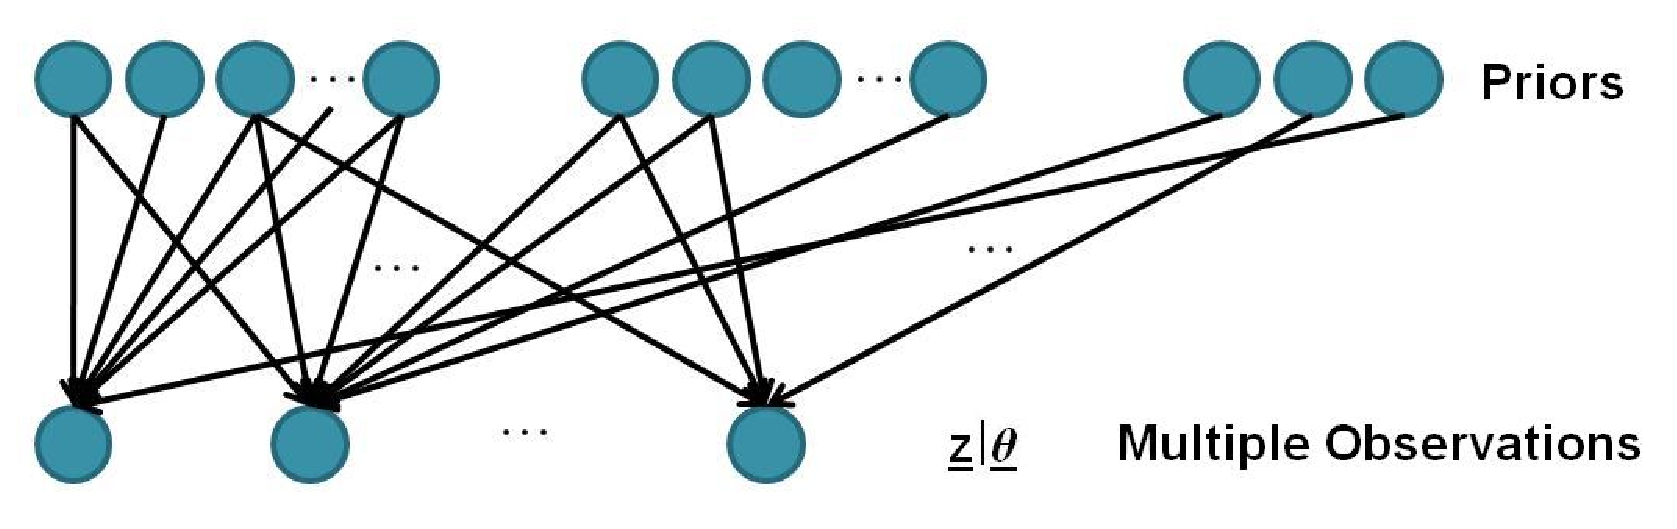
\includegraphics[width=6in]{BNPost.eps}
\caption{Bayesian network with multiple observations. Top row: probability distribution for each prior belief. Bottom row: multiple observations from previously collected human behavior data in the form of segments of GPS track logs together with terrain features associated with the track logs.}
\label{BNPost}
\end{figure}

Because of the complexity of the model, it is impossible to solve for the posterior distribution $\pi(\underline{\theta}|\underline{z})$ in closed form. That is why we used an MCMC approximation algorithm as the generation tool. Specifically, we used a random walk flavor of MCMC that uses the Gibbs Sampling algorithm, shown in~\cite{Gelman2004Bayesian}, on the outside loop, with Metropolis-Hastings algorithm, shown in~\cite{Gelman2004Bayesian}, inside each iteration of the Gibbs Sampling. Gibbs sampling is an algorithm for generating samples from a joint probability distribution of multiple random variables when the conditional distribution of each variable is known. It generates samples from the distribution of each variable in turn, conditioned on the current values of other variables. The Metropolis-Hastings algorithm generates a first-order Markov chain in each state and uses a proposal density, which depends on the current state, to generate a new proposed sample. This value is accepted if a value drawn from a uniform distribution between 0 and 1 meets certain requirements. Otherwise, the current value is retained. In our implementation, we used a Gaussian function as the proposal density.

In our implementation, we used 500 iterations for burn (throwaways) and kept 10,000 samples for each parent node. In each iteration, the Gibbs Sampling algorithm tries to sample from the distribution of each parent node in turn, conditioned on the current values of other parent nodes. However, Gibbs Sampling relies on the Metropolis-Hastings algorithm to really generate samples from the posterior distribution by using a proposal density function (a Gaussian distribution in our case). These samples approximate the posterior distribution for each of our 21 priors. 

Figure~\ref{Approximation} illustrates how the Monte Carlo method approximates the posterior distribution of one parameter (a parent node). In each iteration, the Metropolis-Hastings algorithm probabilistically generates a sample for the node based on the complete conditional constructed by Gibbs sampling (points inside smaller graphs in the upper portion where each point represents a probability value generated from a Beta distribution). If we combine all these samples into one graph and bin the points into small clusters (bigger graph in lower portion where the y axis is the count), we can connect the top of the bins and draw a curve. This curve is an approximation of the posterior distribution of the node, and as the number of samples approaches infinity, the curve matches the actual posterior distribution.

\begin{figure}
\centering
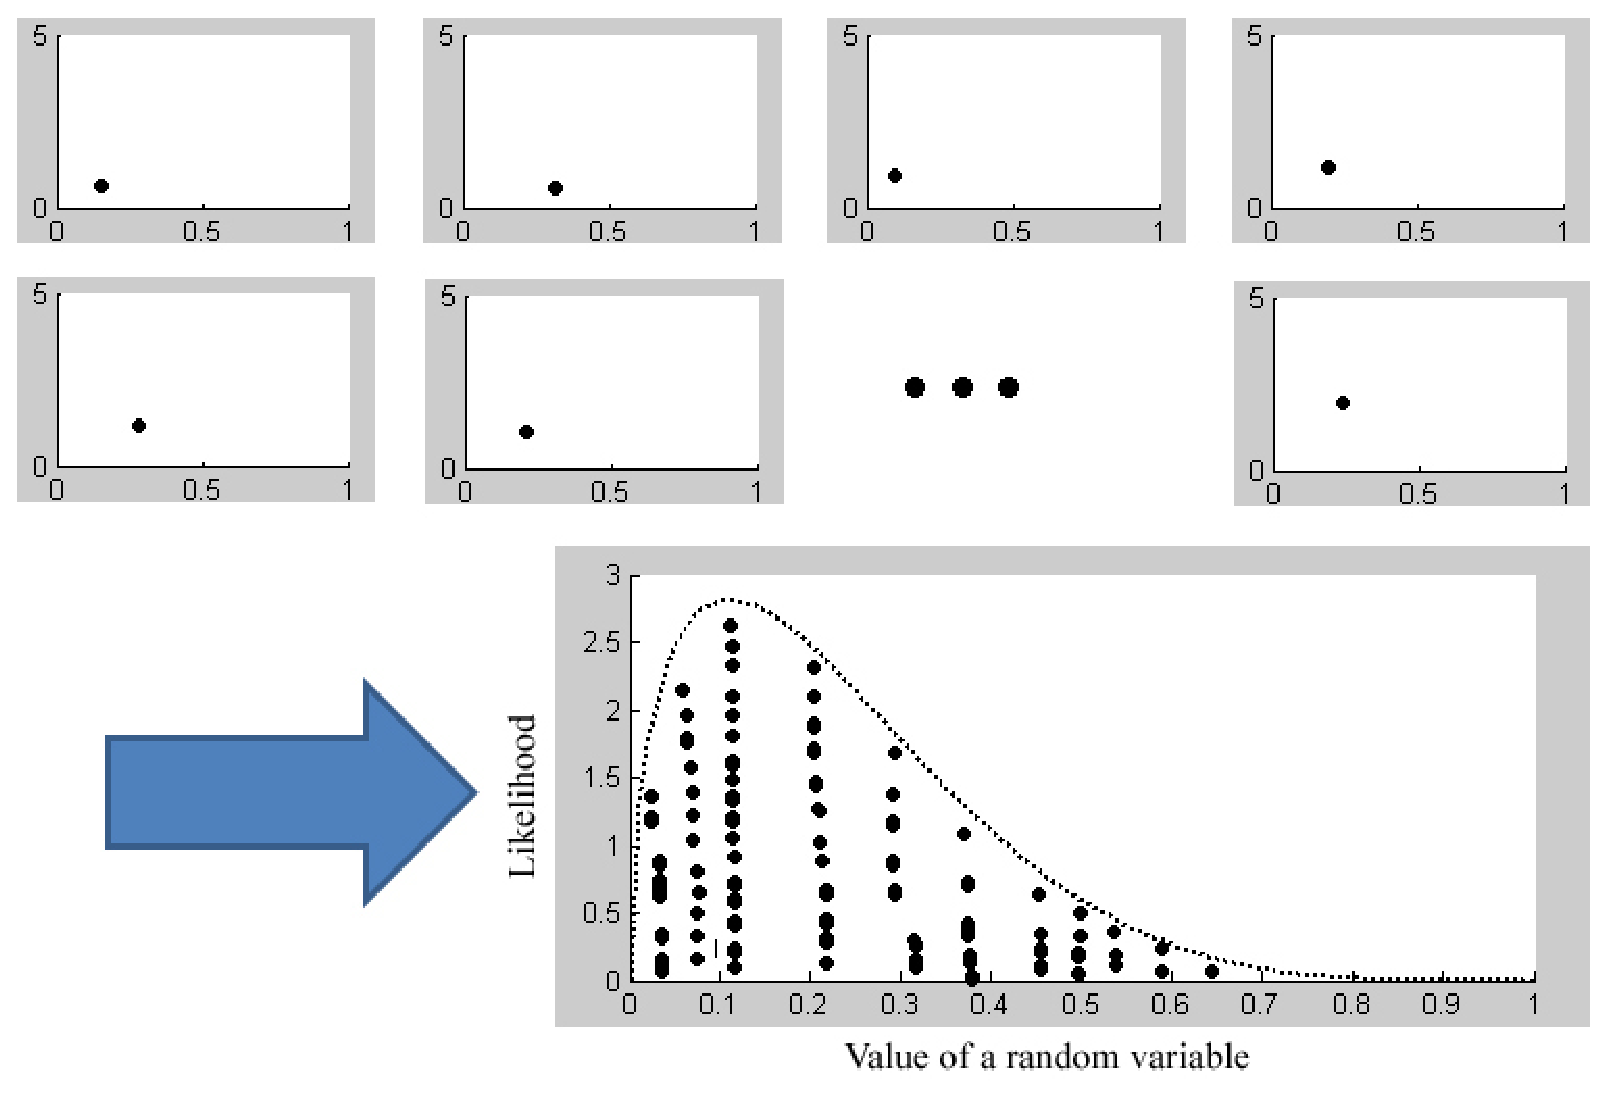
\includegraphics[width=5.5in]{Approximation.eps}
\caption{Graphical illustration of how the Monte Carlo method approximates the posterior distribution of one parameter. Upper: multiple iterations of sampling. Lower: samples clustered to approximate the real distribution.}
\label{Approximation}
\end{figure}

In our experiments, the MCMC algorithm completed in 220~seconds on a Dual-core AMD 3800+ PC with 3GB of memory.

%---------------------------------------------------
\subsection{Using the Model to Compute the Predictive Probability Distribution}
\label{sec:3.6}

Using the model described above, once we have the priors specified, we can build our $608 \times 608$ state transition matrix. In our implementation, we sample once from each Beta distribution for each time step. Starting from the lost person's point last seen, we can generate the prior predictive probability distribution by multiplying the state transition matrix in each time interval. This method allows the search and rescuers to see how the predictive probability distribution changes as time progresses.

~\cite{Setnicka1980Wilderness} and~\cite{Syrotuck2000Introduction} show that in WiSAR scenarios, as time progresses, the effective search radius increases by approximately 3km/hour, which is equivalent to 50m/minute. Because the age of the lost-person affects the speed the person travels, we can adjust the size of the time interval accordingly. With our lost scout scenario, because children generally travel slower than adults, we assume the lost scout travels at roughly 24m/minute; therefore, we define each time step as 1 minute. When we multiply the state transition matrix (sampled once from the prior distributions at each time step) 200 times (3 hours and 20 minutes = 200 minutes), we have the prior predictive probability distribution map as shown in the upper row of Figure~\ref{priorvspost}.

Once we combine previously collected human behavior data and approximate the joint posterior distribution of all the parameters, we can sample from the posterior beliefs instead of the prior beliefs. Following the same state transition matrix multiplication, we can also generate the posterior predictive probability distribution. The lower row of Figure~\ref{priorvspost} shows this distribution. In the Wilderness Search and Rescue case, the posterior predictive probability distribution is the 2D probability distribution map we are seeking.

\begin{figure}
\centering
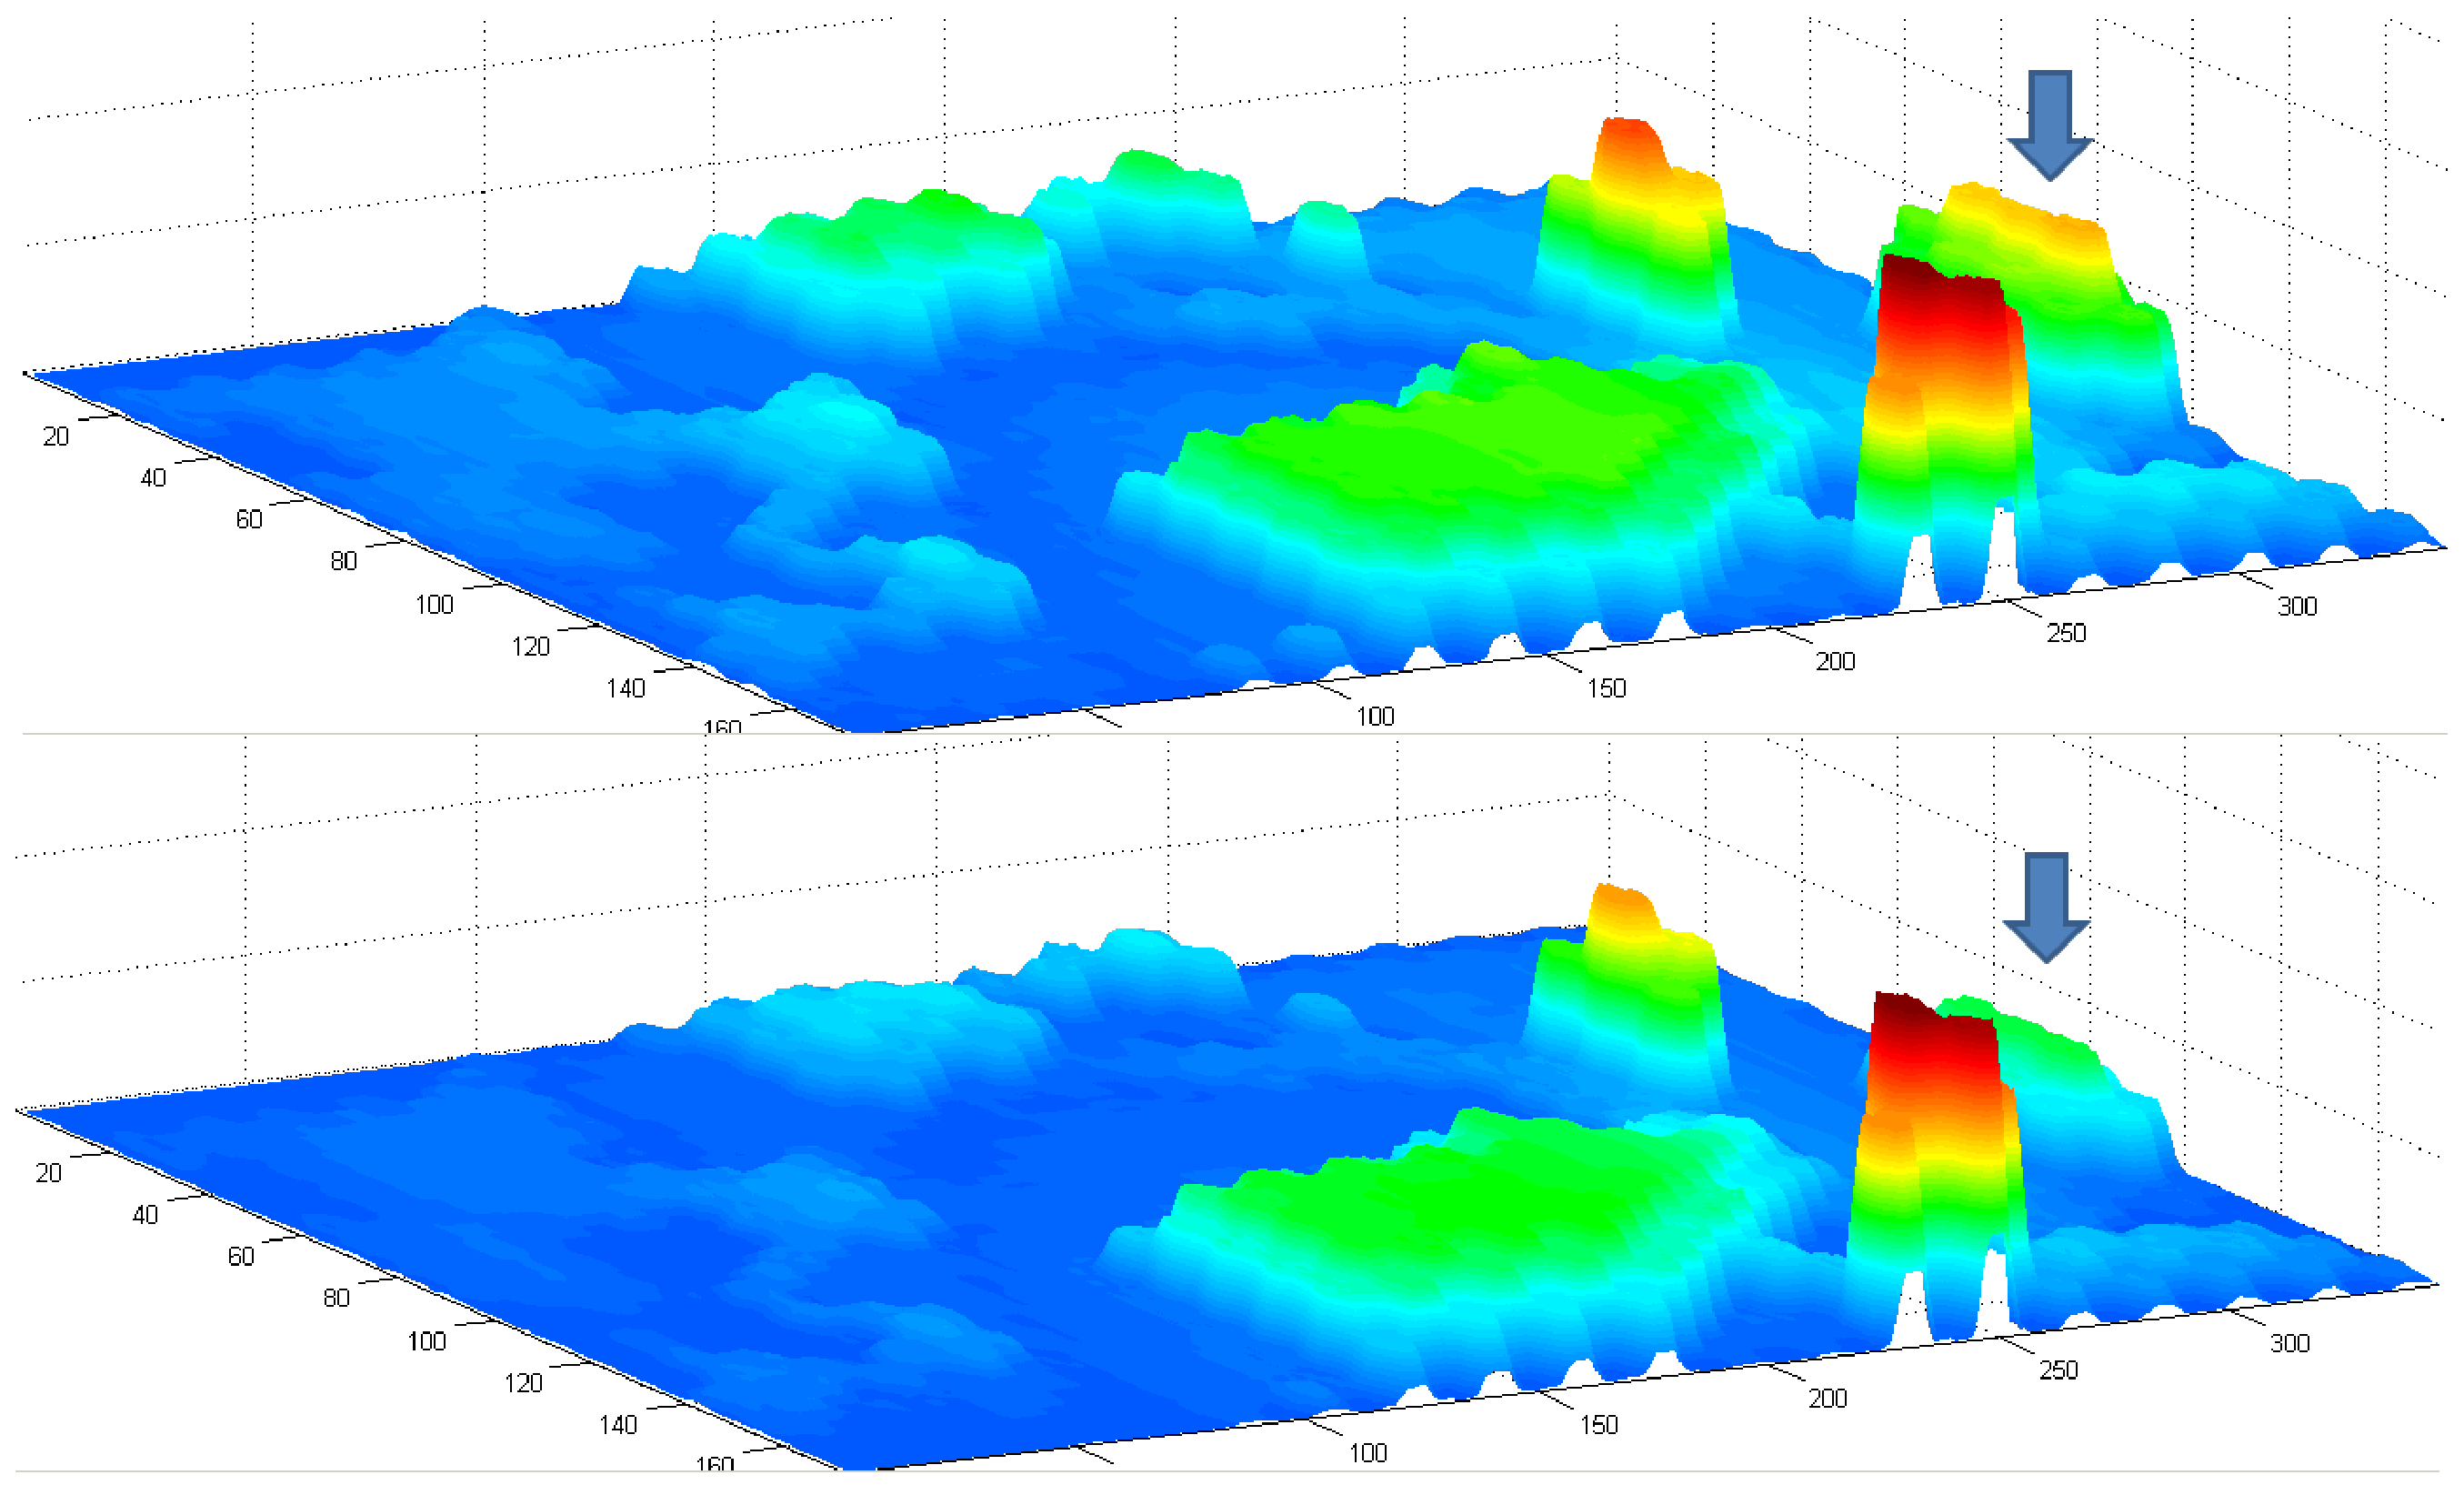
\includegraphics[width=6in]{priorvspost.eps}
\caption[Comparing prior predictive distribution against posterior predictive distribution]{Comparing prior predictive distribution (upper row) against posterior predictive distribution (lower row)}
\label{priorvspost}
\end{figure}

%=====================================================================================================
\section{Evaluation of the Model}
\label{sec:4}

%---------------------------------------------------
\subsection{Synthetic Data}
\label{sec:4.1}

Pretending to be domain experts, we specified all the prior distributions by setting the means and the variances. The matrices below show the prior distributions we set for the vegetation type transition matrix. The first matrix shows the means and the second matrix shows the variances.
\begin{equation}
\centering
\left[
\begin{array}{ccc}
\mu_{V_{00}}=0.6 & \mu_{V_{01}}=0.25 & \mu_{V_{02}}=0.15  \\
\mu_{V_{10}}=0.5 & \mu_{V_{11}}=0.3 & \mu_{V_{12}}=0.2  \\
\mu_{V_{20}}=0.4 & \mu_{V_{21}}=0.4 & \mu_{V_{22}}=0.2  \\
\end{array}
\right]
\end{equation}
\begin{equation}
\centering
\left[
\begin{array}{ccc}
\sigma^2_{V_{00}}=0.14^2 & \sigma^2_{V_{01}}=0.15^2 & \sigma^2_{V_{02}}=0.1^2 \\
\sigma^2_{V_{10}}=0.15^2 & \sigma^2_{V_{11}}=0.15^2 & \sigma^2_{V_{12}}=0.15^2 \\
\sigma^2_{V_{20}}=0.15^2 & \sigma^2_{V_{21}}=0.15^2 & \sigma^2_{V_{22}}=0.15^2 \\
\end{array}
\right]
\end{equation}

We set these values following common sense. For example, we believe a lost scout is more likely to remain in sparse vegetation type ($\mu_{V_{00}}=0.6$) and unlikely to transition from a sparse vegetation type to a dense vegetation type ($\mu_{V_{02}}=0.15$). We also believe a lost scout is more likely to transition from a dense vegetation type to a medium or sparse vegetation type and from a medium vegetation type to a sparse vegetation type ($\mu_{V_{21}}=0.4$, $\mu_{V_{20}}=0.4$, $\mu_{V_{10}}=0.5$). However, for most of these Beta distributions, we are not certain about our estimation, which is why we specified large variances for most of the parameters. For example, $\sigma^2_{V_{10}}=0.15^2$ means we believe the probability to transition from vegetation type medium to sparse could be as low as 0.05 and as high as 0.95. In real WiSAR scenarios, the priors should come from past statistical analysis of lost-person behaviors, such as~\cite{Heth1998Characteristics} and~\cite{Syrotuck2000Analysis}, combined with domain experts' opinions.

Each observed data point is a transition from one cell to another neighboring cell (including remaining in the same cell) in previously collected GPS track logs. The track logs do not even have to be in the same search area of the current incident. What we really care about is how terrain features affect a person's behavior in the wilderness. If the track logs contain this kind of information, we can use it to update our prior beliefs. These posterior beliefs can then be used in a generative approach to predict how the lost person might travel from the point last seen as time progresses. For the lost scout scenario, our observed data is partly shown in Figure~\ref{hexgrid} as the path of white cells. We use the word ``partly'' because during the travel, the person sometimes stayed in the same state during the 1-minute time interval. To test the robustness of the model, we intentionally designed the data set so that the person remained in the same vegetation type most of the time. We also repeated the same path three times in our synthetic dataset to simulate three different past GPS track logs. By repeating these we are basically adding more strength to the data and we expect the data to have a much stronger effect on the posterior distributions for the parameters. Each path consists of 45 transitions; therefore, our dataset has 135 data points.



%We are currently in the process of collecting real human behavior data in the form of GPS track logs from hikers\footnote{http://alltrails.com/}, hunters, and geocachers\footnote{http://tanglefoot.cs.byu.edu/~amy/index.html}. Note that historical datasets from different areas can be used together to generate posterior distributions for the same set of parameters, but samples generated from the posterior distributions will be used on the same search area in order to generate predictive distributions.

%---------------------------------------------------
\subsection{Prior vs. Marginal Posterior}
\label{sec:4.2}

Using the posterior samples, we can compare the marginal prior distribution with the marginal posterior distribution for each of our parameters. Figure~\ref{posts} shows the comparison for some of the parameters. The dotted lines represent the prior distributions and the solid lines represent the posterior distributions.

The plot in the upper left is for parameter $T_{02}$, the terrain feature transition probability from lake to hill. Since we do not have any data point in our dataset that transitioned from lake to hill, here we see the posterior is almost identical to the prior. The plot in the upper right is for parameter $T_{12}$, the terrain feature transition probability from plain to hill. In our dataset, a good segment of the path basically followed the contour line but stayed in the plain states. This characteristic of the dataset explains why the posterior distribution is much narrower and had a much lower mean---because the data did not show many changes from plain to hills, the posterior probability of this transition is much lower with less variance. The plot in the lower left is for parameter $V_{01}$, the terrain feature transition probability from vegetation type sparse to medium. The plot in the lower right is for parameter $S_1$, the terrain feature transition probability from no slope to no slope. Both of these posteriors are only slightly different from the priors.
\begin{figure}
\centering
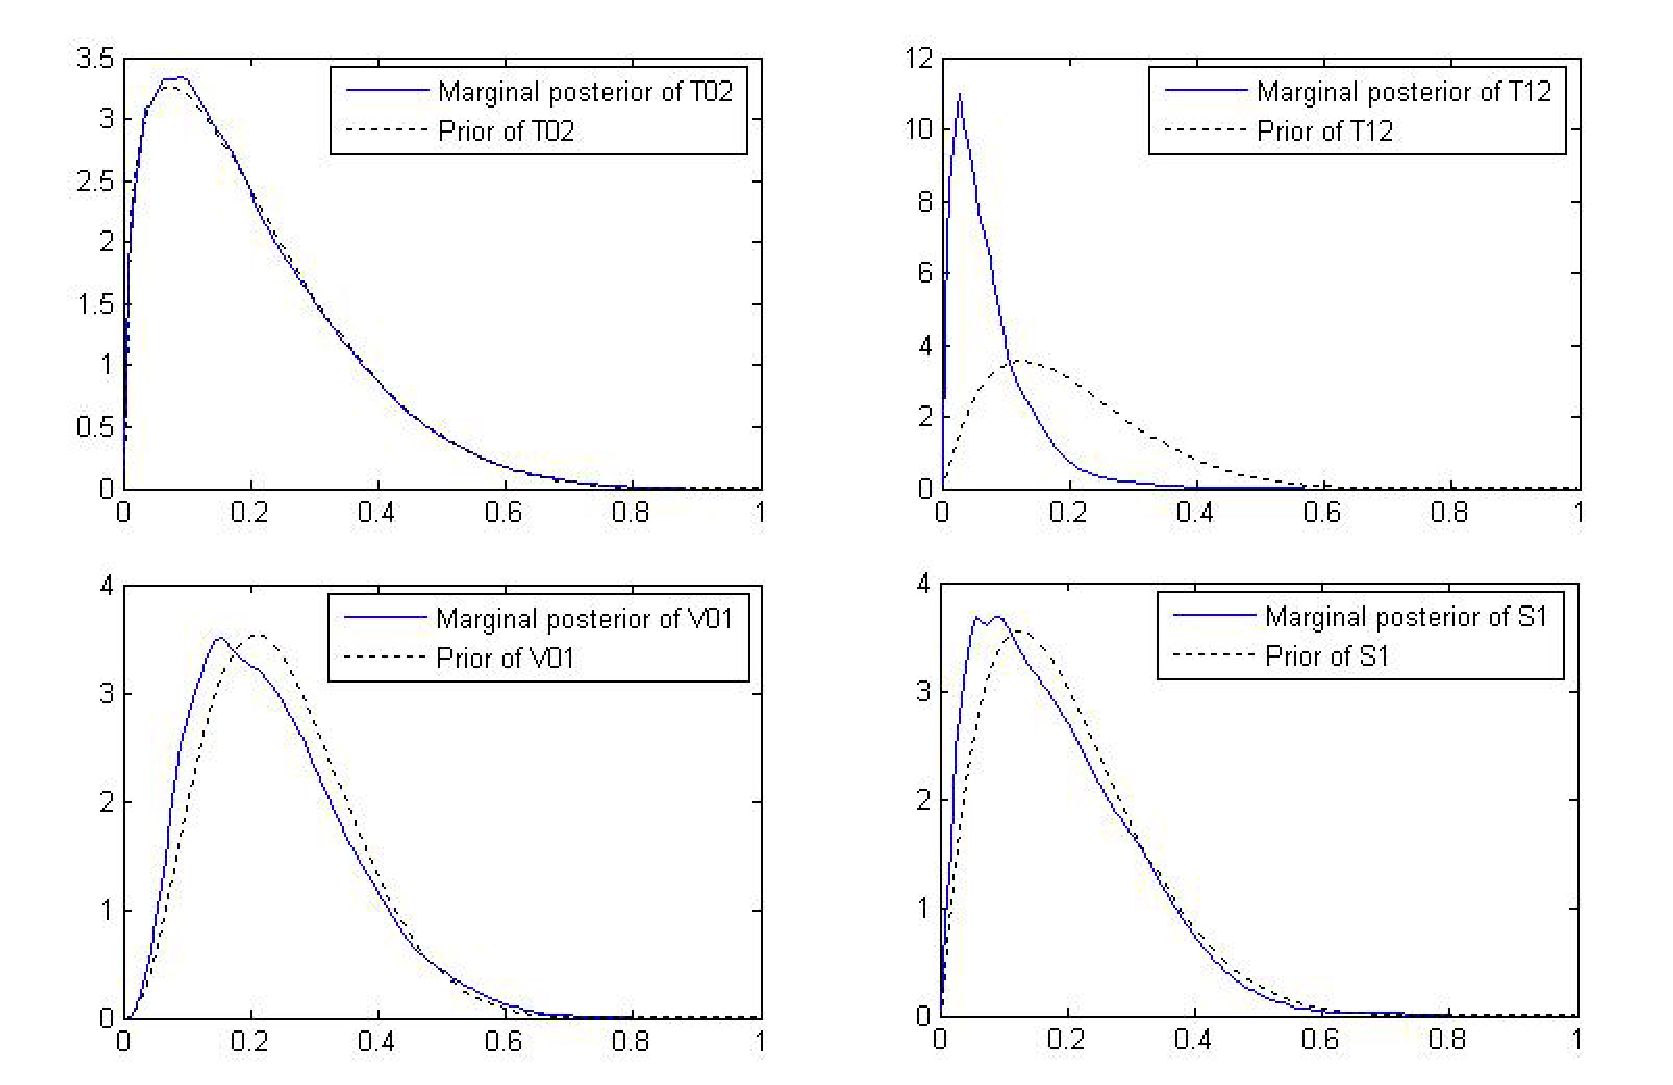
\includegraphics[width=6in]{posts.eps}
\caption[Comparing prior distribution with marginal posterior distribution]{Comparing prior distribution with marginal posterior distribution. Upper Left: $T_{02}$ Upper Right: $T_{12}$ Lower Left: $V_{01}$ Lower Right: $S_1$.}
\label{posts}
\end{figure}

%---------------------------------------------------
\subsection{Correlation of Parameters}
\label{sec:4.3}

When we ask the domain experts to specify the priors, we assume the parameters are independent. Because we have 21 parameters, the joint posterior distribution in the parameter space is really a distribution with 21 dimensions, which is impossible to plot. Instead, we use a correlation image to show whether there exist correlations between pairs of parameters.

Figure~\ref{correlation} shows a graphical representation of the correlation between each pair of parameters. A grey value, such as cell(1,21) in the lower left corner, indicates that there is no correlation between the two parameters. A white cell, such as cell(1,1) in the upper left corner, means the two parameters are fully positively correlated, and a black cell means the two parameters are fully negatively correlated. Here we see that the vegetation parameters $V_{20}$ (dense to sparse), $V_{21}$ (dense to medium), and $V_{22}$ (dense to dense) showed positive correlation. Other positive correlations also mostly appear between neighboring parameters. There is also a clear positive correlation between $V_{22}$ (Vegetation: dense to dense) and $S_{0}$ (uphill). These positive correlations are marked by the big circle in Figure~\ref{correlation}.

The results of the correlation analysis indicate that there is likely a correlation among different terrain features. Interestingly, from this figure we can see that parameter $V_{12}$ (Vegetation: medium to dense) and $T_{11}$ (Topography: plain to plain) are clearly, negatively correlated (marked by the upper small circle in Figure~\ref{correlation}). Parameter $V_{22}$ (Vegetation: dense to dense) and $T_{11}$ (Topography: plain to plain) are also clearly, negatively correlated (marked by the lower small circle in Figure~\ref{correlation}). A closer look at the terrain features of the area shows that dense vegetation is mostly located on the hill topography type and medium vegetation is mostly located on the plain topography type. This explains why we see such a negative correlation. This emergence of correlations that are compatible with terrain features suggests that the process of combining prior information with observed track logs is useful. However, when we let the domain experts specify the prior distributions, it is much more intuitive for them to assume independence instead of specifying conditional probabilities (to specify how the parameters are correlated), and we rely on data to identify the dependence relationship.
\begin{figure}
\centering
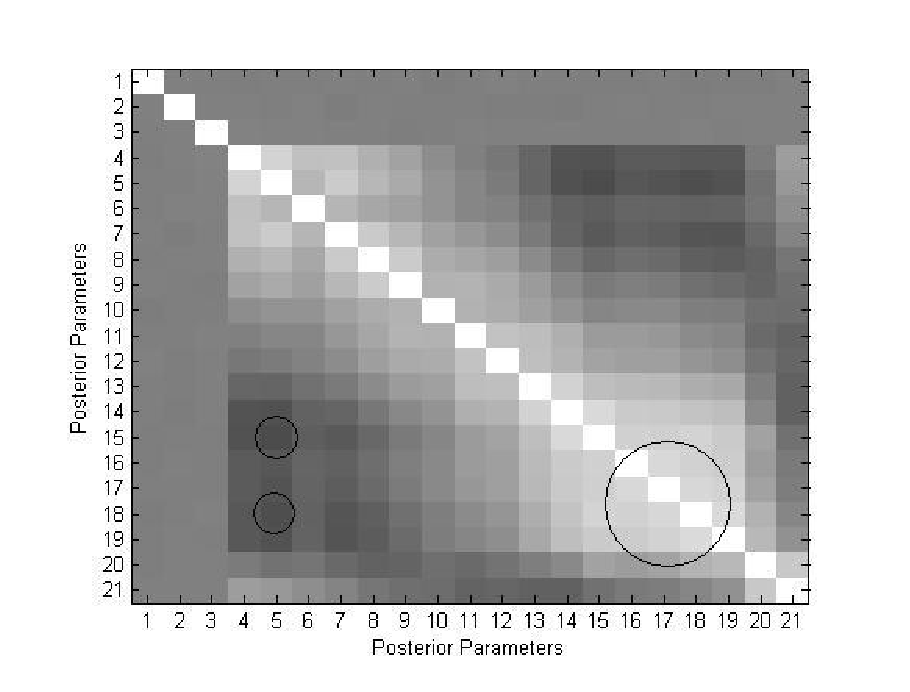
\includegraphics[width=6in]{correlation.eps}
\caption[Parameter correlation]{Parameter correlation: a grey value of 128, such as (1,21) in the lower left corner, represents no correlation. A white cell, such as (1,1) in the upper left corner, represents a correlation of 1. A black cell represents a correlation of -1. Parameters are in the following order: $T_{00},T_{01},...,T_{22},V_{00},V_{01},...V_{22},S_{0},S_{1},S_{2}.$ The big circle marks a positive correlation between parameters, and the small circles mark a negative correlation between parameters.}
\label{correlation}
\end{figure}

%---------------------------------------------------
\subsection{Prior Predictive vs. Posterior Predictive}
\label{sec:4.4}

In this section we compare the prior predictive probability distribution and the posterior predictive probability distribution. The prior predictive is generated by sampling from the prior beliefs specified in the first part of the model. The posterior predictive is generated by sampling (using MCMC) from the posterior beliefs generated from the first part of the model. If no previous human behavior data is available, then the prior predictive can still be used to show likely places to find the missing person; otherwise, the posterior predictive should be used because combining existing human behavior data enables the model to reduce uncertainty in the posterior beliefs.

Both probability distributions use a generative approach to predict how the lost person might travel from the point last seen as time progresses. The 2D probability distribution map generated is the final product of the model and can be used by Incident Commanders in WiSAR operations.

The lower row of Figure~\ref{priorvspost} shows the posterior predictive distribution created using the samples generated for all the parameters through MCMC. After 200 time steps (equivalent to 3 hours and 20 minutes), we can see that near the right side of the map, clearly much less probability mass is allocated compared with the prior predictive distribution (indicated by arrows). The center of the northern region also has lower probability compared with the prior predictive distribution, but the difference is not dramatic. Therefore, with our lost scout scenario, this posterior predictive probability distribution map suggests that we should send search and rescue workers to the regions marked by the two highest peaks first to maximize the likelihood of finding the missing scout.

%=====================================================================================================
\subsection{Bayesian \texorpdfstring{$\chi^2$}{Chi-squared} Test for Goodness-of-Fit}
\label{sec:4.5}

We used the Bayesian $\chi^2$ test for goodness-of-fit proposed by~\cite{Johnson2004Bayesian} to evaluate the  quality of posterior beliefs in the proposed model. This test is closely related to the classical $\chi^2$ goodness-of-fit statistic, but different in many aspects. The classical $\chi^2$ goodness-of-fit test computes a single $p$-value. The Bayesian version, however, computes the goodness-of-fit at each iteration of the MCMC, conditional on the current set of model parameter values sampled from the posterior distribution of all the model parameters. The posterior distribution of the resulting $p$-values converges to a $\chi^2$ distribution with $k-1$ degrees of freedom as the number of iterations approaches infinity. \cite{Johnson2004Bayesian} defined the Bayesian $\chi^2$ test for goodness-of-fit using the following equation:
\begin{align}
R^B(\vec{\tilde{\theta}}) = \sum_{k=1}^K {\left [\dfrac{(m_k(\vec{\tilde{\theta}})-n p_k)}{\sqrt{n p_k}}\right ]}^2
\end{align}
where $\vec{\tilde{\theta}}$ is a set of model parameters sampled from the posterior distribution in a single iteration, $m_k(\vec{\tilde{\theta}})$ represents the number of observations that fell into the $k$th bin, $n$ is the total number of observations, and $p_k$ is the probability assigned by the null model to this interval. Values of $p_k$ are held fixed while the bin counts $m_k(\vec{\tilde{\theta}})$ are considered as random quantities.

Because our likelihood function is a categorical distribution with 7 parameters (a discrete distribution) we used 7 bins, so $k=7$. It is worth mentioning that $p_k$ is different for each data point in our case. For each set of model parameters, we calculate the probability values (for each neighbor of the cell, into which the data point fell) for the 7 bins for each observed data point, and then sum up all the probability values for each bin across all data points. By dividing the sum for all bins, we normalize the probability value, and the result is the probability for that bin.

With $k-1=6$ degrees of freedom, we computed the $\chi^2$ distribution and then computed the quantiles (the $p$-values) for each of the 10,000 $R^B(\vec{\tilde{\theta}})$ values. The results show that only 6 out of 10,000 $p$-values are smaller than 0.05, the statistical significance value we selected. The Bayesian $\chi^2$ test of goodness-of-fit suggests that our model fits the synthetic dataset well.

%=====================================================================================================
\section{Discussions and Limitations}
\label{sec:5}

First we summarize some of the assumptions made throughout the development of the model and our rationale behind them. We assume that the state transition follows a first-order Markov process. Our argument is that the lost person is likely in a disoriented state, therefore, the assumption should not be a big problem (see section~\ref{sec:3.4.2} for more details). Another assumption is that the three terrain features are independent. Although correlation analysis shows possible dependence between terrain features, we believe it is more intuitive for domain experts to assume independence instead of specifying conditional probabilities, and we rely on data to identify the dependence relationship (see section~\ref{sec:4.3} for more details). We also assume that the Markov process is stationary with homogeneous time steps (see section~\ref{sec:3.6} and section~\ref{sec:4.4}). However, we argue that the flexibility of specifying finer time intervals and the possibility to stay in the same state can ``simulate'' a non-stationary process with various time durations, thus alleviating the restriction.

After analyzing 162 lost-person incidents near Peter Lougheed Provincial Park in Alberta, Canada, \cite{Heth1998Characteristics} come to the conclusion that there is a close correlation between a lost-person's intended destination and the angle of dispersion (calculated from the lost-person's point last seen and the point the person was eventually found). This finding suggests that it might be a good idea to incorporate the missing person's intended destination into our existing model.

One limitation of this paper is that we are using synthetic data for our evaluation. To address this, we recently collected all the GPS track logs within the US that were uploaded to the popular web GPS track log repository, everytrail.com. We were able to identify 329 GPS track logs that contained the word ``geocache'' (or ``geocaching''). Because most of the geocache ``treasures'' are hidden in the wilderness off of a designated trail, we believe that GPS track logs created by geocachers are likely to contain behavior data indicating how a human might react to different terrain features. After closer examination of these track logs, we see a clear trend that the locations of the geocache ``treasures'' play an important role in the person's behavior in the wilderness in addition to terrain features. If we want to use this kind of GPS track log data as existing human behavior data, our model has to take into consideration the intended destination.

Another trend we observed from these GPS track logs is that a majority of the geocachers first followed some trails to get closer to the ``hidden treasure''. When the trail starts to clearly lead the person further away from the geocache, or when the person decides to take a shortcut somewhere along the trail, the geocacher then abandons the trail and creates a new path.

During the summer of 2009, a student in our research lab went for a geocache hunt near Box Elder Peak in Utah. After successfully finding the ``hidden treasure'', he decided to not return the same way he came from, but to try some alternative route. Soon he found himself lost and struggled for several hours to reorient himself. Eventually he stumbled onto a hiking trail, a different one from what he took before completing the geocache mission, then he followed the trail and found his way back. Figure~\ref{BoxElderPeak} shows the GPS track log displayed in Google Earth for the period when he was off-trail and lost in the wilderness. The point we want to make here is that after running into another unknown hiking trail, he immediately decided to stay on the trail. This kind of behavior can only be predicted by models that handle trail-following, and our present model clearly lacks this capability.

We plan to extend our model to support intended destination and trail-following. Doing so would allow us to take advantage of abundant GPS track logs and incorporate such human behavior data into the posterior distribution. Once we have the newer model, we can also take advantage of the existing Bayes factor analysis methods, such as Akaike Information Criterion (AIC) proposed by~\cite{Akaike1974AIC}, Bayesian Information Criterion (BIC) presented in~\cite{Schwarz1978BIC}, and Deviance Information Criterion (DIC) described in~\cite{Spiegelhalter2002DIC}, to perform extended validation.

In the present model, for every time step, only one sample is generated from each Beta distribution. A possible improvement is to use the idea of particles. At each time step, the model would generate, for instance, 100 examples from each Beta distribution, and then compute 100 sets of categorical distributions (each has 7 discrete values representing probabilities of transitioning to 7 directions), which can then be averaged to produce a final categorical distribution with better quality and a better representation of the experts' uncertainty. Because the added computation is outside of the MCMC algorithm and the matrix multiplications, the added execution time should be minimal.

Another important question we should ask is: How well would an experienced IC trust the probability distribution map generated using the proposed model? We strongly believe that the predictive probability distribution generated using the proposed model should only be used as a base onto which domain expertise can be further projected. The objective of the model is to provide a tool that reduces the IC's workload and supports the IC's operation, but not to replace the IC's responsibilities. With abundant experience, training, and the ability to incorporate much richer information (e.g., lost person profile, weather), the IC is responsible for validating the probability distribution suggested by the model and also for coming up with the final distribution map. To really make the tool useful for ICs in WiSAR operations, two additional elements are necessary: 1) a human factors analysis (user study) of the users' trust of the algorithms and automation in the WiSAR domain, and 2) an interface component/tool that enables the IC to easily modify the probability distribution generated by the model. The ability for the IC to modify the probability distribution both at the beginning and during the search can potentially improve how (much) users trust the system and make the proposed model more acceptable to users. Future work should develop an interface tool that enables a user to modify a probability distribution map. We believe results from such research can help improve the usability and usefulness of the proposed model.

\begin{figure}
\centering
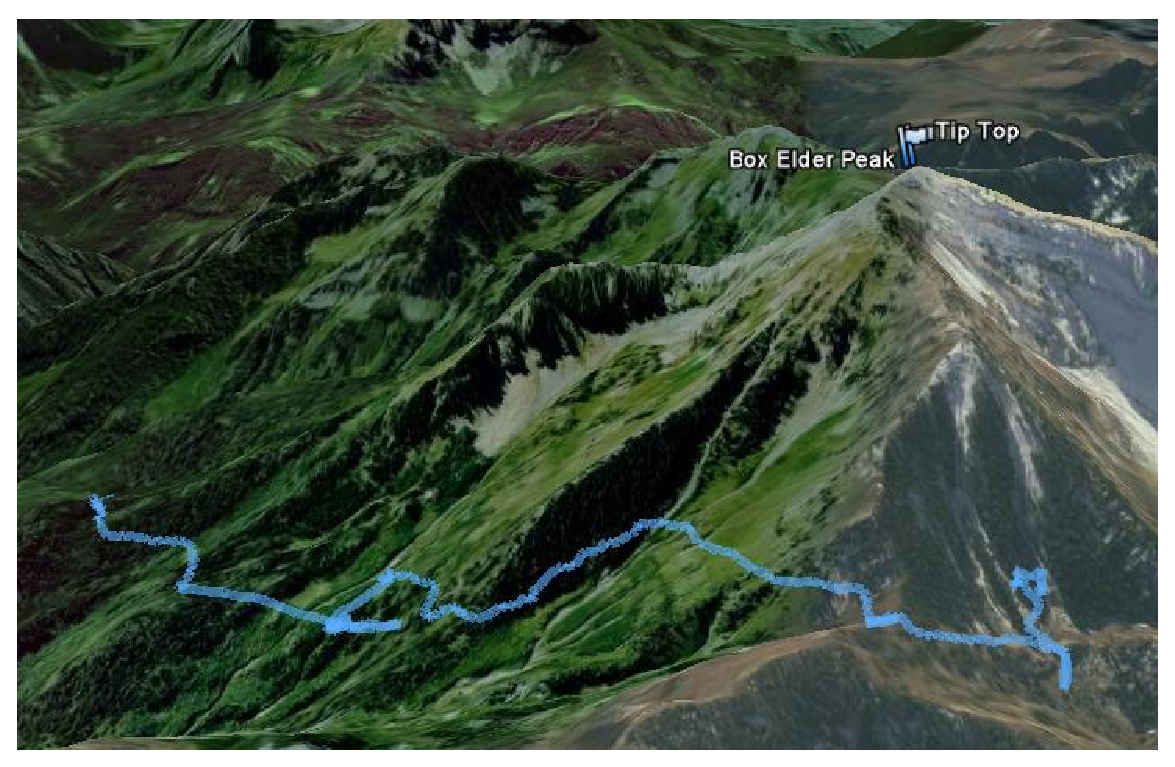
\includegraphics[width=5.5in]{BoxElderPeak.eps}
\caption[Satellite imagery of Elder Box Peak in Utah]{Satellite imagery of Elder Box Peak in Utah. The GPS track log shows the path taken by a hiker in summer 2009 when he went off the hiking trail and became lost for several hours before stumbling into another hiking trail.}
\label{BoxElderPeak}
\end{figure}



%=====================================================================================================
\section{Conclusions and Future Work}
\label{sec:6}

In WiSAR operations, the Incident Commander typically has limited resources and relies on a probability distribution map to allocate resources, to direct the search, and to coordinate rescue workers. Because as time progresses, the survivability of the missing person decreases and the effective search radius increases by approximately 3km/hour, it is critical to find the missing person quickly. That is why areas with high probabilities are searched first, and the quality of the probability distribution map can have a great impact on the search and rescue operations. We proposed a Bayesian approach to help generate such a probability distribution map by modeling lost-person behaviors based on three terrain features: topography, vegetation, and local slope. Our objectives are to ease the generation of probability distribution maps for the search and rescuers and to improve the quality of these maps.

Our proposed model uses publicly available geographic information and enables domain experts to specify uncertainty in their prior beliefs of how the missing person will transition from one terrain feature to another. Using the Bayesian model, past human behavior data in wilderness can be incorporated into the model to generate posterior beliefs. Following a first-order Markov process, the posterior beliefs can be used to build a temporal state transition matrix that allows the generation of the posterior predictive probability distribution map for any given time interval. We evaluated our model using the Bayesian $\chi^2$ test of goodness-of-fit from~\cite{Johnson2004Bayesian} because it allows the evaluation of multiple $p$-values for samples generated from the posterior parameter space. Results from the test suggest that our model fits the synthetic dataset well. The proposed Bayesian approach is promising, but we also acknowledge that the present model is limited to the proposed terrain features and could benefit from incorporating additional factors such as intended destination and trail-following.

In future experiments, we plan to let search and rescue experts specify terrain-based transitional probabilities so the prior predictive probability distribution can be generated using our model. Then we also let the experts directly specify a probability distribution on the regional map (with and without the restriction of only considering how terrain features would affect the lost-person's behavior). It would be very interesting to compare the resulting distributions and analyze the causes of any differences. However, because there is no ``ground truth'' with respect to the ``correct'' probability distribution, such comparisons will not be used as a form of validation. Instead, such information can be used to enrich prior beliefs in our model.

Future work should also explore how the generated probability distribution map can be used as a base by the search and rescue workers to reduce workload and also reduce the chance that the search and rescue workers might overlook certain areas that should have been allocated higher probabilities. It is also worth investigating what effect different spatial resolution (granularity) when sampling GPS track logs might have on the quality of the predicted probability distributions. The temporal model enables the search and rescue workers to view the dynamic changes of the probability distribution map over time. It will be beneficial to investigate further how search and rescuers can take advantage of this kind of information to improve search efficiency.

Most importantly, the proposed terrain feature-based Bayesian model is only the foundation of a larger framework. Future work should include incorporating more factors that affect lost-person behaviors into the network. Such factors include but are not limited to direction of travel, missing person profile, panicking factor, weather conditions and season of the year. The framework should allow incorporating observed data, such as a piece of clothing or candy wrapper, into the model as the search and rescue operation progresses. Our ultimate goal is to provide tools that will improve the efficiency and effectiveness of each search and rescue operation so the search and rescue workers can locate the missing persons in the minimum amount of time required, so lives can be saved.

\chapter[Paper: UAV Intelligent Path Planning for Wilderness Search and Rescue]{Paper: UAV Intelligent Path Planning for Wilderness Search and Rescue\footnote {Published in IROS 2009 (IEEE/RSJ International Conference on Intelligent Robots and Systems) conference. Authors are Lanny Lin, and Michael A. Goodrich.}}
\label{chap:IROS2009}

\begin{abstract}
In the priority search phase\footnote{Four qualitatively different types of search strategies are used in WiSAR: hasty search, constraining search, priority search, and exhaustive search. See~\cite{Goodrich2008Supporting} for more details.} of Wilderness Search and Rescue, a probability distribution map is created. Areas with higher probabilities are searched first in order to find the missing person in the shortest expected time. When using a UAV to support search, the onboard video camera should cover as much of the important areas as possible within a set time. We explore several algorithms (with and without set destination) and describe some novel techniques in solving this problem and compare their performances against typical WiSAR scenarios. This problem is NP-hard, but our algorithms yield high quality solutions that approximate the optimal solution, making efficient use of the limited UAV flying time.
\end{abstract}

%=================================================================================
\section{Introduction}

The use of mini-UAVs (Unmanned Aerial Vehicles) in Wilderness Search and Rescue (WiSAR) has gained interest for researchers and experienced advancement in recent years due to its low cost, portability, and potential field use~\cite{Goodrich2008Supporting}. The UAV onboard video camera provides visual support, enables search and rescue workers to systematically survey large areas of importance in real time~\cite{Goodrich2008Supporting,Quigley2005Towards}, and increases the workers' awareness of the environment.

For WiSAR, as time progresses, the survivability of the missing person decreases and the effective search radius increases by approximately 3km/hour~\cite{Setnicka1980Wilderness,Syrotuck2000Introduction}. Therefore, search efficiency can dramatically affect the outcome of the search and rescue. In the prioritized search phase, the incident commander creates a probability distribution map for finding the missing person based upon terrain features, profile of the missing person, weather conditions, and subjective judgment of expert searchers. Such maps can also be created systematically by utilizing geographical information available to the public via the Internet~\cite{Lin2009Bayesian,Ferguson2008GIS,Soylemez2006Utility}. UAVs have limited flying time, and in most cases, it is not long enough for the onboard video camera to cover the entire search area. For these reasons, the important question is this: given a probability distribution map, a starting point, an ending point (optional), and specified flying time, what is the best path that enables the UAV onboard video camera to ``cover'' as much of the probability distribution as possible?

Characteristics such as possibly repeated visits and probability cumulation make this a more challenging problem than standard Orienteering Problem (OP) and coverage problem. Contributions of this paper include novel path planning techniques (``global warming effect'', path crossover/mutation), additional specified-destination constraint while accumulating probability, a solid validation of the algorithms' performance, and applying algorithms to a practical, real-world application. Experimental results from this paper are conducted in simulation and not on-board a real UAV. 

%=================================================================================
\section{Problem Formulation}

We model this problem as a discretized combinatorial optimization problem with respect to probability accumulated in the 2D space for UAVs that use gimbaled cameras. Using Koopman's search metric of the instantaneous probability of detection by one glimpse~\cite{Koopman1980Search}, we assume the observer has a 100\% target detection rate. This means that as the UAV camera footprint moves along the probability distribution map, it collects (``zeros out'') all the probability along the way and accumulates the probability. A good analogy would be thinking of the UAV as a vacuum cleaner sucking up probabilities with 100\% efficiency.

In WiSAR operations, a UAV maintains an altitude of approximately 60m above ground and travels at roughly 12--13m/s~\cite{Goodrich2008Supporting}. With this height, the onboard camera footprint size comes to about 32m$\times$24m. The batteries on the UAV can keep it airborne for approximately 1--2 hours depending on weather conditions. We assume that the UAV will always maintain the same height of 60m above ground (through Height-Above-Ground automation) and travel at the constant speed of 12m/s, and use 24m$\times$24m as the effective camera footprint size. Given these parameters, a 60$\times$60 probability grid, where each probability node is 24m$\times$24m, represents an area of 2.0736km$^2$ that will take the UAV 2~hours to cover entirely. In our path planning, we restrict the direction a UAV can travel to only North, South, West and East (making only 90 degree turns), and it takes the UAV 2~seconds (1~time step) to travel from one node to its direct 4-connected neighbor. In real flights, a UAV can approximate a 90~degree turn (covering 3~nodes) in 4~seconds, so this model is close to UAV's capabilities. Also during roll or yaw, the gimbaled camera can rotate to remain aiming straight down, enabling the 90 degree turn of the camera footprint.

Using $i$ for the row number and $j$ for the column number, each probability node (cell in grid) can be written as $N_{ij}$ where $0{\leq}i,j{<}60$. The value of each $N_{ij}$ is the total volume of probability within the grid cell and thus
\begin{equation}
\sum_{i=0}^{n-1}\sum_{j=0}^{n-1}N_{ij} = 1,
\label{4totalP}
\end{equation}
where $n$=60. Let $T$ be the total number of time steps allowed for the UAV (specified flying time). Let $P$ be the set of all possible paths for the UAV on the probability grid for $T$ time steps. Each path, $p_{k} \!{\in} P$, can be represented by a sequence of probability nodes \{$N_{0},N_{1},N_{2},...,N_{T}$\} consisting of $T\!{+}1$ nodes. If the UAV is allowed to visit a node more than once, then the same node can be in a different part of the sequence.

If we use a binary variable $x_{ij}$ to represent whether $N_{ij} \!{\in} p_{k}$, $x_{ij}$ becomes a function of path $p_{k}$: 
\begin{equation}
x_{ij}(p_{k}) = 
	\left\{
	\begin{array}{cl}
		1, & N_{ij} \in p_{k} \\
		0, & \mbox{otherwise}
	\end{array}
	\right.
\label{inpath function}
\end{equation}
The number of unique nodes visited is less than or equal to the length of the path:
\begin{equation}
\sum_{i=0}^{n-1}\sum_{j=0}^{n-1}x_{i,j}(p_{k}) \leq T + 1,
\end{equation}
and the total probability accumulated, $PC_{p_{k}}$, if the UAV follows path $p_{k}$ is
\begin{equation}
PC_{p_{k}}=\sum_{i=0}^{n-1}\sum_{j=0}^{n-1}x_{ij}(p_{k})N_{ij}.
\label{pathk}
\end{equation}

The optimal path $p^* \!{\in} P$ is defined such that $\!{\forall} p_{k} \!{\in} P, PC_{p^*} \!{\geq} PC_{p_{k}}$, and our goal is to find or approximate the path $p^*$, which produces the maximum cumulative probabilities within reasonable computation time.

%=================================================================================	
\section{Related Work}

Many algorithms have been used for UAV path planning such as Voronoi Diagram with Eppstein's $k$-best paths algorithm ~\cite{Beard2005Autonomous}, A*~\cite{Quigley2005Towards}, LRTA*~\cite{Howlett2006Learning}, and Probability Roadmaps~\cite{Pettersson2006Probabilistic}. These papers focus on obstacle avoidance and sensing multiple targets. 

For path planning in searching for a target, some researchers propose to use a probabilistic model and try to maximize accumulated probability along the path. In~\cite{Hansen2007Probabilistic}, Hansen et al.\ propose three search strategies: greedy, contour, and composite search, using a probability grid. In a series of papers (e.g.~\cite{Bourgault2006Optimal,Bourgault2008Human}), Bourgault et al.\ describe a Bayesian framework for trajectory planning to maximize the chances of finding the target given restricted time using one or multiple UAVs and human systems. However, the solution uses a very simple 1-step lookahead approach which generates paths far from optimal and difficult to improve upon. Both papers do not consider the possible set destination constraint and also lack solid validation of the path efficiency.

If we disallow visiting the same node more than once, this problem falls within a variation of the Traveling Salesman Problem (TSP) called the Orienteering Problem (OP)~\cite{Ramesh1992Optimal} or the Prize-Collecting Traveling Salesman Problem (PCTSP)~\cite{Gutin2002Traveling}, both of which are NP-Hard~\cite{Sokkappa1990Cost}. Many exact solving methods for the OP have been developed~(\cite{Laporte1990Selective,Fischetti1998Solving,Ramesh1992Optimal}. These exact methods can find optimal solutions to small OP problems, but for large-scale OP problems, approximation heuristic approaches are preferred. Mittenthal and Noon~\cite{Mittenthal1992Insert} present a heuristic approach that inserts or deletes a city from the subset-tour. Tasgetiren and Smith propose a Genetic Algorithm in~\cite{Tasgetiren2000Genetic} that encodes tours using a sequence of points and uses a penalty function to help search infeasible regions. Liang and Smith present an Ant Colony Optimization approach that uses an unusual sequenced local search and a distance-based penalty function in~\cite{Liang2006Ant}. These algorithms work well with OP problems of small number of nodes (21--100 nodes) but can be slow with large number of nodes. They also don't allow repeated visits.

%=================================================================================	
\section{Path Planning Algorithms}

Because none of the path-planning algorithms we discussed above work well under our model of the problem, we developed a set of algorithms based on the following ideas: Local Hill Climbing (LHC), Convolution, and Evolutionary Algorithms (EA). We also verify the paths generated to ensure the UAV is not flying backward or going outside of the allowed search area.

\subsection{Algorithms without a Set Destination}

In situations where the operator does not have a preference for where the path should end, the following algorithms were built and evaluated.

%=============================
\subsubsection{Complete-coverage Algorithm (CC)}

The algorithm plans flight paths by following a lawnmower pattern. It first identifies the smallest $m \!{\times} n$ bounding rectangle that contains all the non-zero probability nodes. If the starting location is inside the pattern, the algorithm simply generates a path following the pattern. Otherwise, it first plans a shortest path to the edge of the bounding rectangle. When allowed flight time is large enough, this algorithm is guaranteed to collect all the probabilities.

%%=============================
%\subsubsection{Potential Fields Algorithm}
%
%The Potential Fields (PF) algorithm is based on techniques from behavior-based robotics~\cite{[06PotentialFields]Arkin}. In our implementation, each probability node emits an attractive field with a discounting factor $\gamma$, which is a function of the distance between the node and the UAV's current position. Because we are using a 4-connected approach, Manhattan distance is used, and each node emits equal attractive forces both North-South and East-West. The discounted force $f$ can be calculated as: $f = \gamma N_{ij}$, where the discounting factor $\gamma = e^{\frac{-d^{2}}{2\sigma^{2}}}$, $d$ is the distance and $\sigma$ is the standard deviation of a scaled Gaussian curve. Attractive forces in all four directions of the UAV's current position are evaluated, and the UAV follows the direction of the strongest force. In case of a tie, a random direction is selected from the tied directions. The algorithm runs the PF algorithm multiple times with $\sigma \!{=} 10, 20, ..., 120$ and then returns the best path found.

%The discount function plot is shown in Figure~\ref{PFCurves}.
%
%\begin{figure}
%\centering
%\includegraphics[width=3.5in]{PFCurves.jpg}
%\caption{Potential Field forces discount function with $\sigma=10,20,...,120$}
%\label{PFCurves}
%\end{figure}

%=============================
\subsubsection{Local Hill Climbing Algorithms (LHC)}

This is a greedy algorithm that always follows the direction with the highest value. A direct implementation of LHC does not work well with a multi-modal probability distribution map because the path generated stays with one mode until it has covered it completely before moving on to another. To address this problem, we use a global warming metaphor where the ``ocean surface'' represents all the zero-valued nodes and the ``islands'' represent the probability modes; see Fig.~\ref{GlobalWarming}. We subtract a constant $C$ from all nodes but keep all node values non-negative, where $C \!{=} \max{(N_{ij})}/l$, and $l$ defines how fine grained the search should be:
\begin{equation}
N_{ij}' \leftarrow
	\left\{
	\begin{array}{ll}
		N_{ij} - C, & N_{ij} > C \\
		0, & \mbox{otherwise}
	\end{array}
	\right.
\label{4GW}
\end{equation}
When the ocean surface rises $C$ each time, the volume of islands above water decreases, and if the ocean surface rises $l$ times, all islands will be below water. In our experiments we set $l$=40 and use the LHC algorithm to generate 40 paths: one before the ocean surface rises and one for each time the ocean surface rises (before water covers everything). We then recompute the probability accumulated for these 40 paths using the original probability grid and return the best path. This global warming technique allows the LHC algorithm to break out of one mode before completely covering that mode and move toward another. In case of a tie as to where to go next, we use two methods as the tie-breaker: LHC-GW-CONV uses a convolution kernel (with small, medium and large sizes) to determine which neighbor is more promising, and LHC-GW-PF uses Potential Fields (PF) with various discounting factors to determine where to go next.

\begin{figure}
\centering
\includegraphics[width=6in]{GlobalWarming.jpg}
\caption{Global Warming Effect}
\label{GlobalWarming}
%\vspace*{-3ex}
\end{figure}

%=============================
\subsubsection{Evolutionary Algorithms}

We developed two Evolutionary Algorithms: EA-Dir and EA-Path. Both use the probability accumulated for each path as the fitness function and employ the proportional selection method~\cite{Mitchell1997Machine}. The difference between the two algorithms lies in the path representation during crossover.

With the EA-Dir algorithm, a path is encoded as a string of directions consisting of North, East, South, and West in the crossover phase (e.g. ``NNWEE...''). Because the paths generated using single-point crossover~\cite{Mitchell1997Machine} have a very high probability of being invalid (flying out of the map), we only use double-point crossover~\cite{Mitchell1997Machine} and restrict the mid-section to a fixed 5-direction string.

With the EA-Path algorithm, a path is encoded as a sequence of node positions. If the two parent paths share only one common node, then single-point crossover is used; if they share two common nodes in the same order, then double-point crossover is used; otherwise, the two parent paths are discarded and the process starts over. For the single-point crossover method the two parent paths are crossed at the common node; see Fig.~\ref{CType1}. For double-point crossover method, the first common node and the second common node in the parent paths mark the middle sections to be swapped; see Fig.~\ref{CType2}. Both techniques could result in one longer path and one shorter path. The longer path is truncated back to the original path length and the shorter path is extended by performing crossover again and then truncating.

\begin{figure}
\begin{tabular}{cc}
\begin{minipage}[b]{0.4\linewidth}
\centering
\includegraphics[width=2.5in]{crossover1.jpg}
\caption{An example of single-point path crossover (Upper row: the parents. Lower row: the children)}
\label{CType1}
\end{minipage}
\hspace{1cm}
\begin{minipage}[b]{0.4\linewidth}
\centering
\includegraphics[width=2.5in]{crossover2.jpg}
\caption{An example of double-point path crossover (Upper row: the parents. Lower row: the children)}
\label{CType2}
\end{minipage}
\end{tabular}
%\vspace*{-4ex}
\end{figure}

Two types of mutation methods~\cite{Mitchell1997Machine} are used for flight path evolution; see Fig.~\ref{Mutation}. They follow a greedy approach with the hope that small positive changes to the path will lead to larger positive changes to the path. First we randomly select a node in the flight path and see if the next two nodes along the path would form an L shape with this node or a straight line (these are the only two possibilities). In the first case, method~1 (``flip'') is used and the algorithm replaces the middle node with the node that mirrors the middle node if we connect the first node and the third node with a line. This is like flipping a section of the path. In the second case, method~2 (``pull'') is used and the algorithm inserts two nodes into the path on one side of the line next to the first and the second nodes. This effectively extends the path by two nodes, so we simply truncate the last two nodes from the path. This is like pulling a string from the middle when the beginning end of the string is fixed. Which side to select for insertion depends on whether the new path is a valid path. If both sides allow valid paths, then the algorithm prefers inserting nodes that are not already in the path. Random selection is the last tie-breaker. If all four nodes on either side of the line are already included in the path, then a new mutation point is randomly selected and the same procedure repeats.

%\begin{figure}
%\begin{tabular}{cc}
%	\begin{minipage}{0.25\textwidth}
%	\flushright 
%	\includegraphics[width=1in]{m1_1.jpg}
%	\end{minipage}
%	\begin{minipage}{0.25\textwidth}
%	\flushleft
%	\includegraphics[width=1in]{m1_2.jpg}
%	\end{minipage}\\
%\end{tabular}
%\begin{tabular}{cc}
%	\begin{minipage}{0.25\textwidth}
%	\flushright 	
%	\includegraphics[width=1in]{m2_1.jpg}
%	\end{minipage}
%	\begin{minipage}{0.25\textwidth}
%	\flushleft
%	\includegraphics[width=1in]{m2_2.jpg}
%	\end{minipage}\\
%\end{tabular}
%\caption{Before and after mutation. (Upper: method 1. Lower: method 2)}
%\label{Mutation}
%\end{figure}

\begin{figure}
\begin{tabular}{cc}
\begin{minipage}[b]{0.40\linewidth}
\centering
\includegraphics[width=2.5in]{mutation.jpg}
\caption{Examples of mutations in EA-DIR and EA-Path algorithms. (Upper row: method 1. Lower row: method 2)}
\label{Mutation}
\end{minipage}
\hspace{1cm}
\begin{minipage}[b]{0.40\linewidth}
\centering
\includegraphics[width=2.5in]{mutationE.jpg}
\caption{Examples of mutations in EA-Path\_E algorithm. ~\\ (Upper row: method 2. Lower row: method 3)}
\label{MutationE}
\end{minipage}
\end{tabular}
%\vspace*{-4ex}
\end{figure}

We use an initial population of 100 paths including various paths generated using other algorithms and 95 randomly generated paths. LHC-GW-PF is not used because it is too slow. Other parameters include replacement rate at 30\% and mutation rate at 50\%. The best three paths are always kept in each iteration. The algorithm runs for at least 500 iterations and stops if either the best path does not improve after 200 iterations or if the algorithm has completed 1000 iterations.


%=================================================================================	
\subsection{Algorithms with a Set Destination}

In WiSAR, an operator might prefer the path to end at a specific destination node to support UAV retrieval, persistent visualization of a specific region at a specific time, or planning multiple path segments that make up a longer path. The following algorithms are modified versions from the previous section to handle the additional requirement. We simply add ``\_E'' to the algorithm names to distinguish them.

%=============================
\subsubsection{Complete-coverage Algorithm (CC\_E)}

This algorithm is identical to the CC algorithm up to the time when the remaining flight time is just enough to fly the UAV to the end node, then it flies toward the end node using the LHC-GW-CONV\_E algorithm (discussed shortly).

%%=============================
%\subsubsection{Potential Fields Algorithm}
%
%The PF\_E algorithm is similar to the PF algorithm except it is more constrained. During path generation, when choosing which node to go next, if going to the node makes it impossible to get to the end node within the remaining flight time, the node will not be selected. This simple constraint causes the algorithm to generate a path that allows the UAV to arrive at the end node at exactly the end of the specified flight time.

%=============================
\subsubsection{Local Hill Climbing Algorithms}

The LHC-GW-CONV\_E and LHC-GW-PF\_E algorithms have an additional constraint where nodes that prevent the path from reaching the end node within the remaining time will not be selected.

%=============================
\subsubsection{Evolutionary Algorithm}

The direction representation of a path does not work with a set destination, so the EA-Path\_E algorithm also uses a sequence of node positions to encode the path. Here we increased mutation rate to 90\% to force more exploration of the state space. The initial population of 100 paths includes various paths generated using other algorithms as seeds (both from start node to end node and reversed) and 90 randomly generated paths.

The EA-Path\_E algorithm uses both single-point and double-point crossover. The difference is that when the child path is too long, the algorithm truncates the path to the original path length, then backtracks the path until the distance between the end of the child path and the desired end node matches the remaining time. The LHC-GW-CONV\_E algorithm is then used to complete the path with the desired end node. If the child path is too short, the LHC-GW-CONV\_E algorithm is used to complete the path.

The EA-Path\_E algorithm uses three types of mutation methods. First, we randomly select a node in the path and see if the next two nodes along the path would form an L shape with this node or a straight line. In the first case, method~1 (``flip'') is used (identical to the one used in the EA-Path algorithm); see Fig.~\ref{Mutation}. If the nodes form a straight line, then method~2 (``pull'') or 3 (``shake'') is selected with equal probabilities; see Fig.~\ref{MutationE}.

Mutation method~2 (``pull'') is a modified version from the EA-Path algorithm. This method does not truncate two nodes at the end of the path; instead, it deletes two nodes in the middle of the path. This is like pulling a string from the middle when both ends of the string are fixed.

Mutation method~3 (``shake'') works by first marking a small mid-section in the path (to keep it short, we set it to 6 nodes). We first randomly select a node in the path, then traverse the path and find the fifth node down the path. If the path between these two nodes is not a straight line, the method replaces the mid-section with random flying while maintaining the same length for the mid-section. This is similar to shaking a chain where the beginning and ending points remain fixed but the middle section shifts.

%\begin{figure}
%\begin{tabular}{cc}
%	\begin{minipage}{0.25\textwidth}
%	\flushright 
%	\includegraphics[width=1in]{mE2_1.jpg}
%	\end{minipage}
%	\begin{minipage}{0.25\textwidth}
%	\flushleft
%	\includegraphics[width=1in]{mE2_2.jpg}
%	\end{minipage}\\
%\end{tabular}
%\begin{tabular}{cc}
%	\begin{minipage}{0.25\textwidth}
%	\flushright 	
%	\includegraphics[width=1in]{mE3_1.jpg}
%	\end{minipage}
%	\begin{minipage}{0.25\textwidth}
%	\flushleft
%	\includegraphics[width=1in]{mE3_2.jpg}
%	\end{minipage}\\
%\end{tabular}
%\caption{Before and after mutation. (Upper: method 2. Lower: method 3)}
%\label{MutationE}
%\end{figure}


%=============================
\section{Experimental Results and Analysis}

%=============================
\subsection{Performance Metrics}

We use $\mathit{Efficiency}$, $\mathit{Efficiency_{LB}}$ and Running Time as metrics to measure the performance of the algorithms, where $\mathit{Efficiency}$ is calculated if we know what's the best possible and $\mathit{Efficiency_{LB}}$ is used as an estimation when we have no way of calculating the best possible. Sorting all the probability nodes by their values in descending order would generate a list \{$N_1, N_2, N_3, ..., N_{3600}$\}. For the best possible path $p^*$, the probability accumulated $PC_{p^*}$ is constrained by a theoretical upper bound $B$:
\begin{equation}
PC_{p^*} \leq \sum_{n=1}^{T+1-d}N_n = B,
\label{topN}
\end{equation}
where $d$ is the distance from the start node to the closest non-zero valued node. Then for any path $p_k$, we define $\mathit{Efficiency}$ and $\mathit{Efficiency_{LB}}$ as the following:
\begin{equation}
\mathit{Efficiency} = \frac{PC_{p_k}}{PC_{p^*}}
\label{4Efficiency}
\end{equation}
\begin{equation}
\mathit{Efficiency_{LB}} = \frac{PC_{p_k}}{B}
\label{4EfficiencyLB}
\end{equation}
$PC_{p_k}$ can be calculated using~(\ref{pathk}). $\mathit{Efficiency}$ can be calculated when $PC_{p^*}$ is known and $\mathit{Efficiency_{LB}}$ can be calculated anytime. Clearly, $\mathit{Efficiency_{LB}} \leq \mathit{Efficiency}$.

For example, a path with 95\% $\mathit{Efficiency}$ means the amount of probability accumulated following this path is 95\% of the maximum possible. A path with 85\% $\mathit{Efficiency_{LB}}$ means the probability accumulated is 85\% of the maximum amount possible if the UAV can teleport from node to node, and the true $\mathit{Efficiency}$ could be much higher.

All experiments are run on a Dual-core AMD 3800+ PC with 1GB of memory. For each algorithm, running time is recorded so we can compare algorithm speed.


%=============================
\subsection{Typical WiSAR Scenarios}

In our experiments, we focus on probability distribution maps of three abstract but representative WiSAR scenarios: unimodal, bimodal, and bimodal with overlap. The top row of Fig.~\ref{maps} shows the 2D representations where each pixel is a probability node; the lighter the pixel, the higher the probability value. The middle row shows three simplified versions of the distributions, which can be used to manually identify the best path possible for each map and compute $PC_{p^*}$. Then we can measure the true $\mathit{Efficiency}$ of paths generated. The blue arrows on the maps mark the starting node (possible location for a WiSAR command center) and the red dots mark the ending node (intentionally selected at a different region from the starting nodes). The bottom row shows the best paths generated for the real maps at $T$=900.

\begin{figure}
\centering
\includegraphics[width=4.75in]{maps900.jpg}
\caption{Top row: 2D representations of unimodal, bimodal, and bimodal with overlap probability distribution maps. Middle row: Simplified versions of the three types of maps. Bottom row: Best paths found for each map.}
\label{maps}
%\vspace*{-4ex}
\end{figure}


%=============================
\subsection{Experimental Results and Analysis}

For each distribution type (real and simplified maps) we ran each algorithm (with or without set destination) using $T$=120, 300, and 900 (4, 10, and 30 minutes). Because of random factors, we ran each experiment 10 times and calculated mean and standard deviation of the results. Due to space limitation, only a subset of the experimental results are presented (e.g. Table~\ref{EBimodalSimplified}, \ref{TBimodalSimplified} and Figure~\ref{graphBimodal}--\ref{graphRealSimple}).

For all the experiments we performed, algorithm running time exhibited the same trend: from the fastest to the slowest we have LHC-GW-CONV(\_E), EA(\_E) and LHC-GW-PF(\_E). For example, with the simplified unimodal map, the LHC-GW-PF algorithm ran for 9.419, 41.952 and 164.383 seconds for $T$=120, 300 and 900 respectively. Because the EA(\_E) algorithms use the path generated from other algorithms as seeds in the initial population, they are generally slower. However, most of the running time is spent generating the initial population and the evolutionary part of these algorithms only takes a fraction of a second. LHC-GW-PF(\_E) algorithms are always the slowest, and that is why we do not include them as seeds in the EA algorithms. For the group of algorithms with set destination, we perform path planning both from the starting node to the ending node and also from the ending node to the starting node (then reverse the path), and then select the better one; we include both runs when we record the algorithm running time. Therefore, the ``\_E'' algorithms always take more time to complete compared to the version before modification.

For the simplified unimodal map, the LHC-GW-CONV(\_E) algorithms are the clear winners in each respective group if we consider both the $\mathit{Efficiency}$ and the running time. For the group of algorithms without set destination, all algorithms gave above $99.5\%$ $\mathit{Efficiency}$. The LHC-GW-CONV algorithm is always the fastest  (e.g. 6.483 seconds for $T$=900) and achieved 100\% $\mathit{Efficiency}$ in all cases. The EA-Dir and EA-Path algorithms also achieved 100\% $\mathit{Efficiency}$, but at a much slower speed (e.g. 62.236 seconds for $T$=900 with EA-Path). For the group of algorithms with set destination, the LHC-GW-CONV\_E algorithm is also the fastest  (e.g. 14.173 seconds for $T$=900) and achieved 99.955\% or higher $\mathit{Efficiency}$ in all cases. Although the EA-Path\_E algorithm achieved slightly better $\mathit{Efficiency}$ (less than 0.1\% improvements), it did so at the cost of more running time (e.g. 78.334 seconds for $T$=900).

For the simplified bimodal map, the LHC-GW-CONV(\_E) algorithms did not always perform well because it doesn't handle the space between the two modes very well, especially for very short flight time. Fig.~\ref{graphBimodal} shows the $\mathit{Efficiency}$ comparison of the group of algorithms without set destination. The LHC-GW-PF(\_E) algorithms still achieved 96\% and above $\mathit{Efficiencies}$, but they are also the slowest. The EA(\_E) algorithms are more attractive in this case because they achieved the best $\mathit{Efficiencies}$ (98.095\%+ for EA and 97.857\%+ for EA\_E) very quickly.

\begin{table}
%\small
	\centering
		\begin{tabular}
			{|l|c|c|c|c|c|c|}
			\hline
			(\%) & \multicolumn{3}{|c|}{Simplified ({\it{Efficiency}})} & \multicolumn{3}{|c|}{Real ({\it{Efficiency$_\textrm{LB}$}})} \\
			\hline
			$T$ & 120 & 300 & 900	& 120 & 300 & 900 \\
			\hline
			LHC-GW-CONV & 88.89 & 96.80 & 98.35 & 81.64 & 93.97 & 97.75 \\
			\hline			
			LHC-GW-PF	& 96.63 & 96.70 & 96.07 & 90.28 & 92.43 & 96.67 \\ 
			\hline
			EA-Dir & 98.59 & 97.31 & 98.80 & 90.62 & 94.96 & 97.96 \\
			\hline
			EA-Path & 98.66 & 98.09 & 99.07 & 91.18 & 95.71 & 98.02 \\
			\hline
		\end{tabular}
\caption{Algorithm efficiency comparison for bimodal distribution}
\label{EBimodalSimplified}
%\vspace*{-5ex}
\end{table}

\begin{table}
	\centering
		\begin{tabular}
			{|l|c|c|c|c|c|c|}
			\hline
			(seconds) & \multicolumn{3}{|c|}{Simplified} & \multicolumn{3}{|c|}{Real} \\
			\hline
			$T$ & 120 & 300 & 900	& 120 & 300 & 900 \\
			\hline
			LHC-GW-CONV & 0.90 & 2.26 & 7.35 & 0.52 & 1.16 & 5.66 \\
			\hline
			LHC-GW-PF	& 9.44 & 29.11 & 131.35 & 2.61 & 8.64 & 92.38 \\
			\hline
			EA-Dir & 9.36 & 15.56 & 41.71 & 10.97 & 16.69 & 35.11 \\
			\hline
			EA-Path & 10.63 & 22.89 & 66.31 & 12.61 & 21.20 & 53.73 \\
			\hline
		\end{tabular}
\caption{Algorithm speed comparison for bimodal distribution}
\label{TBimodalSimplified}
%\vspace*{-7ex}
\end{table}

\begin{figure}
%\vspace*{-2ex}
\centering
\includegraphics[width=6in]{graphBimodal.jpg}
\caption{$\mathit{Efficiency}$ comparison for group of algorithms without set destination for simplified bimodal map}
\label{graphBimodal}
%\vspace*{-2ex}
\end{figure}

For the simplified bimodal with overlap map, the EA(\_E) algorithms achieved the best $\mathit{Efficiencies}$ (98.302\%+ for EA and 98.653\%+ for EA\_E), but the LHC-GW-CONV(\_E) algorithms were able to achieve equivalent or slightly lower Efficiencies (97.391\%+ for LHC-GW-CONV and 98.429\%+ for LHC-GW-CONV\_E) with much less time (8.283 seconds and 16.296 seconds for $T$=900 respectively). Fig.~\ref{graphEBimodalOverlap} shows the $\mathit{Efficiency}$ comparison of the group of algorithms with set destination.

\begin{figure}
\centering
\includegraphics[width=6in]{graphEBimodalOverlap.jpg}
\caption{$\mathit{Efficiency}$ comparison for group of algorithms with set destination for simplified bimodal with overlap map}
\label{graphEBimodalOverlap}
%\vspace*{-4ex}
\end{figure}

For each of the three real distribution maps (unimodal, bimodal, and bimodal with overlap), since $PC_{p^*}$ is unknown, we can only calculate $\mathit{Efficiency_{LB}}$. We observed that the $\mathit{Efficiency_{LB}}$ for each real map is very close to the $\mathit{Efficiency_{LB}}$ for each of the counterpart simplified maps, and we hypothesize that the $\mathit{Efficiency}$ for each real map should also be close to the $\mathit{Efficiency}$ for each of the counterpart simplified maps. Fig.~\ref{graphRealSimple} shows an example of the EA-Path algorithm performance for the real and simplified bimodal with overlap map. The columns in the front row are $\mathit{Efficiency_{LB}}$ values and the columns in the back row are $\mathit{Efficiency}$ values. Based on this graph, we estimate that the $\mathit{Efficiency}$ values for the real map here are above 97\% for all $T$ values.

\begin{figure}
%\vspace*{-3ex}
\centering
\includegraphics[width=6in]{graphRealSimple.jpg}
\caption{EA-Path performance for the real and simplified bimodal with overlap map}
\label{graphRealSimple}
\end{figure}

To further evaluate our algorithms, we tested our algorithms on a more complex multimodal distribution map generated by mixing multiple Gaussian distributions with various standard deviations; see Fig.~\ref{ComplexMap}. The LHC-GW-CONV algorithm achieved 97.206\% $\mathit{Efficiency_{LB}}$ in 5.516 seconds and the EA-Path algorithm achieved 97.609\% $\mathit{Efficiency_{LB}}$ in 63.984 seconds. Note here that the $\mathit{Efficiency}$ percentiles can only be better.

\begin{figure}
\centering
\includegraphics[width=6in]{ComplexMap3.jpg}
\caption{More complex multimodal probability distribution map}
\label{ComplexMap}
%\vspace*{-3ex}
\end{figure}

In every experiment, the EA(\_E) algorithms always achieved the best $\mathit{Efficiency}$ and $\mathit{Efficiency_{LB}}$. Therefore, if the operator has some time for computation, they seem to be attractive candidates. If the operator needs a path generated quickly, the LHC-GW-CONV(\_E) algorithms can be used. Although the LHC-GW-PF(\_E) algorithms do not work as well with these three distribution maps, initial tests on other distribution types such as sparse map and small-multimodal map suggest that they could perform better than other algorithms.


%=================================================================================	
\section{Conclusion and Future Work}

We model the UAV path planning problem in WiSAR as a discretized combinatorial optimization problem and design two groups of algorithms for path planning with or without a set destination using algorithms based on Local Hill Climbing, and Evolutionary Algorithms using novel techniques such as ``global warming effect'' and path crossover/mutation. We evaluate the performances of these algorithms on six (3 simplified, 3 ``real'') representations of typical WiSAR probability distribution maps, unimodal, bimodal, and bimodal with overlap, with various flight times and use the simplified maps to validate true efficiencies in real maps. Experimental results show that our algorithms can generate good paths with high $\mathit{Efficiency}$ or estimated $\mathit{Efficiency}$ that approximate the optimal solution within reasonable computation time. Specifically, the LHC-GW-CONV(\_E) algorithms should be used for unimodal maps, and if a few minutes computation time is available, because the EA(\_E) algorithms always keep the best path found from seed algorithms, they can always find a path with the highest $\mathit{Efficiency}$ compared with other algorithms experimented.

Experimenting with more types of distribution maps, designing a more advanced global warming search model, allowing 8-connected path planning, and dealing with dynamic distribution maps that change over time are all natural extensions for future work. Specifically, the set of algorithms with set destinations enables us to further investigate how the path planning task can be segmented so human operators can plan more strategically while the algorithms plan tactically, and what interface can make this an intuitive, smooth, and effective task for the UAV operator in WiSAR operations.

\chapter[Paper: Hierarchical Heuristic Search Using A Gaussian Mixture Model for UAV Coverage Planning]{Paper: Hierarchical Heuristic Search Using A Gaussian Mixture Model for UAV Coverage Planning\footnote {Submitted to and accepted by SMC-B (IEEE Transactions On Systems, Man And Cybernetics Part B, Cybernetics) journal. Authors are Lanny Lin, Michael A. Goodrich and Spencer Clark}}
\label{chap:SMCB2014}

\begin{abstract}
During UAV search missions, efficient use of UAV flight time requires flight paths that maximize the probability of finding the desired subject. The probability of detecting the desired subject based on UAV sensor information can vary in different search areas due to environment elements like varying vegetation density or lighting conditions, making it likely that the UAV will only be partially able to detect the subject. This adds another dimension of complexity to the already difficult (NP-hard) problem of finding an optimal search path. We present a new class of algorithms that account for partial detection in the form of a task-difficulty map and produce paths that approximate the payoff of optimal solutions. The algorithms use the \textit{Mode Goodness Ratio} heuristic, which uses a Gaussian Mixture Model to prioritize search subregions. The algorithms search for effective paths through the parameter space at different levels of resolution. We compare the performance of the new algorithms against two published algorithms (Bourgault's algorithm and LHC-GW-CONV algorithm) in simulated searches with three real search and rescue scenarios, and show that the new algorithms outperform existing algorithms significantly and can yield efficient paths that yield payoffs near the optimal.  
\end{abstract}


%\begin{IEEEkeywords}
%Unmanned aerial vehicles, path planning, navigation, hierarchical systems, heuristic algorithms
%\end{IEEEkeywords}
%
%\IEEEpeerreviewmaketitle

%=================================================================================
\section{Introduction}
\label{sec:Introduction}

%\IEEEPARstart

Mini-UAVs (Unmanned Aerial Vehicles) are becoming useful tools in many reconnaissance, remote-sensing, surveillance, and search operations thanks to advances in UAV technologies. They can help firefighters map forest fires, help news crews provide coverage, help police monitor crowds, and help wilderness search and rescue workers locate a missing person. In these applications, the UAV uses its on-board cameras to provide useful visual information in support of the specific operation.

This paper focuses on using mini-UAVs to support Wilderness Search and Rescue (WiSAR). The aerial view from a UAV enables WiSAR workers to survey large areas of importance in real time~\cite{Goodrich2008Supporting}. Search efficiency is very important in WiSAR because, as time progresses, the survivability of the missing person decreases and the effective search radius increases by approximately 3km/hour~\cite{Syrotuck2000Introduction}. Therefore, a good flight path should rapidly maximize the probability of finding the missing person to make efficient use of the limited flying time.

Each UAV path accumulates information over time as the UAV's sensors scan the ground. As illustrated in Fig.\ref{TwoApproaches}, various paths do so in different ways depending on how information is distributed in the environment. The goal is to maximize the total probability of detection. There are two quality metrics for the probability-maximizing path planning problem~\cite{Koopman1957Theory, Stone1975Theory, Washburn1981Search}. First, find the path that maximizes the Cumulated Detection Probability (CDP) after a specific flight time (blue vertical dotted line). Out of the three example paths in Fig.
\ref{TwoApproaches} path 3 becomes the winner. Second, find the path that achieves a desired CDP in the shortest amount of time (red horizontal dotted line). Path 1 would become the winner out of the three, instead. We model the problem following the first approach.
\begin{figure}
\centering
\includegraphics[width=5in]{Approaches.jpg}
\caption[Two approaches to the probability-maximizing path planning problem]{Two approaches to the probability-maximizing path planning problem. With three paths generated by various algorithms, the first approach prefers the path maximizing the Cumulated Detection Probability (CDP) given a specific flight time (Path 3 is the winner) and the second approach prefers the path achieving a specified CDP in the shortest amount of time (Path 1 is the winner)}. 
\label{TwoApproaches}
%\vspace*{-3ex}
\end{figure}

When using a UAV's on-board camera to assist WiSAR operations, factors such as dense vegetation, lighting conditions, shadows, or distance between the camera and the ground can lower the quality of the UAV aerial view and decrease the probability of detection~\cite{Morse2010UAV}. This can be attributed to both sensor and human limitations (such as limited attention span and cognitive workload). We propose to represent \textit{partial detection} in the form of a task-difficulty map, where a more difficult subregion on the map has lower probability of detection. Using a task-difficulty map enables us to integrate geo-referenced and spatial-related sensor constraints into the problem formulation, which supplements traditional sensor modeling methods (e.g.,~\cite{Bourgault2006Optimal}) and potentially improves search performance in real world search scenarios. Because detection difficulties vary in different search subregions, flying patterns such as lawnmower and Zamboni don't guarantee optimal coverage. Integrating the task-difficulty map into path planning adds another dimension of complexity to the already difficult problem and causes the performance of existing greedy-type algorithms (Bourgault's Algorithm~\cite{Bourgault2006Optimal} and LHC-GW-CONV~\cite{Lin2009UAV}) to suffer.

We model the path planning problem as a discrete combinatorial optimization problem, and propose a new heuristic, the \textit{Mode Goodness Ratio}. This heuristic uses a Gaussian Mixture Model to identify and prioritize search subregions. We then present two new algorithms (\textit{Top2} and \textit{TopN}) that utilize the heuristic in hierarchical path planning by forcing the UAV to visit high priority subregions. The hierarchical structure enables the algorithms (a) to cluster probability volumes and (b) to prioritize search subregions at different levels of resolution. It also makes it easy to parallelize the two new algorithms and improve computation speed. We compare the performance of the new algorithms against two published algorithms (Bourgault's Algorithm~\cite{Bourgault2006Optimal} and LHC-GW-CONV algorithm~\cite{Lin2009UAV}) in simulated searches based on three real search and rescue scenarios. Results show that the new algorithms outperform existing algorithms significantly and can yield efficient paths that approximate the payoff of the optimal path.

The contributions of the paper are (a) the introduction of Gaussian Mixture Model (GMM) to compute the Mode Goodness Ratio heuristic, which can be used to prioritize search subregions in a hierarchical planner, (b) two new path planning algorithms that utilize the Mode Goodness Ratio heuristic to improve path-planning performance, and (c) the use of a spatial representation (task-difficulty map) in modeling sensor detection probability with terrain and vegetation information and incorporating that into UAV path planning.

Section~\ref{sec:ProblemFormulation} defines the problem and the metrics used to evaluate algorithm performance. Section~\ref{sec:RelatedWork} discusses related literature. Section~\ref{sec:PathPlanningAlgorithms} first reviews two existing algorithms and then demonstrates the weakness of these algorithms with a synthetic scenario. This section then presents the \textit{Mode Goodness Ratio} heuristic and the two new algorithms (\textit{Top2} and \textit{TopN}). Section~\ref{sec:ExperimentResultsAndAnalysis} compares algorithm performance with three real search and rescue scenarios. Section~\ref{sec:LimitationsAndDiscussion} discusses the limitations of the approach, and Section~\ref{sec:Summary} presents the summary.


%=================================================================================
\section{Problem Formulation}
\label{sec:ProblemFormulation}

%=============================
\subsection{Problem Framework}

Typical UAVs (fixed-wing or rotorcraft) are highly mobile and variable, but we will assume a set of useful constraints on their capabilities: they have a gimbaled camera, can maintain a constant height above ground and can travel at constant speed. A gimbaled camera enables the camera to aim straight down even when the UAV is performing roll or yaw maneuvers. We assume that the UAV's speed is much higher than the speed of the missing person and treat the missing person as stationary. At every UAV flight time step, we treat the camera footprint of the search area as a glimpse. This way we can discretize the search area, and model the UAV path planning problem as a discrete combinatorial optimization problem with respect to probability accumulated and define it following the framework described in~\cite{Trummel1986Technical}.

The search space is represented as a finite, connected graph $G = (V, E)$. $V$ denotes the set $\{v_1, ..., v_n\}$ of vertices of $G$, and $E$ denotes the set of edges. Each edge in $E$ can be viewed as an unordered pair of vertices $\{v_i, v_j\}$. The missing person is located at one of the vertices of $G$. A given probability distribution map for the missing person is discretized to match graph $G$, with $p_i$ being the probability that the missing person is located at vertex $v_i$. It is obvious that
\begin{equation}
\sum_{i=1}^{n}p_i = 1.
\label{totalP}
\end{equation}

The UAV search is conducted in discrete time. During each time step, the UAV camera footprint can cover one vertex. For a desired flight with $T$ time steps, let $S$ denote the set $\{0,1,2,...,T\}$. The UAV's motion is constrained by the structure of the graph $G$. Let $\Psi$ be the set of functions $\psi:S \mapsto V$ with the property that for any two consecutive integers $t$ and $t+1$ in $S$, either $\psi(t)=\psi(t+1)$ or $\{\psi(t),\psi(t+1)\}\in E$. Here $\Psi$ represents all possible paths, and under path $\psi$, vertex $\psi(t)$ is searched during step $t$. The conditions on the set $\Psi$ guarantee that at each time step the UAV camera footprint will either remain at the current vertex (only possible for a rotorcraft) or move to a neighboring vertex.

Even when the UAV camera footprint covers the vertex occupied by the missing person, it is not certain that a detection will occur. The probability of detection is described by a glimpse probability function $g$, which is defined by a given task-difficulty map. The task-difficulty map is a spatial representation of sensor detection probability and defines areas where it is difficult to detect the missing person (with lower probability of detection), with $d_i$ being the task-difficulty level at vertex $v_i$. Let $d_{max}$ be the maximum task-difficulty level in the given map. If at time step $t$ the UAV camera footprint covers vertex $v$, then let $g(v,t)$ be the probability that a detection will occur, given that the missing person is at vertex $v$. We model this as
\begin{equation}
g(v_i,t) = 1 - \frac{d_i}{d_{max}+1}.
\label{g}
\end{equation}
so that more difficult tasks (higher $d_i$ values) have lower glimpse detection values, $g$.

Let $P_T(\psi)$ represent the Cumulative Detection Probability (CDP) for path $\psi \in \Psi$ with $T$ time steps. For each (cell, time) pair $(i,t)$ with $1 \leq i \leq n$ and $0 \leq t \leq T$, we define the probability of failure $f(i,t,\psi)$ by 
\begin{equation}
f(i,t,\psi) = 
	\left\{
	\begin{array}{ll}
		1-g(v_i,t) & \mbox{if~} \psi(t)=v_i \\
		1 & \mbox{otherwise.}
	\end{array}
	\right.
\label{OneVertex}
\end{equation}
Let $D_j$ represent a detection on the $j$th observation so $\overline{D}_j$ is a detection failure. Then the probability of failing to detect the the missing person after $N$ observations of vertex $v_i$ given the missing person is at vertex $v_i$ is the joint probability $P(\overline{D}_1, \overline{D}_2, ..., \overline{D}_N|v_i)$. Assuming each observation is conditionally independent of each other (typical in the WiSAR literature), we can rewrite the joint probability as
\begin{equation}
P(\overline{D}_{1:N}|v_i) = \prod_{j=1}^{N}P(\overline{D}_j|v_i),
\label{NoDetection}
\end{equation}
and the probability of detecting the missing person after $N$ observations is
\begin{equation}
P(D_{1:N}|v_i) = 1 -  P(\overline{D}_{1:N}|v_i),
\label{Detection}
\end{equation}
which is equivalent to
\begin{equation}
P(D_{1:N}|v_i) = 1 -  \prod_{t=0}^{T}f(i,t,\psi),
\label{Detection2}
\end{equation}
where $N$ is how many times $v_i$ shows in path $\psi$. Then $P_T(\psi)$ can be computed by
\begin{equation}
P_T(\psi) = \sum_{i=1}^{n}p_i\Big(1 - \prod_{t=0}^{T}f(i,t,\psi)\Big),
\label{CDP}
\end{equation}
where $p_i$ is the probability that the missing person is located at vertex $v_i$. Define $\exists\psi^* \!{\in} \Psi$ such that for any alternate path $\psi' \!{\in} \Psi, P_T(\psi^*) \!{\geq} P_T(\psi')$. Our goal is to find the optimal path $\psi^*$ that produces the maximum CDP (path 3 in~Fig.\ref{TwoApproaches} at $T=600$ if there are only three possible paths) or find an efficient path $\psi'$ that produces payoff approximating the payoff of the optimal path within reasonable computation time.

When the path needs to end at an operator-specified vertex (for easy UAV retrieval or to join with other path segments), we simply add the constraint to the problem formulation (only add edges to a path that does not violate the constraint so the UAV has enough time to reach the end point). Also for fixed-wing UAVs, additional motion constraints (such as not allowing the UAV to fly backward) are also introduced as velocity constraints affecting edges $\{\psi(t), \psi(t_1)\}$, effectively creating a directed graph. Both proposed path planning algorithms satisfy these constraints.

%=============================
\subsection{Performance Metrics}

%Let $\mathit{Efficiency_{LB}}$ (Efficiency Lower Bound) and algorithm Run Time producing path $\psi'$ denote metrics to measure the performance of the algorithms. 
We will use two measures of algorithm performance: the quality of the path and the run-time of the algorithm. Run-time is self-explanatory, but we need a measure of path quality. Ideally the efficiency of an algorithm should be computed with the following equation:
\begin{equation}
\mathit{Efficiency}(\psi') = \frac{P_T(\psi')}{P_T(\psi^*)},
\label{Efficiency}
\end{equation}
where $\psi^*$ is the optimal path. However, because we do not know what $\psi^*$ is, we bound the efficiency. Let $\psi_{teleport}$ be defined as the path constructed as follows: (a) deduct the time needed to move from the start vertex to the nearest vertex with non-zero $p_i$ (plus time for doing the same with the end vertex if specified), and (b) at each step the UAV teleports to the vertex that allows the UAV to collect the highest amount of probability after considering the task-difficulty at that vertex. Then, all the probability collected during the teleport flight is summed, giving $\mathit{Efficiency_{LB_i}}$ for path $i$:
\begin{equation}
\mathit{Efficiency_{LB_i}} = \frac{P_T(\psi_i)}{P_T(\psi_{teleport})}
\label{EfficiencyLB}
\end{equation}
Since $P_T(\psi^*) \leq P_T(\psi_{teleport})$, $\mathit{Efficiency}$ can be no worse than $\mathit{Efficiency_{LB}}$, so the latter sets a lower bound for the true efficiency. Note that the majority of the teleport path $\psi_{teleport}$ is made up of disjointed points because the UAV would be ``jumping'' (teleporting) from vertex to vertex, always landing on the vertex that promises highest amount of probability collectible.

%=================================================================================
\section{Related Work}
\label{sec:RelatedWork}

Many path planning algorithms in the literature address obstacle avoidance while planning a path to reach a destination using A*~\cite{Quigley2005Towards}, D*~\cite{Stentz1997Optimal}, Voroni diagrams~\cite{Bortoff2000Path}, or probability roadmaps and rapidly-exploring random tree (RRTs)~\cite{Pettersson2006Probabilistic}. Hierarchical heuristics approaches were also developed, such as Hierarchical A* (HA*) by Holte et al.\ ~\cite{Holte1996Hierarchical}, hierarchical task-based real-time path planning by Naveed et al.\ ~\cite{Meuleau2007Hierarchical}, and Hierarchical-AO* (HiAO*) by Meuleau and Brafman~\cite{Naveed2010Hierarchical}. The algorithms we present solve a different path planning problem by generating paths that make efficient use of the limited travel time and maximizing the probability of finding the missing person. This is similar to the Vehicle Routing Problem~\cite{Laporte1992Vehicle} and the Orienteering Problem (OP), which is a variation of the Traveling Salesman Problem (TSP) and is known to be NP-Hard~\cite{Sokkappa1990Cost}. However, our path planning problem is even more difficult with added challenges of repeated visits and partial detection. 
%A good analogy would be thinking of the UAV as a vacuum cleaner sucking up probabilities as it flies over a search area. However the sucking efficiency might vary from carpet to hardwood floor. 
Tasgetiren and Smith propose a Genetic Algorithm in~\cite{Tasgetiren2000Genetic} to solve OP. Liang and Smith present an Ant Colony Optimization approach that uses an unusual sequenced local search and a distance-based penalty function for path planning~\cite{Liang2006Ant}. These algorithms work well with OP problems with few nodes (21--100) but can be slow with many nodes. Unfortunately, they do not allow repeated visits and do not support partial detection. Although classic dynamic programming~\cite{sniedovich2010dynamic} method can solves TSP, because TSP is NP-hard, it cannot be solved in polynomial time, unless P=NP. The method suffers the ``curse of dimensionality'' and does not scale well with complex problems. Reinforcement learning (approximate dynamic programming) methods~\cite{Bertsekas1995Dynamic,Sutton1998Reinforcement} have four main sub-elements: a policy, a reward function (immediate payoff), a value function (long-term payoff), and optionally, a model of the environment. Because in our path planning problem, a node can be visited multiple times, and because our Bayesian approach allows for partial collection of information, the score/prize collected for each visit is different. The reward function and the value function both become path dependent, the state space becomes exponentially large. We seek a real-time solution that scales well when search area and flight duration expand, therefore we prefer a heuristic approach.

In the 1950's, Koopman discussed the uncertainties in the act of detecting hostile submarines with radars and proposed a concept called the instantaneous probability of detection by one glimpse~\cite{Koopman1956Theory}. He presented simple search algorithms and demonstrated how search effort should be distributed given a prior probability distribution of the target and known law of detection when only a limited total amount of search effort (or time) is available~\cite{Koopman1957Theory}. Stone~\cite{Stone1975Theory} presents various search plans with partial detection models using Lagrange multipliers and maximization of Lagrangians in finding stationary target in very basic search problems when no false targets are present. Washburn~\cite{Washburn1981Search} discusses how to construct optimal search paths for different search problems. The author also developed detection models based on radar/sonar and expanded the fundamentals of search theory to include moving targets. In~\cite{Bourgault2006Optimal} Bourgault et al.\ describe a Bayesian framework for UAV trajectory planning to maximize the chances of finding the target given restricted time. Partial detection was modeled based on a downward-looking millimeter wave radar, and a one-step lookahead method was used for path planning using posterior distributions obtained from Bayes filter~\cite{Thrun2005Probabilistic} updates. More recent work includes~\cite{Niedfeldt2010integrated} where Niedfeldt et al.\ present a UAV path planning algorithm that utilizes probability of detection and maximizes the probability of identifying an object using a N-step lookahead method, and~\cite{Ryan2010particle} where Ryan and Hedrick developed a control formulation for a fixed-wing UAV that minimizes the entropy of an estimate distribution over a receding horizon for searching a moving target over a fixed time horizon. N-step lookahead and receding horizon methods are greedy-type algorithms that run into scalability bounds and generate sub-optimal paths in situations when a complicated detection model is used, such as a task-difficulty map.

Koester compiled statistics from large set of past WiSAR incidents~\cite{Koester2008Lost}. These statistics can be used to construct probability distribution maps. Ferguson describes how GIS can be used to segment search areas into probability subregions~\cite{Ferguson2008GIS}. Goodrich et al.\ ~\cite{Goodrich2008Supporting} describe how a probability distribution of likely places to find the missing person can be useful for UAV path planning. Lin and Goodrich~\cite{Lin2010Bayesian} propose a Bayesian model to create such a distribution based on terrain features and past human behavior data. The model has been evaluated using real search and rescue scenarios at George Mason University's MapScore web portal~\cite{Twardy2012MapScore}
%\footnote{George Mason University's MapScore Lost Person Model Rating System by Dr. Charles Twardy at http://mapscore.sarbayes.org:8000/main/}
and performed well compared to other statistical models. Stone et al.\ used posterior probability maps and successfully located the wreckage of Air France Flight 447~\cite{Stone2011Search}. Metrics such as Koopman's instantaneous probability of detection by one glimpse~\cite{Koopman1956Theory}, ``seeability'' proposed by Morse et al.\ \cite{Morse2010UAV}, and terrain and vegetation information obtained from USGS~\cite{Lin2010Bayesian} can be used to build a task-difficulty map representing probability of detection in different search subregions.

The \textit{Mode Goodness Ratio} heuristic is used to evaluate the ``peakedness'' of a bivariate Gaussian. The traditional way to evaluate the peakedness of a distribution uses kurtosis~\cite{Balanda1988Kurtosis}. Mardia~\cite{Mardia1970Measures} extends the concept to multivariate distributions. Because multivariate kurtosis is difficult to compute and may show inconsistency in the meaning the peakedness
of a distribution, Khurshid et al.\ ~\cite{Khurshid2007Note} extend Horn's measure of peakedness~\cite{Horn1983Measure} into a measure for bivariate normal distributions. The heuristic we propose is an even simpler method to measure the peakedness and is well-adapted to support hierarchical search algorithms.

%=================================================================================
\section{Path Planning Algorithms}
\label{sec:PathPlanningAlgorithms}

In this section we review two existing path planning algorithms, Bourgault's Algorithm~\cite{Bourgault2006Optimal} (referred to as BA from here on) and LHC-GW-CONV~\cite{Lin2009UAV}, and demonstrate the weakness of these algorithms with a synthetic scenario. Next we formally define the Mode Goodness Ratio heuristic. Then we present the Top2 \& TopN algorithms.

%=============================
\subsection{BA and LHC-GW-CONV algorithms review}
\label{BALHCReview}


The BA algorithm~\cite{Bourgault2006Optimal} is a Bayesian approach to the UAV path planning problem. Given a prior probability distribution of the missing person, it uses the Bayes filter as described in~\cite{Thrun2005Probabilistic} to compute the posterior probability distribution at every time step. 
%The Bayes filter includes a prediction step (Equation~\ref{prediction}) and an update step (Equation~\ref{update}) using the UAV's sensor observation. 
The probability of detection follows an active model of a downward looking millimeter wave radar where signal power is determined by factors such as emitted power, antennae footprint, and sensor distance to the target. Distributions are discretized into a grid for calculation and a (greedy) one-step lookahead method is used to determine which cell the UAV should fly to next (the grid cell with the highest posterior probability). 
%In Equation~\ref{prediction} and~\ref{update}, $\textbf{x}_k^t$ is the probability distribution of the target $t$ at time $k$; this is equivalent to the graph $G$ we defined in Section~\ref{sec:ProblemFormulation} where $p_i$ is the probability that the missing person is located at vertex $v_i$. $p(\textbf{z}_k|\textbf{x}_k^t)$ is the probability of detection, and is similar to $g(v_i,t)$ in Equation~\ref{OneVertex}.
%\begin{equation}
%p(\textbf{x}_k^t|\textbf{z}_{1:k-1}) = \int{p(\textbf{x}_k^t|\textbf{x}_{k-1}^t|\textbf{z}_{1:k-1})d\textbf{x}_{k-1}^t}
%\label{prediction}
%\end{equation}
%\begin{equation}
%\begin{split}
%p(\textbf{x}_k^t|\textbf{z}_{1:k}) &= Kp(\textbf{x}_k^t|\textbf{z}_{1:k-1})p(\textbf{z}_k|\textbf{x}_k^t), \\
%\mbox{~~where~~} K &= 1 / \int{[p(\textbf{x}_k^t|\textbf{z}_{1:k-1})p(\textbf{z}_k|\textbf{x}_k^t)]d\textbf{x}_k^t}
%\end{split}
%\label{update}
%\end{equation}

Our formulation in Section~\ref{sec:ProblemFormulation} can be viewed as a Bayes filter with the following assumptions: $p_i$ is the prior probability, $g(v_i,t)$ is the detection likelihood, and we assume a stationary object of interest. Instead of using a greedy approach, we look ahead much further down the path. In order to address the increased computational complexity, we use a heuristic (introduced in the next section) and rely on a hierarchical approach to improve the search for efficient paths. Because the speed of our algorithms is very fast, our algorithms can turn into a ``greedy'' algorithm with extended horizon when dealing with moving object or changing environment.

The sensor model in BA uses target distance and signal strength, which implicitly considers the spatial information of the environment. We use a task-difficulty map to take advantage of explicit prior knowledge of the environment and how it affects the detection probability spatially. For a fair comparison, we used the same downward-looking camera visual sensor model when we implemented the BA algorithm, and we note that our algorithm can use detection models similar to the one used in~\cite{Bourgault2006Optimal}.

The LHC-GW-CONV algorithm~\cite{Lin2009UAV} is a combinatorial optimization approach to the UAV path planning problem. It discretizes the given probability distribution of the missing person and the task-difficulty map into a grid and uses a Local Hill-Climbing algorithm to select the next cell to fly to (the grid cell with the highest one glimpse detection probability). Spatial averaging is performed by convolving the combined probability distribution and the task-difficulty map using box filters. This serves as the tie-breaker, enabling the algorithm to look beyond local neighbors in order to plan paths toward broader areas with high probability. Even with spatial smoothing a typical problem of LHC is that it favors local maxima, resulting in the UAV getting stuck in a local probability hill for too long before it can move to another probability hill. To overcome the problem, a ``Global Warming'' technique is used\footnote{The name ``Global Warming'' comes from the metaphor where the ``ocean surface'' represents all the grid cells with zero probability and the ``islands'' represent probability hills with non-zero grid cells; as the ``ocean'' rises the volume of probability hills above the water decreases.}. After each ``ocean rise'', a new path is created, and the best path is returned as the final path found. Equation~\ref{GW} shows how the probability $p_i$ that the missing person is at vertex $v_i$  changes when the ``ocean'' rises.
\begin{equation}
p_i' \leftarrow
	\left\{
	\begin{array}{ll}
		p_i - nC, & \mbox{if~~} p_i > nC \\
		0, & \mbox{otherwise}
	\end{array}
	\right.
\label{GW}
\end{equation}
where $C$ is a constant height of each ``ocean rise'' and $n$ is how many times the ``ocean'' will rise.

Both BA and LHC-GW-CONV are greedy algorithms. The advantages of greedy algorithms include low computational cost and flexibility in quickly adapting to changes (e.g., a changing environment or a moving target). A major drawback is that such algorithms tend to get stuck in local maxima. We can demonstrate this using the synthetic scenario in Fig.\ref{SyntheticCase}, which shows a multi-modal distribution of the missing person location and a simple task-difficulty map with three difficulty levels. 

For a UAV path where $T=900$, if the UAV starts from a subregion with low task-difficulty (upper left corner), the BA algorithm achieved 65.99\% $\mathit{Efficiency_{LB}}$ and the LHC-GW-CONV algorithm achieved 96.28\% (averaged for 10 runs); Fig.\ref{SyntheticCasePaths1} shows the paths generated by the two algoirthms. The BA algorithm's performance is okay but not great, while the LHC-GW-CONV algorithm performed really well (actually slightly better than the performance of the Top2 and TopN algorithms, which we will discuss in detail in section~\ref{sec:LimitationsAndDiscussion}). But if the UAV starts from a subregion with high task-difficulty (lower right corner), both algorithms perform poorly (much worse than the performance of the Top2 and TopN algorithms), with BA scoring 41.91\% and LHC-GW-CONV scoring 53.71\% (averaged for 10 runs) in $\mathit{Efficiency_{LB}}$; Fig.\ref{SyntheticCasePaths2} shows the paths generated by the two algoirthms. This is because both greedy algorithms fail to move the UAV quickly out of the local probability hill. The Top2 and TopN algorithms we propose address this problem by forcing the UAV to visit other search subregions and also allocate more flight time to subregions where the UAV can be more efficient. In order to identify better subregions, we propose the Mode Goodness Ratio heuristic.
\begin{figure}
\centering
\includegraphics[width=6in]{Multimodal1.jpg}
\caption[A synthetic WiSAR scenario]{A synthetic WiSAR scenario. Left: Multi-modal probability distribution. Middle: A simple task-difficulty map. Right: Probability collectible on first visit (combining probability distribution and task-difficulty map).}
\label{SyntheticCase}
%\vspace*{-1ex}
\end{figure}

\begin{figure}
\centering
\includegraphics[width=5in]{TestCaseTopLeft.jpg}
\caption[Paths found when the UAV starts from a subregion with low task-difficulty]{Paths found at $T=900$ when the UAV starts from a subregion with low task-difficulty (upper left corner). Left: Path created by BA. Right: Path created by LHC-GW-CONV.}
\label{SyntheticCasePaths1}
%\vspace*{-3ex}
\end{figure}

\begin{figure}
\centering
\includegraphics[width=5in]{TestCaseBottomRight.jpg}
\caption[Paths found when the UAV starts from a subregion with high task-difficulty]{Paths found at $T=900$ when the UAV starts from a subregion with high task-difficulty (lower right corner). Left: Path created by BA. Right: Path created by LHC-GW-CONV.}
\label{SyntheticCasePaths2}
%\vspace*{-3ex}
\end{figure}

%=============================
\subsection{Mode Goodness Ratio}

The Mode Goodness Ratio heuristic prioritizes search subregions, where each subregion represents a cluster of probability volume that can be ``collected'' by the UAV sensor. Compute the heuristic as follows: First, combine the probability distribution map and the task-difficulty map to construct a new grid/surface $G'$. The value of each cell in $G'$ represents how much probability can be collected the first time the cell is visited (e.g., the right part of Fig.\ref{SyntheticCase}). Second, use a Gaussian Mixture Model (GMM) to partition $G'$ into high quality clusters/subregions. We subjectively set the maximum number of subregions to 5 to reduce computational complexity.
%($1\!{<}k\!{\leq}5$)\footnote{Note that probability models for missing person location in a manageable search area are unlikely to be at high enough resolution to exceed this threshold; see section~\ref{sec:ExperimentResultsAndAnalysis}}.

A GMM is a probabilistic model for finding sub-populations within an overall population and is often used for data clustering. We choose the GMM method for two reasons: 1) We can take advantage of the resulting Gaussian parameters and coefficients to estimate the peakedness of the probability hills. 2) A GMM is a parametric method, so we can define subregions by cluster probability volume hierarchically and search through the parameter space.

It is important to point out that when a task-difficulty map (especially a complicated one) is applied, the resulting grid/surface $G'$ is unlikely to resemble a mixture of Gaussians and we only use GMM to approximate the probability hills.

We used the Accord.MachineLearning library in the Accord.NET framework\footnote{http://code.google.com/p/accord/} to estimate GMM parameters. We generate data points to approximate $G'$ (create a 2D histogram of $G'$ and generate number of points proportional to each bin count) and then feed these points to the Accord library, which first uses the K-Means algorithm to generate $k$ initial clusters, and then uses the Expectation Maximization (EM) algorithm to iteratively fit data to a mixture of Gaussians. Gupta and Chen provide detailed description on how to use EM to learn a GMM model in~\cite{Gupta2011Theory}. The results are a set of ($k$) scaled Bivariate Gaussian distributions with their means, covariance matrices, and the coefficient (scale) for each Gaussian. For completeness, Equation~\ref{multivariate} shows the density function for a multivariate Gaussian distribution.
\begin{equation}
P(\mathbf{x}) = \frac{1}{\sqrt{(2\pi)^n|\mathbf{\Sigma}|}} e^{-\frac{1}{2}\left( (\mathbf{x}-\mathbf{\mu})^{\top}\mathbf{\Sigma}^{-1} (\mathbf{x}-\mathbf{\mu}) \right)} ,
\label{multivariate}
\end{equation}

Next we identify all modes in the grid/surface $G'$ (using simple local hill-climbing with verification for plateaus and ridges), and match the mean of each Gaussian to the closest mode centroid (in case the mode has a flat peak) and then use that centroid, $C_i$, to represent the subregion. Note that the number of modes in $G'$ can be more than the number of modes in the probability distribution after a task-difficulty map is applied. If there are fewer than 5 modes in $G'$, we reduce $k$ accordingly to reduce computation.

We evaluate three factors when computing Mode Goodness, $MG_i$, for subregion $i$: distance ratio $D_i$, probability volume $V_i$, and subregion area $A_i$. 

The first factor, the \textit{distance ratio} $D_i$, is defined as:
\begin{equation}
D_i = \log\Big(\frac{T}{\alpha_i+1}\Big),
\label{DistanceRatio}
\end{equation}
where $T$ is the total UAV flight time (in time steps) and $\alpha_i$ is the L1 norm distance from the start location of the path to the centroid of the subregion, $C_i$. If an end location is specified for the path, then that distance is also added:
\begin{equation}
\alpha_i = 
	\left\{
	\begin{array}{ll}
		||\mbox{Start}-C_i||_1, & \mbox{no End} \\
		||\mbox{Start}-C_i||_1 + ||\mbox{End}-C_i||_1, & \mbox{otherwise}
	\end{array}
	\right.
\label{Alpha}
\end{equation}
We add 1 to the denominator in Equation~\ref{DistanceRatio} to make sure it will never be 0, and use the log scale to reduce wide-ranging quantities to a smaller range. 

The idea behind the distance ratio is that a subregion is less attractive when it takes a large percentage of the total flight time to reach the center of the subregion because the trip to get there might not be very efficient. Therefore, higher $D_i$ values indicate closer subregions.

The second factor, the \textit{probability volume} $V_i$, is defined as:
\begin{equation}
V_i = V_{3\sigma_{x'_i}3\sigma_{y'_i}}w_i,
\label{Volume}
\end{equation}
where $V_{3\sigma_{x'_i}3\sigma_{y'_i}}$ is a constant (roughly 99.46\%) representing the volume of probability under a standard bivariate Gaussian surface within 3 standard deviations, and $w_i$ is the weight of each Gaussian component $G_i$, which is the coefficient of the Gaussian in the mixture as shown below with the property of $\sum_{i=1}^k w_i = 1$.
\begin{equation}
p(\mathbf{x}) = \sum_{i=1}^k w_i G_i
\label{Alphas}
\end{equation}
The idea behind the probability volume is that a subregion is more attractive when the volume of probability within the subregion is high, meaning visiting the subregion has the potential of collecting a large amount of probability. Therefore, higher $V_i$ values indicate subregions with more probability.

After rotating the axes of the bivariate Gaussian to align with the eigenvectors of the covariance matrix $\mathbf{\Sigma}_i$, the area under the surface within 3 standard deviations in both axes can be estimated using a rectangle with width $3\sigma_{y'_i}$ and height $3\sigma_{x'_i}$ where $\sigma_{x'_i}$ and $\sigma_{y'_i}$ are the square roots of the eigenvalues of the Gaussian's covariance matrix. The \textit{area} of the rectangle $A_i$ is the third factor in the heuristic. A larger $A_i$ means it takes more time steps for a UAV to cover the area. Therefore, the lower $A_i$ is, the better the subregion.
\begin{equation}
A_i = (3\sigma_{x'_i})(3\sigma_{y'_i}) = 9\sigma_{x'_i}\sigma_{y'_i}.
\label{Area}
\end{equation}

When we divide $V_i$ by $A_i$, we are basically estimating the peakedness of the Gaussian. Then assuming the peakedness is independent of the distance ratio $D_i$, we can multiply them together to compute the Mode Goodness of the subregion $i$:
\begin{equation}
MG_i = D_i V_i {A_i}^{-1}.
\label{Goodness}
\end{equation}

Since all we really care about is the priority order of the search subregions, we can simplify computation by computing the Mode Goodness Ratio, $\mathit{MGR}_i$, for subregion $i$ with respect to subregion 1 as the following:
\begin{align}
\mathit{MGR}_i &= \frac{MG_i}{MG_1} = \frac{D_i V_i {A_i}^{-1}}{D_1 V_1 {A_1}^{-1}} \\
&= \frac{D_i V_{3\Sigma} S_i (9\sigma_{x'_i}\sigma_{y'_i})^{-1}}{D_1 V_{3\Sigma} S_1 (9\sigma_{x'_1}\sigma_{y'_1})^{-1}} \\
&= \frac{D_i S_i (\sigma_{x'_i}\sigma_{y'_i})^{-1}}{D_1 S_1 (\sigma_{x'_1}\sigma_{y'_1})^{-1}}
\label{GoodnessRatio}
\end{align}

Naturally, $\mathit{MGR}_1$, the Mood Goodness Ratio for subregion 1 with respect to subregion 1 will always be 1 and $\mathit{MGR}_i$ for other subregions can be less or greater than 1. By sorting the Mode Goodness Ratios of all the subregions, we have a way of prioritizing them according to their mode goodness.


%=============================
\subsection{Top2 Algorithm}

The Top2 algorithm is designed to generate paths that force the UAV to visit the top 2 subregions in the search area. This way the heuristic-based path planner can escape from a probability hill where task-difficulty is high and probability of detection is low. First the Mode Goodness Ratio heuristic is used to identify the top 2 search subregions (represented by centroids). Then, local hill climbing is used to create the shortest path segment from the start location to the nearest centroid. If an end location is specified in the path planning request, another path segment is created similarly from the end location to the other centroid. 

The algorithm then identifies a point (vertex) equidistant from the two centroids (the green square) and launches two path planning tasks to plan path segments from each centroid to that point using local hill climbing. By allocating different percentages of the remaining flight time to these two path planning tasks, the Top2 algorithm can effectively search within a new dimension of time allocation. The subregion with more flight time allocated ends up with a longer path segment. Note that it is possible for the path to cover other subregions (other than the top 2) when a lot of flight time is allocated. Fig.\ref{Top2} shows three time allocation examples. 

A coarse-to-fine search is performed starting from a low resolution (large chunks of flight time transfered from one path planning task to the other) and gradually increasing the resolution (smaller chunks) until the best path is found. Then the path segments are joined together to form a full flight path. Fig.\ref{Code1} shows the pseudo-code for the Top2 algorithm.

Because we can specify how many Gaussians to fit during the GMM step, we can actually cluster the probability hills hierarchically, and this structure enables us to search through different hierarchy layers with different $k$ values (e.g., top 2 out of 5, top 2 out of 4, etc.). These path planning tasks at different layers can each run the Top2 algorithm in parallel, taking advantage of the computing power of a multi-processor system; the path with the best performance is returned as the final result.
\begin{figure}
\centering
\includegraphics[width=5in]{Top2.jpg}
\caption[Illustrations of the Top2 algorithms]{Illustrations of the Top2 algorithms where the top is subregion 1 and the bottom is subregion 2. Left: More flight time allocated to subregion 1. Middle: Equal flight time allocated to both subregion 1 and 2. Right: More flight time allocated to subregion 2.}
\label{Top2}
%\vspace*{-3ex}
\end{figure}

\begin{figure}
\noindent\fbox{%
\begin{minipage}{\dimexpr\linewidth-2\fboxsep-2\fboxrule\relax}
%\begin{algorithmic}[1]
Path Top2(Point start, int T, ArrayList centroids, ProbabilityMap map, int tChunk) \{ \\
\setlength\parindent{20pt}
1. Find closest centroid to start c1 and time needed t1  \\
2. Plan straight path from start to c1 and store in path1 \\
3. Find point center equidistant from c1 and c2 \\
\indent map.VacuumProbability(path1); \\
\indent t2min = L1dist(c1, center); \\
\indent t3min = L1dist(c2, center); \\
\indent double efficiency = 0; \\
\indent int t2 = T-t1-t3min; \\
\indent int t3 = T-t1-t2; \\
\indent while (t2 $\geq$ t2min) \{  \\
\indent \indent t2 -= tChunk;\\
\indent \indent t3 += tChunk;\\
\indent \indent (e2, path2) = LHC(c1, center, t2); \\
\indent \indent (e3, path3) = LHC(c2, center, t3); \\
\indent \indent if (e2 + e3 $>$ efficiency) \{ \\
\indent \indent \indent efficiency = e2 + e3; \\
\indent \indent \indent pathRest = JoinPaths(path2, path3) \\
\indent \indent \} \\
\indent \} \\
\indent return JoinPaths(path1, pathRest);\\
\}
\end{minipage}% 
}
\caption[Top2 algorithm pseudo-code]{Pseudo-code for the Top2 Algorithm when no end point is specified at one layer of the hierarchy (e.g., top 2 Gaussians out of 5) and one coarse-to-fine level defined by tChunk.}
\label{Code1}
\end{figure}

%=============================
\subsection{TopN Algorithm}

The TopN algorithm forces the UAV to visit $N$ subregions ($5\!\geq\!N\!>\!1$). The algorithm first selects the top $N$ search subregions using the Mode Goodness Ratio heuristic. Then, similar to the Top2 algorithm, it plans the two shortest path segments connecting the start and end locations of the path with the nearest centroids (mode A and D respectively). Next, the algorithm starts multiple path segments from the $N$ centroids as shown in Fig.\ref{TopN} ($N=4$ in this example), one from the centroid nearest to the start (segment 1 from mode A), one from the centroid nearest to the end (segment 2 from mode D), and two segments for each other centroid (segment 3--6 in mode B and C). Segment 3 and 4 are connected at the center of mode B and segment 5 and 6 are connected at the center of mode C. The four segments spiral outward from the center. This technique allows the UAV to fly to the desired centroid in a ``spiral in'' fashion and then leave the centroid in a ``spiral out'' fashion without any overlaps, thus heuristically minimizing unnecessary revisits and still providing a good coverage of the probability hill. Six path segments perform local hill climbing at the same time and at each one-step lookahead, only the path segment with the maximum gain gets to add the neighboring vertex to the path. This process continues until the remaining flight time is just enough to connect all six segments in the shortest way possible. In the last step, path segments are connected into one continuous path using local hill climbing. In the example shown, segment 3 and 1 join to connect mode A and B; similarly segment 4 and 5 connect mode B and C and segment 6 and 2 connect mode C and D. Note that by planning two path segments from the center of the same Gaussian mode, this allows the UAV to spiral in to the center of the mode and then spiral out without crossing paths and revisit nodes, approximating a Fermat's spiral (a special type of Archimedean Spiral), and improve the search efficiency (especially for an area with relatively uniform detection probability). Fig.\ref{Code2} shows the pseudo-code for the TopN algorithm.

Similar to the Top2 algorithm, the algorithm can specify how many Gaussians to fit during the GMM step and, in addition, search through different $N$ values (e.g., 4 out of 5, 3 out of 5, 2 out of 5, etc.). The TopN algorithm for each hierarchy layer is run in parallel and returns the path with the best performance as the final result.

Although the Top2 algorithm might appear similar to a special case of the TopN algorithm where $N=2$, it is not. First, the Top2 algorithm would force a path to go through the vertex (the green square in Fig.\ref{Top2}) equidistant from the two centroids; The TopN algorithm does not have this constraint. Secondly, although both algorithms would plan two path segments and join them together to form the final path, Top2 algorithm actually generates multiple final paths (by allocating different portion of flight time to the two path segments) at the current hierarchy and then searches for the one with the best turnout. The TopN algorithm, however, only generates one final path at the current hierarchy. At each time step, only the segment with the maximum gain in the next move grows (deducting a time step from the remaining flight time), until the remaining flight time is just enough to connect the two path segments. And with only one path generated, there's no need to search further at the current hierarchy.

Although simple, the Top2 and TopN algorithms become powerful when combined with the MGR heuristic and a hierarchical structure.
\begin{figure}
\centering
\includegraphics[width=5in]{TopN.jpg}
\caption[Illustrations of the TopN algorithm]{Illustrations of the TopN algorithms with top 4 subregions ($k=5$ and $N=4$).}
\label{TopN}
%\vspace*{-3ex}
\end{figure}

\begin{figure}
\noindent\fbox{%
\begin{minipage}{\dimexpr\linewidth-2\fboxsep-2\fboxrule\relax}
%\begin{algorithmic}[1]
Path TopN(Point start, Point end, int T, ArrayList centroids, ProbabilityMap map) \{ \\
\setlength\parindent{20pt}
1. Find closest centroid to start c1 and time needed t1  \\
2. Remove c1 from ArrayList centroids \\
3. Plan straight path from start to c1 and store in path1 \\
\indent map.VacuumProbability(path1); \\
4. Find closest centroid to end cN and time needed tN \\
5. Remove cN from ArrayList centroids \\
6. Plan straight path from end to cN and store in path2N \\
\indent map.VacuumProbability(path2N); \\
\indent int TLeft = T - t1 - tN; \\
\indent Path path2 = new Path(); \\
\indent Path path2.add(BestNeighbor(c1)); \\
\indent Path path2NMinus1 = new Path(); \\
\indent Path path2NMinus1.add(BestNeighbor(cN)); \\
\indent ArrayList segments = new ArrayList(); \\
\indent ArrayList segments.add(path2); \\
\indent ArrayList segments.add(path2NMinus1); \\
\indent foreach (Point c in centroids) \{ \\ 
\indent \indent	Path p1 = new path(); \\
\indent \indent p1.add(c); \\
\indent \indent Path p2 = new path(); \\
\indent \indent p2.add(BestNeighbor(c));\\
\indent \indent segments.add(p1); \\
\indent \indent segments.add(p2); \\
\indent \} \\
\indent while (EnoughTimeToJoinAllSegments(TLeft)) \{  \\
\indent \indent Path path = SegmentWithBestNeighbor(segments); \\
\indent \indent Point p = BestNeighbor(p.lastPoint()); \\
\indent \indent path.add(p); \\
\indent \indent map.VacuumProbability(p); \\
\indent \indent TLeft--; \\
\indent \} \\
\indent return JoinPaths(path1, path2N, segments);\\
\}
\end{minipage}% 
}
\caption[TopN algorithm pseudo-code]{Pseudo-code for the TopN Algorithm with end point specified at one layer of the hierarchy (e.g., top 4 Gaussians out of 5).}
\label{Code2}
\end{figure}

%=================================================================================	
\section{Experiment Results and Analysis}
\label{sec:ExperimentResultsAndAnalysis}

%=============================
\subsection{Experiment Set Up}

We selected three real WiSAR scenarios to test the performance of the proposed algorithms for ecological validity. All three scenarios were obtained from George Mason University, and all came from the International Search and Rescue Incident Database (ISRID)~\cite{Koester2008Lost}. In each scenario, the missing person's Last Know Position (LKP) is at the center of a 2.4km$\times$2.4km search area, therefore, we always start the UAV path from the center of the map. The probability distribution map of the missing person for each scenario is generated using the Bayesian model presented in~\cite{Lin2010Bayesian}. These probability distribution maps have been evaluated at George Mason University's MapScore web portal~\cite{Twardy2012MapScore} and performed better than most other models evaluated\footnote{Scoring 0.8184, 0.9858, and 0.9892 on a [-1,1] scale where the higher the score the better. http://sarbayes.org/projects/}. The task-difficulty map for each scenario is built using vegetation density data downloaded from the USGS web site and categorized into three difficulty levels (sparse, medium, and dense). Although this method only considers the vegetation density, it gives us a reasonable task-difficulty map and serves well for the purpose of demonstrating algorithm performances\footnote{In real wilderness search and rescue operations, these maps would be further improved by domain experts before they are used for path planning.}. The probability distribution maps and the task-difficulty maps are discretized into 100$\times$100 grids. 

For each scenario, we compare the performance of the BA, LHC-GW-CONV, Top2, and TopN algorithms in $\mathit{Efficiency_{LB}}$ and running time for three flight durations ($T=300,600,900$, equivalent to 10, 20, and 30 minutes). Because we re-implemented the BA algorithm in MATLAB and the rest algorithms in C\#, for a fair comparison we omit the running time for the BA algorithm. We also present the performance of the Top2 and TopN algorithms for just one hierarchy layer to demonstrate that the two algorithms can achieve much better $\mathit{Efficiency_{LB}}$ in comparable running time with even arbitrary parameters ($k=5$ Gaussians and $N=3$ for top 3 subregions). In all the experiments we did not specify the ending location for the UAV because the BA algorithm does not support this feature. All the other algorithms, however, do support this feature.

Experiments were performed in simulated searches and not on-board real UAVs. All paths generated in the experiments were for a hexacopter although the algorithms also work for fixed-wing UAVs. All experiments were run on a Intel 4-core i7-2600 PC with 16GB of memory. For each scenario we ran 10 experiments and recorded the mean and standard deviation of $\mathit{Efficiency_{LB}}$ and running time. Due to space limitations, only a subset of the experiment results are presented.

%=============================
\subsection{Experiments Results and Analysis}

\begin{figure}
\centering
\includegraphics[width=6in]{HikerPaulSAT.jpg}
\caption[Satellite imagery of the search area for the HikerPaul scenario]{Satellite imagery of the search area for the HikerPaul scenario (near the Grayson Highlands State Park in Virginia) showing the vegetation density. The Last Known Position (LKP) of the missing person is at the center of the image.}
\label{HikerPaulSAT}
%\vspace*{-1ex}
\end{figure}

%=============
% HikerPaul
%=============
%In the first WiSAR scenario (HikerPaul), an elderly couple was reported missing near the Grayson Highlands State Park in Virginia. Fig.\ref{HikerPaulSAT} shows a satellite imagery of the search area for the scenario where the Last Known Position (LKP) of the missing person is in the center of the image. Fig.\ref{HikerPaulMaps} shows the probability distribution map (left) and the task difficulty map (middle) for the scenario. The right part of the figure shows the resulting surface when we combine the probability distribution map and the task difficulty map, which is the amount of probability the UAV can collect on its first visit to each vertex (or grid cell). The task difficulty map indicates that large areas of the search area were covered with dense vegetation, but there are also many small subregions with sparse vegetation (higher probability of detection).
%
%Fig.\ref{HikerPaulPaths} shows the paths generated by the BA, LHC-GW-CONV, Top2, and TopN algorithms. Both the BA and LHC-GW-CONV greedy-type algorithms generated paths that centered around the starting point and could not break away from the probability hills near the center of the search area. The Top2 algorithm, on the other hand, directed the UAV to cover the tall probability hill on the left side of the search area, and the TopN algorithm additionally directed the UAV to cover subregions in the lower right of the search area where more probability can be accumulated. Table~\ref{HikerPaul} shows the performance of the four algorithms and also the Top2 and TopN algorithms with specific parameters (Number of Gaussians to fit: $k=5$ and top $N$ subregions for TopN algorithm: $N=3$). The Top2 and TopN algorithms clearly outperform the BA and LHC-GW-CONV algorithms (whether using arbitrary parameters or search through the hierarchy) with significantly better $\mathit{Efficiency_{LB}}$. Searching through the hierarchy obviously generated more efficient paths than only working with one layer of the hierarchy. The TopN algorithm also achieved slightly better $\mathit{Efficiency_{LB}}$ than the Top2 algorithm. When using arbitrary parameters (only generating path for one layer of the hierarchy), both the Top2 and TopN algorithms are faster than the LHC-GW-CONV algorithm. When searching through the hierarchy, the Top2 and TopN algorithm did take a little bit longer, but still completed within 2 seconds.

In the first WiSAR scenario (HikerPaul), an elderly couple was reported missing near the Grayson Highlands State Park in Virginia (Fig.\ref{HikerPaulSAT} shows a satellite imagery of the search area for the scenario). In the second WiSAR scenario (NewYork53), a 46 year old male camper was reported missing near Adirondack Park in upper state New York. In the third WiSAR scenario (NewYork108), two teenage female hikers were reported missing near West Chesterfield in Massachusetts. For each scenario the Last Known Position (LKP) of the missing person is in the center of the search region. Fig.\ref{HikerPaulMaps}, \ref{NewYork53Maps} and \ref{NewYork108Maps} show the probability distribution map (left) and the task-difficulty map (middle) for these scenarios. The right part of the figure shows the resulting surface for each scenario when we combine the probability distribution map and the task-difficulty map, which is the amount of probability the UAV can collect on its first visit to each vertex (or grid cell). The task-difficulty maps indicate that large areas of these search regions were covered with dense vegetation, which makes detecting the missing person more difficult. There are also small subregions with sparse vegetation (higher probability of detection). Fig.\ref{HikerPaulPaths}, \ref{NewYork53Paths} and \ref{NewYork108Paths} show the paths generated by the BA, LHC-GW-CONV, Top2, and TopN algorithms for each scenario, respectively. The teleport paths for these scenario are not shown because they are mostly made up of disjointed points. Note that the paths sometimes revisit vertices that have already been visited (path segments cross with previous segments), but the combined surfaces we show in Fig.\ref{HikerPaulMaps}, \ref{NewYork53Maps} and \ref{NewYork108Maps} (right) only represent the amount of probability the UAV can collect on its first visit. Each surface is updated after each vertex visit to reflect the amount of probability collectible on the next visit.

%=============

\begin{figure}
\centering
\includegraphics[width=6in]{HikerPaulMaps.jpg}
\caption[The HikerPaul scenario]{The HikerPaul scenario. Left: Probability distribution map. Middle: Task-difficulty map. Right: Surface after combining the probability distribution map and the task-difficulty map.}
\label{HikerPaulMaps}
%\vspace*{-2ex}
\end{figure}
\begin{figure}
\centering
\includegraphics[width=6in]{HikerPaulPaths.jpg}
\caption[Paths generated for HikerPaul scenario with $T=900$]{Paths generated for HikerPaul scenario with $T=900$ a) BA b) LHC-GW-CONV c) Top2 d) TopN}
\label{HikerPaulPaths}
%\vspace*{-2ex}
\end{figure}
\begin{figure}
\centering
\includegraphics[width=6in]{GMM.jpg}
\caption[The Gaussian Mixture identified for the HikerPaul scenario]{The Gaussian Mixture identified for the HikerPaul scenario with $T=900$ and $k=5$. The numbers show the ranking of the Gaussians using Mode Goodness Ratio. Left: Gaussians in 2D. Right: Gaussians in 3D.}
\label{GMMRanking}
%\vspace*{-2ex}
\end{figure}
\begin{table}
\caption[Algorithms $\mathit{Efficiency_{LB}}$ and running speed comparison for the HikerPaul scenario]{Algorithms $\mathit{Efficiency_{LB}}$ and running speed comparison for the HikerPaul scenario. All numbers shown are averages of 10 runs. All $\mathit{Efficiency_{LB}}$ standard deviations are below 0.1.}
%\small
	\centering
		\begin{tabular}
			{|l|c|c|c|c|c|c|}
			\hline
			 & \multicolumn{3}{|c|}{$\mathit{Efficiency_{LB}}$ (\%)} & \multicolumn{3}{|c|}{Speed (seconds)} \\
			\hline
			$T$ & 300 & 600 & 900	& 300 & 600 & 900 \\
			\hline
			BA & 56.95 & 60.07 & 57.11 & - & - & - \\
			\hline			
			LHC-GW-CONV & 60.18 & 56.76 & 55.18 & 0.30 & 0.47 & 0.98 \\
			\hline			
			Top2 (1 layer)	& 66.68 & 65.21 & 66.08 & \textbf{0.24} & 0.30 & 0.41 \\ 
			\hline
			TopN (1 layer)	& 76.19 & 71.02 & 68.26 & 0.25 & \textbf{0.24} & \textbf{0.22} \\ 
			\hline
			Top2 (Hierarchy) & 78.67 & 73.81 & 72.75 & 0.73 & 0.84 & 1.19 \\ 
			\hline
			TopN (Hierarchy) & \textbf{81.43} & \textbf{75.48} & \textbf{74.13} & 1.52 & 1.73 & 1.68 \\ 
			\hline			
		\end{tabular}
%\vspace*{2ex}
\label{HikerPaul}
%\vspace*{-2ex}
\end{table}

For the HikerPaul scenario, Fig.\ref{HikerPaulPaths} shows that both the BA and LHC-GW-CONV greedy-type algorithms generated paths that centered around the starting point and could not break away from the probability hills near the center of the search area. The Top2 algorithm, on the other hand, directed the UAV to cover the tall probability hill on the left side of the search area, and the TopN algorithm additionally directed the UAV to cover subregions in the lower right of the search area where more probability can be accumulated. Fig.\ref{GMMRanking} demonstrates how a GMM can be used to prioritize search subregions and shows the 5 Gaussians identified when we performed the Gaussian fitting for the HikerPaul scenario with $T=900$ and $k=5$. The Gaussians are ranked using the Mode Goodness Ratio heuristic values (1.39, 1.01, 1, 0.87, and 0.46 respectively). Table~\ref{HikerPaul} shows the performance of the four algorithms and also the Top2 and TopN algorithms with specific parameters (Number of Gaussians to fit: $k=5$ and top $N$ subregions for TopN algorithm: $N=3$). The Top2 and TopN algorithms clearly outperform the BA and LHC-GW-CONV algorithms (whether using arbitrary parameters or search through the hierarchy) with significantly better $\mathit{Efficiency_{LB}}$. Searching through the hierarchy generated more efficient paths than only working with one layer of the hierarchy. The TopN algorithm also achieved slightly better $\mathit{Efficiency_{LB}}$ than the Top2 algorithm. When using arbitrary parameters (only generating a path for one layer of the hierarchy), both the Top2 and TopN algorithms are faster than the LHC-GW-CONV algorithm. When searching through the hierarchy, the Top2 and TopN algorithm did take a little bit longer, but still completed within 2 seconds.

%=============
% NewYork53
%=============

%In the second WiSAR scenario (NewYork53), a 46 year old male camper was reported missing near Adirondack Park in upperstate New York. Fig.\ref{NewYork53Maps} shows the probability distribution map (left) and the task difficulty map (middle) for the scenario, and the surface when we combine the probability distribution map and the task difficulty map together (right), which is the amount of probability the UAV can collect on its first visit to each vertex (or grid cell). The task difficulty map indicates that the majority of the search area is covered by dense vegetation, which makes detecting the missing person more difficult.
%
%Fig.\ref{NewYork53Paths} shows the paths generated by the BA, LHC-GW-CONV, Top2, and TopN algorithms. Both the BA and LHC-GW-CONV greedy-type algorithms generated paths that spent a good amount of time right at the center of the search area around the starting point before sending the UAV to two other subregions on the right. The Top2 and TopN algorithms, however, did not waste any time at the center subregion and immediately directed the UAV to cover the two subregions on the right side of the search area. The TopN algorithm also directed the UAV to cover a subregion in the upper right part of the search area. Table~\ref{NewYork53} shows the performance of the four algorithms and also the Top2 and TopN algorithms with specific parameters ($k=5$ and $N=3$). The results show the same trend as with the first scenario where the Top2 and TopN algorithms outperform the BA and LHC-GW-CONV algorithms significantly in $\mathit{Efficiency_{LB}}$. Even with arbitrary parameters, the Top2 and TopN algorithms generated much more efficient paths (e.g., 59.15\% for TopN with one layer vs. BA with 39.95\%). The TopN algorithm also outperformed Top2 algorithm in $\mathit{Efficiency_{LB}}$. When looking at the algorithm completion time, LHC-GW-CONV algorithm is the clear winner in this scenario. When arbitrary parameters are used, the Top2 and TopN algorithms both completed within 1 second, but when searching through the hierarchy, both algorithms took much longer (about 2 seconds for TopN and 6 seconds for TopN) to complete.

%=============

\begin{figure}
\centering
\includegraphics[width=6in]{NewYork53Maps.jpg}
\caption[The NewYork53 scenario]{The NewYork53 scenario. Left: Probability distribution map. Middle: Task-difficulty map. Right: Surface after combining the probability distribution map and the task-difficulty map.}
\label{NewYork53Maps}
%\vspace*{-2ex}
\end{figure}
\begin{figure}
\centering
\includegraphics[width=6in]{NewYork53Paths.jpg}
\caption[Paths generated for NewYork53 scenario with $T=900$]{Paths generated for NewYork53 scenario with $T=900$ a) BA b) LHC-GW-CONV c) Top2 d) TopN}
\label{NewYork53Paths}
%\vspace*{-2ex}
\end{figure}
\begin{table}
\caption[Algorithms $\mathit{Efficiency_{LB}}$ and running speed comparison for the NewYork53 scenario]{Algorithms $\mathit{Efficiency_{LB}}$ and running speed comparison for the NewYork53 scenario. All numbers shown are averages of 10 runs. All $\mathit{Efficiency_{LB}}$ standard deviations are below 0.07.}
%\small
	\centering
		\begin{tabular}
			{|l|c|c|c|c|c|c|}
			\hline
			 & \multicolumn{3}{|c|}{$\mathit{Efficiency_{LB}}$ (\%)} & \multicolumn{3}{|c|}{Speed (seconds)} \\
			\hline
			$T$ & 300 & 600 & 900	& 300 & 600 & 900 \\
			\hline
			BA & 39.95 & 54.27 & 65.08 & - & - & - \\
			\hline			
			LHC-GW-CONV & 38.47 & 56.91 & 67.38 & \textbf{0.01} & \textbf{0.02} & \textbf{0.02} \\
			\hline			
			Top2 (1 layer)	& 54.42 & 66.61 & 72.79 & 0.75 & 0.92 & 0.81 \\ 
			\hline
			TopN (1 layer)	& 59.15 & 68.78 & 74.54 & 0.70 & 0.77 & 0.69 \\ 
			\hline
			Top2 (Hierarchy) & 57.18 & 69.29 & 74.44 & 1.87 & 2.06 & 1.92 \\ 
			\hline
			TopN (Hierarchy) & \textbf{65.39} & \textbf{71.47} & \textbf{77.36} & 5.01 & 5.76 & 5.32 \\ 
			\hline			
		\end{tabular}
%\vspace*{2ex}
\label{NewYork53}
%\vspace*{-2ex}
\end{table}

For the NewYork53 scenario, Fig.\ref{NewYork53Paths} shows that both the BA and LHC-GW-CONV greedy-type algorithms generated paths that spent a good amount of time right at the center of the search area around the starting point before sending the UAV to two other subregions on the right. The Top2 and TopN algorithms, by contrast, did not waste any time at the center subregion and immediately directed the UAV to cover the two subregions on the right side of the search area. The TopN algorithm also directed the UAV to cover a subregion in the upper right part of the search area. Table~\ref{NewYork53} shows the performance of the four algorithms and also the Top2 and TopN algorithms with specific parameters ($k=5$ and $N=3$). The results show the same trend as with the first scenario where the Top2 and TopN algorithms outperform the BA and LHC-GW-CONV algorithms significantly in $\mathit{Efficiency_{LB}}$. Even with arbitrary parameters, the Top2 and TopN algorithms generated much more efficient paths (e.g., 59.15\% for TopN with one layer vs. BA with 39.95\%). The TopN algorithm also outperformed Top2 algorithm in $\mathit{Efficiency_{LB}}$. When looking at the algorithm completion time, LHC-GW-CONV algorithm is the clear winner in this scenario. When arbitrary parameters are used, the Top2 and TopN algorithms both completed within 1 second, but when searching through the hierarchy, both algorithms took much longer (about 2 seconds for Top2 and 6 seconds for TopN) to complete.

%=============
% NewYork108
%=============

%In the third WiSAR scenario (NewYork108), two teenage female hikers were reported missing near West Chesterfield in Massachusetts. Fig.\ref{NewYork108Maps} shows the probability distribution map (left) and the task difficulty map (middle) for the scenario, and the surface when we combine the probability distribution map and the task difficulty map together (right). The task difficulty map shows that large areas of the search area are covered by dense vegetation, which makes the search more difficult.
%
%Fig.\ref{NewYork108Paths} shows the paths generated by the BA, LHC-GW-CONV, Top2, and TopN algorithms. Both the BA and LHC-GW-CONV greedy-type algorithms generated paths that spent a good amount of time at the center of the search area around the starting point before moving on to the upper right subregion of the search area to cover the probability ridge. The Top2 and TopN algorithms, however, did not waste any time at the center subregion and immediately directed the UAV to cover the probability ridge at the upper right subregion of the search area. Both of them also sent the UAV to another subregion at the lower left part of the search area where a good amount of probability can be collected. Table~\ref{NewYork108} shows the performance of the four algorithms and also the Top2 and TopN algorithms with specific parameters ($k=5$ and $N=3$). The results show the same trend as with the previous two scenarios where the Top2 and TopN algorithms outperform the BA and LHC-GW-CONV algorithms significantly in $\mathit{Efficiency_{LB}}$. Even with arbitrary parameters, the Top2 and TopN algorithms generated more efficient paths (e.g., 58.37\% for Top2 with one layer vs. BA with 39.92\%). In this scenario, the Top2 algorithm performed slighly better than the TopN algorithm in $\mathit{Efficiency_{LB}}$ at $T=300$ (60.73\% for Top2 and 59.60\% for TopN), but the TopN algorithm performed much better than the Top2 algorithm for the other two cases. When looking at the algorithm completion time, LHC-GW-CONV algorithm is still the clear winner in this scenario. When arbitrary parameters are used, the Top2 and TopN algorithms both completed in about 1 second, but when searching through the hierarchy, both algorithms took much longer (about 2.5 seconds for TopN and 7 seconds for TopN) to complete.

%=============

\begin{figure}
\centering
\includegraphics[width=6in]{NewYork108Maps.jpg}
\caption[The NewYork108 scenario]{The NewYork108 scenario. Left: Probability distribution map. Middle: Task-difficulty map. Right: Surface after combining the probability distribution map and the task-difficulty map.}
\label{NewYork108Maps}
%\vspace*{-2ex}
\end{figure}
\begin{figure}
\centering
\includegraphics[width=6in]{NewYork108Paths.jpg}
\caption[Paths generated for NewYork108 scenario with $T=900$]{Paths generated for NewYork108 scenario with $T=900$ a) BA b) LHC-GW-CONV c) Top2 d) TopN}
\label{NewYork108Paths}
%\vspace*{-2ex}
\end{figure}
\begin{table}
\caption[Algorithms $\mathit{Efficiency_{LB}}$ and running speed comparison for the NewYork108 scenario]{Algorithms $\mathit{Efficiency_{LB}}$ and running speed comparison for the NewYork108 scenario. All numbers shown are averages of 10 runs. All $\mathit{Efficiency_{LB}}$ standard deviations are below 0.07.}
%\small
	\centering
		\begin{tabular}
			{|l|c|c|c|c|c|c|}
			\hline
			 & \multicolumn{3}{|c|}{$\mathit{Efficiency_{LB}}$ (\%)} & \multicolumn{3}{|c|}{Speed (seconds)} \\
			\hline
			$T$ & 300 & 600 & 900	& 300 & 600 & 900 \\
			\hline
			BA & 39.92 & 45.34 & 49.39 & - & - & - \\
			\hline			
			LHC-GW-CONV & 41.38 & 52.88 & 52.61 & \textbf{0.01} & \textbf{0.01} & \textbf{0.02} \\
			\hline			
			Top2 (1 layer)	& 58.37 & 54.18 & 57.33 & 0.98 & 0.90 & 1.44 \\ 
			\hline
			TopN (1 layer)	& 54.03 & 53.91 & 57.91 & 0.92 & 0.83 & 0.97 \\ 
			\hline
			Top2 (Hierarchy) & \textbf{60.73} & 55.91 & 57.94 & 2.42 & 2.52 & 2.50 \\ 
			\hline
			TopN (Hierarchy) & 59.60 & \textbf{60.26} & \textbf{60.99} & 6.81 & 6.59 & 7.42 \\ 
			\hline			
		\end{tabular}
%\vspace*{2ex}
\label{NewYork108}
%\vspace*{-2ex}
\end{table}

For the NewYork108 scenario, Fig.\ref{NewYork108Paths} shows that both the BA and LHC-GW-CONV greedy-type algorithms generated paths that spent a good amount of time at the center of the search area around the starting point before moving on to the upper right subregion of the search area to cover the probability ridge. The Top2 and TopN algorithms, however, did not waste any time at the center subregion and immediately directed the UAV to cover the probability ridge at the upper right subregion of the search area. Both of them also sent the UAV to another subregion at the lower left part of the search area where a good amount of probability can be collected. Table~\ref{NewYork108} shows the performance of the four algorithms and also the Top2 and TopN algorithms with specific parameters ($k=5$ and $N=3$). The results show the same trend as with the previous two scenarios where the Top2 and TopN algorithms outperform the BA and LHC-GW-CONV algorithms significantly in $\mathit{Efficiency_{LB}}$. Even with arbitrary parameters, the Top2 and TopN algorithms generated more efficient paths (e.g., 58.37\% for Top2 with one layer vs. BA with 39.92\%). In this scenario, the Top2 algorithm performed slighly better than the TopN algorithm in $\mathit{Efficiency_{LB}}$ at $T=300$ (60.73\% for Top2 and 59.60\% for TopN), but the TopN algorithm performed much better than the Top2 algorithm for the other two cases. When looking at the algorithm completion time, LHC-GW-CONV algorithm is still the clear winner in this scenario. When arbitrary parameters are used, the Top2 and TopN algorithms both completed in about 1 second, but when searching through the hierarchy, both algorithms took much longer (about 2.5 seconds for Top2 and 7 seconds for TopN) to complete.

%=============

Note that the performance metric $\mathit{Efficiency_{LB}}$ is computed using Equation~\ref{EfficiencyLB}, which assumes that the UAV can teleport within the search area. Because the amount of probability accumulated following this teleporting path can be much better than the optimal path, the true search efficiency is likely much better than the value of the $\mathit{Efficiency_{LB}}$. Fig.\ref{CDPGraph} shows the comparison of the algorithms performance with respect to CDP collected over time for the NewYork53 scenario when $T=900$. The dotted red line represents CDP accumulated over time if the UAV could teleport from vertex to vertex. Therefore this line represents the theoretical CDP upperbound. If we know the optimal path and can plot the performance, that line would most likely be somewhere below the teleport path line. The TopN algorithm (black solid line) performed the best (highest CDP value at time step 900), and the Top2 algorithm (blue dash line) ranked second. Both the Top2 and TopN algorithms outperformed the BA and LHC-GW-CONV algorithms (the bottom two dashed lines) significantly.

Across experiments, results show that by taking advantage of the Mode Goodness Ratio heuristic, the Top2 and TopN algorithms (even when arbitrary parameters, $k=5$ Gaussians to fit and $N=3$ for top 3 subregions, are used) always generated more efficient paths than those generated by the BA and LHC-GW-CONV algorithms. When hierarchical search is performed, the improvement from Top2 and TopN algorithms is significant. In most cases, the TopN algorithm outperformed the Top2 algorithm. However, when hierarchical search is performed, the Top2 and TopN algorithms did take a little longer to complete.
\begin{figure}
\centering
\includegraphics[width=5in]{CDPGraph.jpg}
\caption{Paths CDPs comparison at $T$=900 with partial detection.}
\label{CDPGraph}
%\vspace*{-3ex}
\end{figure}


%For example, Fig.\ref{GaussianFitting} Middle shows the Gaussian fitting result for the multimodal distribution map. At $T$=900, mode 1, 2, and 3 have the best Mode Goodness Ratio (at 1.796, 1, and 0.757 respectively). The path created by the TopN algorithm focus on these three subregions and outperformed the other two algorithms with a $\mathit{Efficiency_{LB}}$ at 89.53\%.

%\begin{figure}
%\centering
%\includegraphics[width=3.2in]{GaussianFitting.jpg}
%\caption{Left: Multimodal probability distribution. Middle: Result of Gaussian fitting. Right: Path created by TopN at $T$=900.}
%\label{GaussianFitting}
%\end{figure}

%=================================================================================	
\section{Limitations and Discussion}
\label{sec:LimitationsAndDiscussion}

In our problem formulation, we treat the missing person as stationary because the speed of the missing person in wilderness is relatively low when compared with the speed the UAV travels in. False detection is not an issue because the UAV can simply follow the path generated to continuously collect detection probability while human operators verify the accuracy of the detection. For other application domains where the target might be moving or the probability distribution might be changing during search, by setting $T$ to a small value, we can easily adapt the Top2 and TopN algorithms to handle these situations. The two algorithms effectively turn into greedy (a $T$-step look ahead approach compared to the one-step look ahead method in~\cite{Bourgault2006Optimal}) algorithms with flexible time horizons and scalability. We leave the evaluation of the two algorithms in such scenarios to future work.

In Equation~\ref{NoDetection}, we assume that each observation at vertex $v_i$ is conditionally independent of each other. This assumption certainly has its limitation. If the environment features remain the same (e.g., lighting conditions, vegetation density) and the sensor platform (e.g., camera) has stable performance, then a high probability of no detection on the first visit might indicate high probability of no detection on future visits. However, in practical applications, a sensor operator's ability to recognize the missing person from video footprint is affected by many factors such as his fatigue level and his cognitive workload~\cite{Goodrich2008Supporting}, especially when the sensor operator might also be in charge of flying the UAV. In this case, the operator's chance performance can be regarded as independent trials (as in successive coin tosses).

The detection model used in our experiments is a simple decay model only parameterized by a difficulty factor. In SAR (Search and Rescue) literature, the parameters of the decay factor could be affected by environment features and sensor properties (e.g., distance to radar, signal strength~\cite{Bourgault2006Optimal}). Also we only consider vegetation density when we constructed the task-difficulty maps. Because we use a camera sensor and keep the UAV flying at the same height above ground, we believe this model is sufficient to show the algorithms' capability in handling partial detection, and we intentionally kept the sensor model and environment model simple for demonstration purposes. However, a more complicated sensor model and environment model can easily be applied to the system. 

Although GMM is a statistically mature method for clustering, it has several limitations. First, convergence is not guaranteed for the iterative EM algorithm used to estimate the Gaussian mixture. In our implementation, we re-run GMM multiple times if convergence is not achieved to overcome the problem. Second, how many Gaussians should we fit? There is the possibility that the Gaussians might not fit the data very well. We arbitrarily set the maximum Gaussians to 5 to reduce computational complexity. Experiment results show that we were still able to generate good paths. Since the Mode Goodness Ratio is only a heuristic, as long as it provides useful information to our search most of the time, it serves its purpose.

Another limitation is that the algorithms do not handle tough terrains where the UAV might not be able to climb fast enough to fly over the terrain. Future work should explore how to modify the algorithms to consider such constraints and actual flight dynamics.

When defining the goodness of a subregion, $MG_i$, we considered three factors: distance ratio, probability volume, and subregion area. The last two factors, when combined, give us a sense of the peakedness of a probability hill. Then we multiply the peakedness with the distance ratio in order to compare the Mode Goodness of subregions. Here we assume the two measures are independent of each other, which is a limitation of the heuristic. It also creates a trade off problem. For example, when subregion A's distance ratio is half of that of subregion B but A's peakedness is twice in size compared to B. A and B would still have identical $MG_i$ values. Should they be? We leave this to future work.

Going back to the synthetic scenario we presented in section~\ref{BALHCReview}, Table~\ref{Synthetic} shows the performance of the BA, LHC-GW-CONV, Top2, and TopN algorithms in two different scenarios: starting from a subregion with low task-difficulty (upper left) and starting from a subregion with high task-difficulty (lower right). When starting from a high task-difficulty area, the BA and LHC-GW-CONV algorithms tend to get stuck in a local probability hill, while the Top2 and TopN algorithms force the UAV to visit other subregions, therefore achieving better paths with significant improvement. One interesting observation we noticed is that if an ending position is specified for the desired UAV path and the ending point is in a subregion with low task-difficulty, the LHC-GW-CONV algorithm also forces the UAV to visit other subregions, and by doing so, improve the efficiency of the path. Fig.\ref{SyntheticCasePaths3} shows an example where the path on the right achieved 93.60\% in $\mathit{Efficiency_{LB}}$ (computed within 0.01 second), which is slightly better than the Top2 algorithm but not as good as the TopN algorithm. Another thing to note with this scenario is that the LHC-GW-CONV algorithm actually did slightly better than the Top2 and TopN algorithms when the UAV starts from a low task-difficulty area. We have noticed from various experiments that after combining the probability distribution map and the task-difficulty map, if the resulting surface is not a complicated one (meaning it only has a few distinctive probability hills), the LHC-GW-CONV algorithm generally performs well. For more complicated surfaces (such as the three real WiSAR scenarios we tested the algorithms with), the Top2 and TopN algorithms are more reliable in generating good UAV paths. 

%For scenarios where the probability distribution map is a mixture of Gaussians to start with and when the task difficulty map is uniform (with only 1 task difficulty level), the LHC-GW-CONV algorithm makes a good candidate. 

\begin{figure}
\centering
\includegraphics[width=5in]{TestCaseBottomRightWithEnd.jpg}
\caption[Synthetic scenario UAV path starting from high task-difficulty subregion]{Paths found for the synthetic scenario at $T=900$ when the UAV starts from a subregion with high task-difficulty (lower right corner). Left: Path created by LHC-GW-CONV without specifying end point. Right: Path created by LHC-GW-CONV with specified end point at upper left corner.}
\label{SyntheticCasePaths3}
%\vspace*{-3ex}
\end{figure}

%In real WiSAR operations, if additional computation time is available, then the Top2 and TopN algorithms can search through the hierarchy to generate the best paths possible. If intant feedback is required in path planning, then Top2 and TopN algorithms with arbitrary parameters can be used, which still generate better paths than the BA and LHC-GW-CONV algorithms. Wolpert and Macready's famous No Free Lunch Theorem~\cite{wolpert1997no} basically states that no algorithm will always perform well in all state spaces. Therefore, a better approach is actually to run multiple algorithms in the same path planning task and then pick the one that performed the best. Since all these algorithms can finish within a few seconds, we can make them all seed algorithms in the Evolution Algorithm described in~\cite{lin2009uav} and try to come up with even better paths. 

In the current implementation, we used a grid representation for the probability distribution map, task-difficulty map, and the path generated. However, the algorithms also support other tessellation methods such as a hexagonal tessellation.
\begin{table}
\caption{Algorithms $\mathit{Efficiency_{LB}}$ comparison for the multi-modal synthetic scenario at $T=900$}
%\small
	\centering
		\begin{tabular}
			{|l|c|c|c|c|c|}
			\hline
			(\%) & BA & LHC-GW-CONV & Top2 & TopN \\
			\hline
			Start from upper left & 65.99 & \textbf{96.28} & 94.96 & 95.82 \\
			\hline			
			Start from lower right & 41.91 & 53.71 & 93.46 & \textbf{95.29} \\			\hline			
		\end{tabular}
%\vspace*{2ex}
\label{Synthetic}
%\vspace*{-3ex}
\end{table}

%=================================================================================	
\section{Summary} 
\label{sec:Summary}

We proposed a new heuristic, the Mode Goodness Ratio, which uses Gaussian Mixture Model to prioritize search subregions, and presented two new algorithms that utilize the heuristic in hierarchical path planning. The hierarchical structure enables searching for better paths through the parameter space at different scales and enables us to parallelize the two algorithms for better performance. The probability of detecting the desired subject based on UAV sensor information can vary in different search areas due to factors such as varying vegetation density or lighting conditions. We represented this type of partial detection in the form of a task-difficulty map, a spatial representation of sensor detection probability, and incorporate it into UAV path planning. We compared the performance of the new algorithms against two published algorithms BA and LHC-GW-CONV in simulated searches with three real search and rescue scenarios. Experiment results showed that by using the Mode Goodness Ratio heuristic, the two new algorithms Top2 and TopN consistently outperform the BA and LHC-GW-CONV algorithms, yielding efficient paths that produce payoff approximating the payoff of the optimal path.  

\chapter[Paper: ]{Paper: \footnote {To be submitted to JHRI (Journal of Human-Robot Interaction) journal. Authors are Lanny Lin, and Michael A. Goodrich.}}
\label{chap:JHRI2014}
\chapter[Probability Distribution Map and Task-Difficulty Map Editor Interface]{Probability Distribution Map and Task-Difficulty Map Editor Interface}
\label{chap:MapEdit}

%=====================================================================================================
\section{Introduction}
\label{introduction7}


At the \textbf{between-episodes} scale, a searcher might have additional case-specific information (e.g, past experience, knowledge of the search area or weather conditions, or the profile of the missing person) and would like to modify the general plan produced at the strategic scale. Moreover, as search progresses, the search plan should change due to newly found evidence (or the lack of it) from either the ground searchers or previous UAV flights. We developed two autonomy management tools at this scale that allow the user to manage two types of information: the \textit{probability distribution map} and the \textit{task-difficulty map}.

\begin{figure}
\centering
\begin{tabular}{cc}
	\begin{minipage}{0.45\textwidth}
	\centering
	\includegraphics[width=2.8in]{DistEditExample.jpg}
	\caption{An example probability distribution map generated using the DistEdit tool.}
	\label{DistEditExample2}
	\end{minipage}
&
	\begin{minipage}{0.45\textwidth}
	\centering
	\includegraphics[width=2.8in]{DiffEditExample.jpg}
	\caption{An example task-difficulty map generated using the DiffEdit tool with a satellite image of the search region overlaid on top.}
	\label{DiffEditExample2}
	\end{minipage}
\end{tabular}
\end{figure}

Searchers can use the \textbf{DistEdit} tool to modify a \textit{probability distribution map} and use the \textbf{DiffEdit} tool to modify a \textit{task-difficulty map} generated at the \textbf{strategic} scale. Both tools enable the user to view maps as 3D surfaces where a color map is applied for better distinction (red means high probability area or high task-difficulty level and blue means low). The user can use mouse and finger gestures to rotate/pan/zoom the respective map and edit the shapes of the maps in 3D to incorporate information that the autonomous components are unable to interpret. The user also has the option to overlay a satellite image of the search area on top of the maps for better alignment and precision.

If the user is dissatisfied with the \textit{probability distribution map} or \textit{task-difficulty map} systematically generated at the \textbf{strategic} scale, using the \textbf{DistEdit} and \textbf{DiffEdit} tools he or she can also create a \textit{probability distribution map} and/or a \textit{task-difficulty map} from scratch. Figure~\ref{DistEditExample2} and~\ref{DiffEditExample2} show screen captures of these two tools and also example maps generated using the two tools.

Both tools enable the searchers to incorporate additional information only available to or understandable by the user into the two information representations -- in the form the autonomous components of the UAV system can understand -- and then interactively use the UAV path-planner to use the additional information produce highly efficient paths. We designed both tools to support common touch-screen finger gestures. The user has the option to perform all tasks using only finger gestures, only keyboard/mouse controls, or a hybrid of the two.

%=====================================================================================================
\section{The DiffEdit Tool}
\label{DiffEdit}

The \textbf{DiffEdit} tool enables the user to create or modify a \textit{task-difficulty map} by marking areas with different levels of difficulty. When using a UAV to support WiSAR, task difficulty is related to sensor detection probability. A difficult area on the map represents a place where the likelihood of detecting the missing person is low (maybe due to terrain features, vegetation density, or lighting conditions). By marking an area with high task difficulty, the user can indirectly tell the UAV to make multiple passes in the area, or avoid the area and set high priority to areas marked with low task difficulty. When combined with a prior probability, encoded as a \textit{probability distribution map}, an area with medium probability and low task difficulty may be more attractive than an area with high probability but high task difficulty.

%===================================================
\subsection{Editing vs. Starting New}

The tool is modular for easy integration into the overall intelligent system. A \textit{task-difficulty map} is stored as an external file, and can be loaded (imported) into the tool. A modified map can be saved (exported) to the hard drive. The group of buttons on the upper right corner of Figure~\ref{DiffEdit003} are for this purpose.

\begin{figure}
\centering
\includegraphics[width=5.5in]{DiffEdit003.JPG}
\caption{An example \textit{task-difficulty map} systematically generated at the \textbf{strategic} scale for a real WiSAR scenario with modification made on the lower left corner using the \textbf{DiffEdit} tool.}
\label{DiffEdit003}
\end{figure}

The user can click the \textbf{New Map} button to start a map from scratch, if the user is dissatisfied with the systematically generated map from the \textbf{strategic} scale. The \textbf{Load Map} button lets the user load an existing map. This map could be from the \textbf{strategic} scale, or could be from a UAV flight episode in the \textbf{between-episodes} scale, so information collected from the previous UAV flight could be incorporated into the map. 

In Figure~\ref{DiffEdit003}, the right part of the map is systematically generated from vegetation density information at the \textbf{strategic} scale where the red plateau areas are areas with high vegetation density. The canyon shapes indicate areas with sparse vegetation density. The circular hole on the lower left corner of the map shows user-made modifications to the systematically generated map using the \textbf{DiffEdit} tool. Then the user can click the \textbf{Save Map} button to store the map as an file externally.

The tool also lets the user overlay satellite imagery of the search area on top of the \textit{task-difficulty map} for better reference and precision (Figure~\ref{DiffEdit001} shows an example). What image to use can be configured in tool settings. Then the user can click the overlay button \textbf{Show Terrain} (\textbf{Hide Terrain}) to toggle back and forth.

%===================================================
\subsection{3D Navigation Controls}

The \textbf{DiffEdit} tool is a true 3D environment where the \textit{task-difficulty map} is shown as a 3D surface. Task difficulty is represented by both height and color (blue is easy, green is medium, and red is hard). The ability to rotate the surface in 3D and zoom in/out allows the user to get a good grip of task difficulty in different areas of the search region.

The user can click the navigation mode toggle button to switch between \textbf{Rotate} mode and \textbf{Pan} mode. In the \textbf{Rotate} mode, the user can use the arrow keys and the WASD keys to rotate the map both vertically and horizontally in 3D. In the \textbf{Pan} mode, the arrow keys and the WASD keys can pan the map left-right and up-down. Finally, the mouse scroll wheel can be used to zoom the map in or out.

With a touch-screen device, buttons can be pressed with simple finger touches. A common two-finger rotate gesture will rotate the map; moving two fingers toward the same direction will pan the map to that direction; and the two-finger pinch gesture lets the user zoom the map in or out.

Using the rotate/pan/zoom function, the user has total control of the 3D environment. With the satellite imagery of the search area overlaid on top, the user can easily mark task difficulty at the desired resolution and precision.

\begin{figure}
\centering
\includegraphics[width=6in]{DiffEdit001.JPG}
\caption{A satellite imagery of the search area loaded into the \textbf{DiffEdit} tool as an overlay, an example high task-difficulty area on the top left corner made using the paintbrush tool, and an example selection made using the lasso selection tool.}
\label{DiffEdit001}
\end{figure}


%===================================================
\subsection{Paint Mode vs. Lasso Select Mode}

The \textbf{DiffEdit} tool lets the user edit a \textit{task-difficulty map} using two modes: the \textit{paint} mode and the lasso \textit{select} mode. The user can select which mode to use by clicking the toggle button \textbf{Paint} (\textbf{Select}). First the user needs to select a desired task difficulty level by clicking one of the difficulty level buttons. The tool supports three task difficulty levels: easy, medium, and hard. Each task difficulty level is represented on the 3D \textit{task-difficulty map} by color and height. The easy level (color blue and low height) could represent an area with no vegetation coverage or sparse type vegetation (e.g., grass). The medium level (color green and medium height) could mean the area is covered by plants such as short shrubs. The hard level (color red and high height) might be used to mark areas with dense forest (e.g., evergreen type plants). Although the tool only supports three task difficulty levels presently, it can be easily extended to support more difficulty levels through, for example, a slider bar.

In the \textbf{paint} mode, the cursor becomes the brush and is shown as a circular shadow projected onto the 3D surface from above, with its color matching the selected task-difficulty level. The user can move the brush size slider in the control panel (see the right side of Figure~\ref{DiffEdit001}) to select a desired brush size between 1 and 10. The size of the brush is indicated on the map by the radius of the circular shadow. Then the user can mark task difficulty on the \textit{task-difficulty map} by painting different areas using the paintbrush. If a satellite imagery is overlaid on top of the \textit{task-difficulty map}, the zoom function described in the previous section can be combined with different brush size selection to achieve the level of precision desired by the user. Figure~\ref{DiffEdit001} shows an example where an area on the satellite imagery with dense vegetation (upper left part of the map) is marked with high task difficulty (red) using the paintbrush tool.

In the \textbf{select} mode, the user can drag a freehand selection around the desired area. The tool will automatically connect the starting point and the end point of the line to form a closed selection, and the selected area is automatically marked with the selected task difficulty level. The white line in Figure~\ref{DiffEdit001} shows an area selected by a user, and Figure~\ref{DiffEdit002} shows how the selected area is automatically marked with the selected easy task difficulty.

Similarly, using a touch-screen device, the user can use a finger to paint on top the \textit{task-difficulty map} in the \textbf{paint} mode. The user can also use a finger to draw freehand selection on the map to select an area in the \textbf{select} mode.


\begin{figure}
\centering
\includegraphics[width=6in]{DiffEdit002.JPG}
\caption{The area selected in Figure~\ref{DiffEdit001} is automatically marked with the selected task difficulty level easy.}
\label{DiffEdit002}
\end{figure}

%=====================================================================================================
\section{The DistEdit Tool}
\label{DistEdit}

The \textbf{DistEdit} tool enables the user to create or modify a \textit{probability distribution map} by adding or subtracting Gaussian distributions. This way the user can generate a mixture of Gaussians to represent the desired probability distribution, which is common in real WiSAR operations.  When using a UAV to support Wilderness Search and Rescue (WiSAR), a \textit{probability distribution map} shows the place where the missing person is likely to be found. The modified probability distribution can be used later by the path planner to prioritize tasks and plan UAV paths. By marking an area as a high priority area, the searchers can indirectly manipulate the UAV to search the area before other areas without the need to manually specify waypoints.

%===================================================
\subsection{Editing vs. Starting New}

Similar to the description of the \textbf{DiffEdit} tool used to modify the \textit{task-difficulty map}, the \textbf{DistEdit} tool is modular and the \textit{probability distribution map} is stored as an external file. The user can load a \textit{probability distribution map} systematically generated at the \textbf{strategic} scale using the \textbf{DistCreate} tool and improve it, or start from scratch if the user is dissatisfied with the automatically generated map. This map can then be updated after each UAV flight episode as more information is collected in the previous flight. Areas already covered by the UAV can be marked with lower probability; areas where possible evidence has been found by the UAV or ground searchers can be marked with high probability. 

\begin{figure}[!ht]
\centering
\includegraphics[width=6in]{DistEdit004.JPG}
\caption{An example \textit{probability map} systematically generated using the \textbf{DistCreate} tool at the \textbf{strategic} scale for a real WiSAR scenario.}
\label{DistEdit004}
\end{figure}

The group of buttons are identical to the \textbf{DiffEdit} tool (\textbf{New Map}, \textbf{Load Map}, and \textbf{Save Map}) and the user also can similarly overlay satellite imagery on top of the \textit{probability distribution map}. Figure~\ref{DistEdit004} shows an example probability distribution systematically generated by the \textbf{DistCreate} component at the \textbf{strategic} scale. This map was generated using the HikerPaul WiSAR scenario~\cite{Lin2014Hierarchical} from the International Search \& Rescue Incident Database (ISRID)~\cite{Koester2008Lost}. The probability hill on the left side of the map indicates an area where the probability of finding the missing person is very high. The \textit{probability distribution map} is encoded with a color map where red indicates high probability areas and blue indicates low probability areas. Figure~\ref{DistEdit003} shows a \textit{probability distribution map} with satellite imagery overlaid on top of the map.

%===================================================
\subsection{3D Navigation Controls}

The 3D navigation controls in the \textit{DistEdit} tool is identical to the \textit{DiffEdit} tool described in the previous section. Arrow keys and the WASD keys are used to rotate the map vertically and horizontally in the \textbf{Rotate} mode and pan the map left-right and up-down in the \textbf{Pan} mode, and finger gestures on a touch screen device perform identical functions as the \textbf{DistEdit} tool. Mouse scroll wheel can be used to zoom the map in or out.

\begin{figure}
\centering
\includegraphics[width=6in]{DistEdit001.JPG}
\caption{An example \textit{probability distribution map} demonstrating how a Gaussian can be added to or subtracted from the map and how probability in an area can be completely erased.}
\label{DistEdit001}
\end{figure}

%===================================================
\subsection{Paint Mode vs. Lasso Select Mode}

The \textbf{DistEdit} tool lets the user edit a \textit{probability distribution map} using two modes: the \textit{paint} mode and the lasso \textit{select} mode. The user can select which mode to use by clicking the toggle button \textbf{Paint} (\textbf{Select}). 

In the \textbf{paint} mode, the user can choose to add a Gaussian to (or subtract a Gaussian from) the current \textit{probability distribution map} or erase the probability in an area. The user first clicks one of the three color coded buttons, \textbf{Erase}, \textbf{Increase}, and \textbf{Decrease}, then paints on the map using the paintbrush to make modifications.

\begin{figure}[!ht]
\centering
\includegraphics[width=6in]{DistEdit005.JPG}
\caption{A Gaussian is added to the systematically generated \textit{probability distribution map} shown in Figure~\ref{DistEdit004}.}
\label{DistEdit005}
\end{figure}

If \textbf{Erase} is selected, painting an area on the map means completely erasing the probability in that area. This can be useful when an area has already been throughly searched by the UAV and/or ground searchers in the previous episode and the user is confident that the missing person is not in that area. The user can also move the cursor to paint with freehand. The brush size can be set using the brush size slider on the control panel. The big circular hole in Figure~\ref{DistEdit001} shows an example of an erased area created by using a paintbrush of the same size.

If \textbf{Increase} is selected, The brush size determines the standard deviation (with a radius equivalent to three times the standard deviation) of a symmetric Gaussian to be added to the existing \textit{probability distribution map}. The mouse click (or finger press gesture) position determines the mean of the Gaussian distribution, and the duration of the click (or finger press gesture) determines the scale (height relative to other parts of the distribution) of the Gaussian distribution. The probability hill in Figure~\ref{DistEdit001} shows an example of a Gaussian added to the \textit{probability distribution map}. Figure~\ref{DistEdit005} shows how another probability hill can be added to the systematically generated \textit{probability distribution map} from the \textbf{strategic} scale. The black circle shows the brush size.

If \textbf{Decrease} is selected, the effect is just the reverse of \textbf{Increase}. Instead of adding a Gaussian to the existing distribution map, a Gaussian is subtracted. The mean, standard deviation, and the scale of the Gaussian is determined the same way as mentioned above. The small basin in the middle of Figure~\ref{DistEdit001} shows an example of a Gaussian subtracted from the \textit{probability distribution map}.

The blue circle on the lower left part of the map in Figure~\ref{DistEdit001} shows the paintbrush cursor projected onto the 3D surface from above, so the user can see directly the brush size with respect to the entire map. The color of the circle matches the color-coded buttons in the control panel, so it is easy to tell which action (erase, increase, and decrease) is currently selected. The user can move the brush size slider in the control panel (see the right side of Figure~\ref{DiffEdit001}) to select a desired brush size between 1 and 10. The probability hill in Figure~\ref{DistEdit003} is created with brush size 10.

It is worth mentioning that although in the \textbf{paint} mode, only symmetrical Gaussians can be added to or subtracted from the \textit{probability distribution map}, non-symmetrical bivariate Gaussians can be approximated by moving the cursor toward a constant direction in constant speed. Figure~\ref{DistEdit002} shows examples of such approximations.

\begin{figure}[!ht]
\centering
\includegraphics[width=6in]{DistEdit002.JPG}
\caption{Examples of non-symmetrical bivariate Gaussians approximated using the \textbf{DistEdit} tool.}
\label{DistEdit002}
\end{figure}

Similar to the function in the \textbf{DiffEdit} tool, in the \textbf{select} mode, the user can simply drag a freehand selection around the desired area. The tool will automatically connect the starting point and the end point of the line to form a closed selection. Probability in the selected area is automatically erased. The white line in Figure~\ref{DistEdit003} shows an area selected by a user. When a satellite imagery of the search area is overlaid on top of the \textit{probability distribution map}, the user can zoom in using 3D controls and then trace an area on the satellite imagery using this method.

With both the \textbf{paint} mode and the \textbf{select} mode, when a touch-screen device is used, the user can simply use a finger to paint or select on top the \textit{task-difficulty map} at ease.

\begin{figure}[!ht]
\centering
\includegraphics[width=6in]{DistEdit003.JPG}
\caption{An example \textit{probability distribution map} with the satellite imagery overlaid on top where an area is selected in the lasso \textbf{select} mode.}
\label{DistEdit003}
\end{figure}

%===================================================
\subsection{Cross-Platform Support}

Both the \textbf{DiffEdit} tool and the \textbf{DistEdit} tool are developed using the free version of the Unity Game Engine. This means that these tools are cross platform and can support Windows, Mac, Unix, and can be easily ported to mobile devices such as iPhone, iPad, Android tablets, and Android phones. Both tools also have web versions that can run under typical web browsers such as Chrome, Firefox, IE, and Safari. The platform independence adds value to these tools and make it more feasible to integrate the tools into real WiSAR operations.
\chapter[Conclusions and Future Work]{Conclusions and Future Work}
\label{chap:Conclusions}

The research presented in this dissertation develops and evaluates tools that allow users to manage autonomy by managing information. This autonomy management approach is applied to the application domain of using a UAV to support Wilderness Search and Rescue. Autonomous components and autonomy management tools operate at three distinctive temporal scales, \textbf{strategic}, \textbf{between-episodes}, and \textbf{within-episode}. These scales represent three different temporal spans that are relevant to many problems: a long-term span that uses data and models from similar problems generates behavior that exploits common trends; a medium-term span that uses data and models obtained from prior attempts to solve the specific task to shape a new attempt to solve the problem; and a short-term span that uses real-time data and insights obtained from performing the task to shape the behavior of the autonomy moving forward, respectively. By managing two information representations, a \textit{probability distribution map} and a \textit{task-difficulty map}, at each temporal scale, the domain expert user becomes an ``intelligent sensor'', ``digesting'' information from various sources and then feeding the ``filtered'' information to the system in forms the system can understand. Doing so enables the user to influence the behavior of the autonomous subsystems without understanding the statistical models or complex algorithms used in the autonomous components.

%=====================================================================================================
\section{Conclusions}
\label{conclusions}

Challenges of integrating autonomy into an intelligent system can be characterized along two dimensions: \textit{attributes of an intelligent system} (capability, information management, performance evaluation) and \textit{organizational scale} (individual, collaborative agents, distributed system). These attributes can serve as guidelines when designing autonomous components and autonomy management tools. 

We proposed a new autonomy management approach where the user influenced the behavior of an autonomous system (or subsystem) by hierarchically managing information at different temporal scales through two information representations:  a \textit{probability distribution map} and a \textit{task-difficulty map}. We designed autonomous components and autonomy management tools for a wilderness search and rescue problem, and tailored the autonomy and tools so that they could operate across the different temporal scales.  We then presented evidence that these tools enabled the user to create and modify these maps by incorporating their domain knowledge and information. 

The key to making it possible for the autonomy algorithms to work across temporal scales was to endow them with the ability to use the information provided by the human to create real-time plans.  These plans were then presented to the human, allowing him or her to modify the plan by modifying the type of information provided to the planner.  For the wilderness search and rescue problem, this required the creation of multiple real-time UAV-based path planning algorithms that used the maps as input.  

Human-interaction with the path planners came in two forms: modifying the maps and providing constraints on the autonomy. The maps are consistent with a Bayesian approach to decision making, yielding algorithms that outperform the state-of-the-art approaches for problems that require real-time feedback and support partial object detection.  Constraints were implemented using a sliding autonomy interface where the user influenced the planner by specifying path segment endpoint constraints (spatial) and flight segment durations (temporal).

A user study provided evidence that this autonomy management approach enabled the human-autonomy team to outperform the human or autonomy working alone.  Additionally, the user study provided evidence that this performance increase was accompanied by a reduction in human cognitive workload and an improvement in the human's perception of the human-automation experience.

%%=====================================================================================================
%\section{Contributions}
%\label{contributions}
%
%This dissertation has the following main contributions to Computer Science research.
%
%\begin{itemize}
%\item We identified autonomy integration challenges along two dimensions. These requirements served as a guideline in our design of the autonomous components and autonomy management tools in our proposed solution.
%\item We propose a new autonomy management approach: managing autonomy by hierarchically managing information at three temporal scales through two information representations: a \textit{probability distribution map} and a \textit{task-difficulty map}. We developed various autonomous components and autonomy management tools at each temporal scale and demonstrated the usefulness of the approach.
%\item We designed a Bayesian model that uses terrain features and past human behavior data to model lost-person behaviors. The user can influence the probability distribution map generated by changing prior beliefs and by selecting what subset of past human behavior data to feed to the model.
%\item We designed two autonomy management tools that enable the user to manage the \textit{probability distribution map} and \textit{task-difficulty map} by mouse and finger gestures.
%\item We proposed a heuristic, \textit{Mode Goodness Ratio}, which uses a Gaussian Mixture Model to prioritize search subregions, and enables a hierarchically search for effective paths through the parameter space at different levels of resolution.
%\item We designed multiple path planning algorithms that support partial detection. We evaluated the performance of these algorithms against state-of-the-art algorithms using three real WiSAR scenarios and show that our algorithms generate near-optimal paths in real-time.
%\item We proposed the Sliding Autonomy Interface that enables the user to manage path planning autonomy along two dimensions: constraints (spatial) and flight duration (temporal). Data from a user study show that this approach enables the human-autonomy team to outperform human or autonomy working alone, reduces the human's cognitive workload, and improves the human experience in the human-autonomy interaction.
%\end{itemize}

%=====================================================================================================
\section{Future Work}
\label{futurework}

This section presents a few of the natural extensions from current research that can be pursued as future work. We list them in the order of the three temporal scales and show how they relate to the various components of the dissertation work (see Figure~\ref{ProjectComponents2}).

\begin{figure}
\centering
\includegraphics[width=6in]{ProjectComponents.JPG}
\caption[Autonomous components and autonomy management tools at each scale]{Autonomous components and autonomy management tools of the dissertation work at each temporal scale/hierarchy.}
\label{ProjectComponents2}
\end{figure}

%===================================================
\subsection{At the Strategic Scale}

Presently, the \textbf{DistCreate} component uses a set of default prior belief parameters (transitional probabilities between pairs of terrain features) that can be changed by the domain expert user based on the user's domain expertise and information only the user can interpret. It would be beneficial if the system could automatically suggest transitional probability values based on statistics from past incidents~\cite{Koester2008Lost} after the user provides some initial lost person profile information (such as age, gender, profession, etc.). When the user wants to modify the suggested parameters, instead of typing in values, it would be helpful to provide a tool that allows the user to visually see the prior belief distributions. By moving two sliders to change the mean and standard deviation values, the user could see how the shapes of the distributions changes. Ideally, the user could also see how this affects the shapes of the final prior/posterior predictive probability distributions with instant feedback. This immediate visual feedback would allow the user to understand causal effects and therefore help the user form a mental model of the system that is similar to how the system truly works. Figure~\ref{Mockup1} shows a mock up screen of such a tool. Computationally, instant feedback would require that we perform complex matrix computations on the GPU using CUDA (Compute Unified Device Architecture) architecture. To evaluate how this would affect the human-autonomy interaction and the performance of the human-autonomy team, a user study could be performed.

\begin{figure}
\centering
\includegraphics[width=6in]{Mockup1.png}
\caption{A mock up screen for the management tool interface at the strategic scale.}
\label{Mockup1}
\end{figure}

The \textbf{DistCreate} component considers three terrain features: topography, elevation, and vegetation density. It is probably beneficial to incorporate more factors that affect lost-person behaviors into the network. Such factors include but are not limited to direction of travel, trail following, missing person profile, panicking factor, weather conditions and season of the year. Such factors could be included into the existing Bayesian network as prior nodes. Additional utility tools might be needed to generate geographic data when it is not directly available. For example, if trail data cannot be automatically extrapolated, such utility tools would allow the search to manually mark trails on a map.

Currently the user can only specify whether to use past-human behavior data or not with the \textbf{DistCreate} component. In the future, as more past-human behavior data become available, the data could be stored in a database, and the user could further decide which subset of the behavior data to use by querying the database. For example, the user could choose to only use data of the same search region, season of the year, or only data from people who have similar profile (age, gender, profession, etc.) with the missing person.

The \textbf{DiffCreate} component uses vegetation coverage data from USGS satellite imagery data to extrapolate vegetation density and determines task difficulty (detection probably). A more advanced model could be designed to include additional factors such as UAV height above ground, time of the day, season of the year, ``seeability''~\cite{Morse2010UAV}, and sensor specific properties (e.g., an infrared multi-spectrum camera). Additional constraints such as no-fly zone or dangerous areas could also be included in the \textit{task-difficulty map}.

%===================================================
\subsection{At the Between-Episodes Scale}

The \textbf{DistEdit} and \textbf{DiffEdit} components at this temporal scale let the user use mouse and finger gestures to edit the \textit{probability distribution map} and the \textit{task-difficulty map} generated from the strategic scale in a 3D environment. In this dissertation we only validated the usefulness of these two tools by demonstration. To better evaluate the usefulness of the two tools, a well-designed user study should be performed. Ideally, these tools should be given to real searchers and rescuers to generate maps for real WiSAR scenarios. The user should be able to modify these maps as new information becomes available. For example, the maps should be modified when a piece of clothing or candy wrapper is found during the search, or when ground searchers have thoroughly searched an area and confirmed that the missing person is unlikely located at certain regions. These tools could also be integrated with the Sliding Autonomy component so the two maps can be updated in real time while the UAV is in the air during the mission.

%===================================================
\subsection{At the Within-Episode Scale}

At this temporal scale we designed multiple intelligent path planning algorithms that support real-time feedback and partial detection. These algorithms assume the missing person is stationary and the probability distribution map and the task-difficulty map are static. Because these algorithms are very fast, they should be improved to deal with moving targets, changing probability distributions and a task-difficulty map that changes over time. Then to further expand the problem, these algorithms could be improved to work with multiple targets or support multiple UAVs. We leave these to future work.

The \textbf{SlidingAutonomy} interface allows the user to affect the behavior of the path planning autonomy by setting temporal and spatial constraints. The user study we performed was a short-term study where each user had only minimal training before using this interface. Because a human's trust in autonomy can change over time, it would be interesting to research how the user's trust gets calibrated when the user uses this autonomy management approach for a long period of time. Would the user be able to gradually identify the weaknesses of the path planning autonomy and remedy correctly? Would the user overtrust autonomy and perform worse in the long run? Or would the user undertrust autonomy because autonomy makes obvious mistakes in certain scenarios? In our user study, the two scenarios used are both relatively easy scenarios. When more complex \textit{probability distribution maps} and \textit{task-difficulty maps} are used, the benefit of using the \textbf{SlidingAutonomy} interface might be more obvious, and it would be interesting to investigate how users would react to that. It is also possible to let the user specify the number of top regions through the \textbf{SlidingAutonomy} interface for the Top2 and TopN algorithms and see how that would affect the human-autonomy interaction. These questions can only be answered with a long-term user study, which we leave for future work.

At this temporal scale, while the UAV is in the air during mission, as information is collected and processed by the collective search and rescue team, situation could arise when the \textit{probability distribution map} and/or the \textit{task-difficulty map} become incorrect. If these two maps cannot be updated in real-time, how could the user use the \textbf{SlidingAutonomy} interface to influence path planning autonomy in order to address the information change? The user might want the UAV to avoid certain regions or force the UAV to visit other regions repeatedly. How well does the \textbf{SlidingAutonomy} interface support such interaction could be another interesting research topic. A user study could be performed to evaluate the human-autonomy interaction experience and the performance of this sliding autonomy approach.


%===================================================
\subsection{The Overall Autonomy Management Approach}

In this dissertation we applied the proposed autonomy management approach to the application domain of using a UAV to support Wilderness Search and Rescue. It is worth hypothesizing that this approach could be generalized and applied to many application domains. For example, when using an assistive robot to help a therapist treat children with autism, robot autonomy could also be managed by hierarchically managing information at different temporal scales. 

At the \textbf{strategic} scale, before a child with autism begins clinical treatments, the therapist performs a series of evaluations. Information collected is analyzed to determine the deficiencies, then a treatment plan is created identifying areas the therapist should focus on (e.g., joint attention, turn taking). Here this 
\textit{areas of focus} map is analogous to the \textit{probability distribution map} we discussed before. It is possible to develop a model to assist the therapist in generating this initial plan at the general trend scale. The therapist could decide what model parameters and dataset to use to train the model or to affect the plan. Similarly, a \textit{task-difficulty map} could be created identifying areas where the therapy treatment might not be very effective.

At the \textbf{between-episodes} scale, a child with autism may receive one or two treatments each week. At different stages of the treatment the therapist might focus on different areas or reinforce certain behaviors in each session. The therapist may prefer the robot to have exaggerated facial expression and movement in one session but appear calmer and more verbose in another; or the therapist might want the robot to demonstrate a higher degree of reliance on the therapist. Ideally, by adjusting the areas of focus and the task-difficulty map at the between-sessions scale, the therapist could take advantage of special knowledge or experience and indirectly affect the robot's autonomous behaviors by managing what information to provide.

At the \textbf{within-episode} scale, during a clinical session a child with autism might not behave as the therapist expects (due to fatigue, previous events, or unexpected events). The therapist needs to be able to manage the robot's autonomous behaviors in real-time in order to improve or maximize the potentials of the treatment. The ability to modify the areas of focus and the task-difficulty map in real time affords the therapist the desired levels of control. The therapist could also strategically plan out the order of activities (targeted to different deficiencies) and desired intensity (time allocated to each activity) during the session to improve the efficiency of the treatment. At the within-session scale, the therapist is really actively collecting information (the child's behavior and reaction), digesting the information, and then deciding what information to provide to the system, in forms the system can understand, in order to manage the autonomous behavior of the robot.

Applying our proposed autonomy management approach to a completely different application domain and then evaluating how well the approach generalized is an important part of future work.

%Commented out by Jie
%\nocite{testentry}

\bibliographystyle{plainnat}
\bibliography{../bib/LannyDissertation}

\begin{appendices}
%=====================================================================================================
%=====================================================================================================
\chapter{Complexity Analysis of the UAV Path Planning Problem}
\label{chap:complexity}

In this appendix, we analyze why a heuristic approach is preferred to a dynamic programming / reinforcement learning approach by comparing the computational complexity of each approach.

%=====================================================================================================
\section{Computational Complexity of Dynamic Programming}
\label{DPComplexity}

The key issue is that the path planning problem that we are solving cannot be solved in polynomial time using dynamic programming unless P=NP\footnote{The path planning problem we are solving is similar to the Orienteering Problem (OP), which can be seen as a combination between the Knapsack Problem (KP) and the Traveling Salesman Problem (TSP). In a fully connected graph where each vertex has a certain score (prize), with fixed starting vertex and end vertex, the OP problem asks for the path that would achieve the highest score within a given time frame. That is why the OP problem is also called the Prize-Collecting TSP problem and TSP with profits. Scores are entirely additive and each vertex can only be visited once (not all vertices have to be visited). OP, like TSP, is an NP-hard problem.

Our path planning problem is different from the OP problem in the following aspects: (a) we use a grid representation because this is compatible with UAV flight, so the search is on a graph that is not a complete graph (fully connected); (b) the Bayesian sensing of the UAVs sensors require that the path planning be able to visit the same vertex repeatedly; and (c) this means that the ``prize'' rewarded for each visit to a vertex is only partially collected and is path dependent.}. The justification for this is as follows:

\begin{itemize}
\item The problem that we are solving is at least as computationally complex as what is known as the Orienteering Problem.  
\item The Orienteering Problem is at least as computationally complex as the Traveling Salesperson Problem.
\item The Traveling Salesperson Problem is in the complexity class f-NP, with its corresponding decision problem in the class NP-complete.
\item By reduction, this means that our path planning problem is NP-hard and cannot be solved in polynomial time unless P=NP.
\item Because the path-planning problem is NP-hard, we cannot solve it using dynamic programming in real time for the planning lengths that we consider (up to 900 planning steps).
\end{itemize}

%=====================================================================================================
\section{Complexity of Reinforcement Learning (Approximate Dynamic Programming)}
\label{RLComplexity}

Reinforcement learning cannot learn an optimal solution to an NP-hard problem in polynomial time\footnote{The approximate dynamic programming / reinforcement learning (ADP/RL) approach does not support (near) real-time solution. For example, Righini and Salanil show in~\cite{Righini2009Decremental} that it takes roughly 1000-3000 seconds to solve an OP type problem with 100 vertices/nodes. The ADP/RL approach also does not scale well due to its complexity. Vansteenwegen et al.\ surveyed different approaches to solving the OP~\cite{Vansteenwegen2011Orienteering}. Most of the approaches were heuristic approaches, and the only ADP/RL approach mentioned is~\cite{Righini2009Decremental}.}. If it could, then P=NP. Moreover, reinforcement learning typically requires many, many iterations to reach convergence even for moderately sized problems, meaning it is likely to be significantly slower.  Even dynamic programming-based approaches to reinforcement learning, like learning the transition model and applying policy iteration, cannot run in polynomial time on an exponential problem.

In addition to this fundamental limitation of what reinforcement learning can theoretically do, there is a second practical problem with using reinforcement learning for this problem. This practical limitation is that reinforcement learning approaches tend to get stuck in local minima when there are multiple rewards in the problem.  Indeed, the literature includes many papers that seek to resolve this problem by trading off exploration and exploitation~\cite{Sutton1998Reinforcement}.  These approaches work in practice for some problems, but there is no evidence that these approaches will work for problems that are exponentially complex.  

Moreover, the state space of our path-planning problem grows exponentially because of the possibility of revisiting states. For each revisit, a new reward function must be defined because the Bayesian approach allows for partial collection of information.  This means that we end up with an exponentially hard problem with an exponentially large state space and a unique reward for each element of the state space.  There is no known reinforcement learning algorithm that can solve such problems, let alone solve it in real-time.

%=====================================================================================================
\section{Classical Dynamic Programming for Our UAV Path Planning Problem}
\label{CDPUAV}

Classical dynamic programming (DP) is a method for solving complex problems by breaking them down into simpler subproblems. Solution to subproblems can be stored to trade space for time. Problems that can be solved by DP must exhibit two key attributes: optimal substructure and overlapping subproblems. For example, the DP method can be used to find the exact solution for the TSP problem with few nodes. However, since the TSP problem is NP-hard, it cannot be solved in polynomial time, unless P=NP. Therefore, even with the DP method, the complexity is still $O(2^n n^2)$~\cite{Bellman1958Combinatorial}. DP method suffers the ``curses of dimensionality'' and does not scale well with complex problems.

Our path planning problem can be reduced to the OP; therefore, the problem is also at least NP-hard. Our path planning problem has a state space of 10,000 nodes and a flight path of 900 (possibly higher in real application) time steps, meaning that theoretically the same node could be visited 900 times. If we treat each visit to the same node as a separate node, the state space expands to 9,000,000 nodes, and tracking the connectivity of all these nodes (not complete) also becomes intractable.

In order to support real WiSAR operations, we need to have the path created within seconds. Also in practical Wilderness Search and Rescue scenarios, the search area could be much bigger than the 10,000 nodes we demonstrated. The UAV flight time can also be much longer depending on the type of UAV platforms used. That's why we chose a heuristic approximation approach in solving this problem. The complexity of our approach is $O(n)$ once we have the Mode Goodness Ratio (MGR) heuristic, where $n$ is the flight duration in time steps ($n$=900 in our scenarios). This means our approach is very fast and scales very nicely with the NP-hard problem.


%=====================================================================================================
\section{Reinforcement Learning (Approximate Dynamic Programming) for Our UAV Path Planning Problem}
\label{RLUAV}

Instead of solving for the exact solution, approximate dynamic programming / reinforcement learning (ADP/RL) are approximate methods to search for solutions that approximate the optimal solution for complex problems to avoid the ``curses of dimensionality''. ADP/RL methods have four main sub-elements: a policy, a reward function (immediate payoff), a value function (long-term payoff), and optionally, a model of the environment. A policy defines the learning agent's behavior at a given time, a reward function defines the goal and indicates what is good in an immediate sense, a value function specifies what is good in the long run, and, the model of the environment mimics the behavior of the environment. The idea is to learn the optimal policy iteratively for each state, balancing exploration and exploitation. ADP/RL methods use Markov Decision Process (MDP) and can work with problems that have uncertainty in transition.

In our path planning problem, a node can be visited multiple times, and because our Bayesian approach allows for partial collection of information, the score/prize collected for each visit is different. The reward function and the value function both become path dependent, the state space becomes exponentially large. As described in the previous section, we need real time solutions that scale well when search area and flight duration expand.

%=====================================================================================================
%=====================================================================================================
\chapter{Full Experiment Results for Chapter~\ref{chap:SMCB2014}}
\label{chap:result}

Here we present the full experiment results of the four WiSAR scenarios described in Chapter 5. For each scenario, we generate paths with three flight durations ($T=300$, $T=600$, and $T=900$) and compare algorithm computation speed (in seconds) and path $\mathit{Efficiency_{LB}}$ (in \%) for BA, LHC-GW-CONV, Top2, and TopN algorithms (including Top2 and TopN algorithms where $k=5$ and $N=3$). All numbers shown are averages of 10 runs. Best performance results are displayed in bold font face. Standard deviations ($\sigma$) are also shown for both computation speed and path $\mathit{Efficiency_{LB}}$.

%=============
% TestCase
%=============

Table~\ref{TestCaseTable} shows the experiment results for the synthetic WiSAR scenario with a multi-modal distribution of the missing person location and a simple task-difficulty map with three difficulty levels (as shown in Fig.~\ref{SyntheticCase}). The UAV path starts from a subregion with high task-difficulty (lower right corner).

\begin{center}
\begin{table*}[hbtp]
{
%\small
\scriptsize
\hfill{}
\setlength{\extrarowheight}{1.5pt}
\begin{tabular}
{|l|c|c|c|c|c|c|c|c|c|c|c|c|}
\hline
& \multicolumn{4}{|c|}{$T=300$} & \multicolumn{4}{|c|}{$T=600$} & \multicolumn{4}{|c|}{$T=900$} \\ 
\hline
& Speed & $\sigma$ & $\mathit{E_{LB}}$ & $\sigma$ & Speed & $\sigma$ & $\mathit{E_{LB}}$ & $\sigma$ & Speed & $\sigma$ & $\mathit{E_{LB}}$ & $\sigma$\\ 
\hline
BA & - & - & 27.59 & - & - & - & 43.54 & - & - & - & 59.56 & - \\ 
\hline
LHC-GW-CONV & 0.17 & 0.01 & 92.26 & 0.00 & 0.33 & 0.07 & 92.68 & 0.00 & 0.51 & 0.09 & 94.03 & 0.01 \\ 
\hline
Top2 (1 layer) & 0.12 & 0.05 & 87.49 & 0.03 & 0.14 & 0.04 & 91.66 & 0.04 & 0.15 & 0.04 & 91.02 & 0.03 \\ 
\hline
TopN (1 layer) & \textbf{0.10} & 0.05 & 91.28 & 0.02 & \textbf{0.08} & 0.05 & 91.93 & 0.04 & \textbf{0.07} & 0.03 & 95.24 & 0.01 \\ 
\hline
Top2 (Hierarchy) & 0.37 & 0.10 & 90.85 & 0.02 & 0.42 & 0.10 & 93.83 & 0.02 & 0.48 & 0.10 & 93.59 & 0.01  \\ 
\hline
TopN (Hierarchy) & 0.91 & 0.21 & \textbf{92.27} & 0.00 & 0.84 & 0.16 & \textbf{95.50} & 0.01 & 0.93 & 0.21 & \textbf{95.56} & 0.01 \\ 
\hline
\end{tabular}}
\medskip
\caption{Algorithms speed and $\mathit{Efficiency_{LB}}$ comparison for the multi-modal synthetic scenario.}
\label{TestCaseTable}
\vspace*{-5ex}
\end{table*}
\end{center}

%=============
% HikerPaul
%=============

Table~\ref{HikerPaulTable} shows the experiment results for the HikerPaul WiSAR scenario, in which an elderly couple was reported missing near the Grayson Highlands State Park in Virginia. Fig.\ref{HikerPaulMaps} shows the probability distribution map and the task-difficulty map for the scenario. Fig.\ref{HikerPaulPaths} shows example paths generated. Each UAV path starts from the Last Known Position (LKP), which is in the middle of the search region.

\begin{center}
\begin{table*}[hbtp]
{
%\small
\scriptsize
\hfill{}
\setlength{\extrarowheight}{1.5pt}
\begin{tabular}
{|l|c|c|c|c|c|c|c|c|c|c|c|c|}
\hline
& \multicolumn{4}{|c|}{$T=300$} & \multicolumn{4}{|c|}{$T=600$} & \multicolumn{4}{|c|}{$T=900$} \\ 
\hline
& Speed & $\sigma$ & $\mathit{E_{LB}}$ & $\sigma$ & Speed & $\sigma$ & $\mathit{E_{LB}}$ & $\sigma$ & Speed & $\sigma$ & $\mathit{E_{LB}}$ & $\sigma$\\ 
\hline
BA & - & - & 56.95 & - & - & - & 60.07 & - & - & - & 57.11 & - \\ 
\hline
LHC-GW-CONV & 0.30 & 0.16 & 60.18 & 0.13 & 0.47 & 0.03 & 56.76 & 0.00 & 0.98 & 0.16 & 55.18 & 0.00\\ 
\hline
Top2 (1 layer) & \textbf{0.24} & 0.06 & 66.68 & 0.09 & 0.30 & 0.11 & 65.21 & 0.07 & 0.41 & 0.20 & 66.08 & 0.07\\ 
\hline
TopN (1 layer) & 0.25 & 0.07 & 76.19 & 0.08 & \textbf{0.24} & 0.11 & 71.02 & 0.04 & \textbf{0.22} & 0.09 & 68.26 & 0.04\\ 
\hline
Top2 (Hierarchy) & 0.73 & 0.11 & 78.67 & 0.03 & 0.84 & 0.14 & 73.81 & 0.04 & 1.19 & 0.36 & 72.75 & 0.02\\ 
\hline
TopN (Hierarchy) & 1.52 & 0.15 & \textbf{81.43} & 0.03 & 1.73 & 0.25 & \textbf{75.48} & 0.02 & 1.68 & 0.26 & \textbf{74.13} & 0.02\\ 
\hline
\end{tabular}}
\medskip
\caption{Algorithms speed and $\mathit{Efficiency_{LB}}$ comparison for the HikerPaul scenario.}
\label{HikerPaulTable}
\vspace*{-2ex}
\end{table*}
\end{center}

%=============
% NewYork53
%=============

Table~\ref{NewYork53Table} shows the experiment results for the NewYork53 WiSAR scenario, in which a 46 year old male camper was reported missing near Adirondack Park in upperstate New York. Fig.\ref{NewYork53Maps} shows the probability distribution map and the task-difficulty map for the scenario. Fig.\ref{NewYork53Paths} shows example paths generated. Each path starts from the Last Known Position (LKP), which is in the middle of the search region.

\begin{center}
\begin{table*}[hbtp]
{
%\small
\scriptsize
\hfill{}
\setlength{\extrarowheight}{1.5pt}
\begin{tabular}
{|l|c|c|c|c|c|c|c|c|c|c|c|c|}
\hline
& \multicolumn{4}{|c|}{$T=300$} & \multicolumn{4}{|c|}{$T=600$} & \multicolumn{4}{|c|}{$T=900$} \\ 
\hline
& Speed & $\sigma$ & $\mathit{E_{LB}}$ & $\sigma$ & Speed & $\sigma$ & $\mathit{E_{LB}}$ & $\sigma$ & Speed & $\sigma$ & $\mathit{E_{LB}}$ & $\sigma$\\ 
\hline
BA & - & - & 39.95 & - & - & - & 54.27 & - & - & - & 65.08 & - \\ 
\hline
LHC-GW-CONV & \textbf{0.01} & 0.00 & 38.47 & 0.00 & \textbf{0.02} & 0.00 & 56.91 & 0.00 & \textbf{0.02} & 0.00 & 67.38 & 0.00\\ 
\hline
Top2 (1 layer) & 0.75 & 0.15 & 54.42 & 0.04 & 0.92 & 0.60 & 66.61 & 0.03 & 0.81 & 0.55 & 72.79 & 0.02\\ 
\hline
TopN (1 layer) & 0.70 & 0.45 & 59.15 & 0.07 & 0.77 & 0.55 & 68.78 & 0.04 & 0.69 & 0.30 & 74.54 & 0.01\\ 
\hline
Top2 (Hierarchy) & 1.87 & 0.23 & 57.18 & 0.03 & 2.06 & 0.34 & 69.29 & 0.02 & 1.92 & 0.33 & 74.44 & 0.01\\ 
\hline
TopN (Hierarchy) & 5.01 & 0.67 & \textbf{65.39} & 0.03 & 5.76 & 0.96 & \textbf{71.47} & 0.02 & 5.32 & 1.12 & \textbf{77.36} & 0.02\\ 
\hline
\end{tabular}}
\medskip
\caption{Algorithms speed and $\mathit{Efficiency_{LB}}$ comparison for the NewYork53 scenario.}
\label{NewYork53Table}
\vspace*{-5ex}
\end{table*}
\end{center}

%=============
% NewYork108
%=============

Table~\ref{NewYork108Table} shows the experiment results for the NewYork53 WiSAR scenario, in which two teenage female hikers were reported missing near West Chesterfield in Massachusetts. Fig.\ref{NewYork108Maps} shows the probability distribution map and the task-difficulty map for the scenario. Fig.\ref{NewYork108Paths} shows example paths generated. Each path starts from the Last Known Position (LKP), which is in the middle of the search region.

\begin{center}
\begin{table*}[hbtp]
{
%\small
\scriptsize
\hfill{}
\setlength{\extrarowheight}{1.5pt}
\begin{tabular}
{|l|c|c|c|c|c|c|c|c|c|c|c|c|}
\hline
& \multicolumn{4}{|c|}{$T=300$} & \multicolumn{4}{|c|}{$T=600$} & \multicolumn{4}{|c|}{$T=900$} \\ 
\hline
& Speed & $\sigma$ & $\mathit{E_{LB}}$ & $\sigma$ & Speed & $\sigma$ & $\mathit{E_{LB}}$ & $\sigma$ & Speed & $\sigma$ & $\mathit{E_{LB}}$ & $\sigma$\\ 
\hline
BA & - & - & 39.92 & - & - & - & 45.34 & - & - & - & 49.39 & -\\ 
\hline
LHC-GW-CONV & \textbf{0.01} & 0.00 & 41.38 & 0.00 & \textbf{0.45} & 0.06 & 52.88 & 0.00 & \textbf{0.02} & 0.00 & 52.61 & 0.00\\ 
\hline
Top2 (1 layer) & 0.98 & 0.33 & 58.37 & 0.04 & 0.90 & 0.36 & 54.18 & 0.02 & 1.44 & 0.65 & 57.33 & 0.02\\ 
\hline
TopN (1 layer) & 0.92 & 0.38 & 54.03 & 0.06 & 0.83 & 0.56 & 53.91 & 0.07 & 0.97 & 0.42 & 57.91 & 0.03\\ 
\hline
Top2 (Hierarchy) & 2.42 & 0.39 & \textbf{60.73} & 0.02 & 2.52 & 0.67 & 55.91 & 0.01 & 2.50 & 0.23 & 57.94 & 0.01\\ 
\hline
TopN (Hierarchy) & 6.81 & 1.10 & 59.60 & 0.02 & 6.59 & 0.98 & \textbf{60.26} & 0.01 & 7.42 & 1.11 & \textbf{60.99} & 0.02\\ 
\hline
\end{tabular}}
\medskip
\caption{Algorithms speed and $\mathit{Efficiency_{LB}}$ comparison for the NewYork108 scenario.}
\label{NewYork108Table}
\vspace*{-5ex}
\end{table*}
\end{center}

%=====================================================================================================
%=====================================================================================================

\chapter{Hierarchical Decision Making and Hierarchical Coarse-to-Fine Search}
\label{chap:hierarchical}

In several parts of our dissertation work, we used hierarchical methods to solve various problems. In this appendix we describe two main areas where we applied the hierarchical methods: 1) Choosing the appropriate path planning algorithm depending on the scenario using hierarchical decision making. 2) Speeding up algorithm computation by hierarchically searching through the parameter space in algorithms design.

%=====================================================================================================
\section{Hierarchical Decision Making in Choosing the Appropriate Path Planning Algorithm}
\label{Decision}

We designed multiple intelligent path planning algorithms to tackle the UAV coverage path planning problem at hand. According to the No Free Lunch Theorem~\cite{Wolpert1997No}, ``for any algorithm, any elevated performance over one class of problems is offset by performance over another class.'' Each path planning algorithm performs well with certain type of scenarios, but might not perform well with other types of scenarios. Therefore, given a scenario, we use a hierarchical decision tree to choose the appropriate path planning algorithm.

At the top level, the total amount of UAV \textbf{flight time} is evaluated. If flight time (in time steps) is much larger (e.g, 10 times) than the size of the search area (in number of cells), the Complete-Coverage (CC) algorithm can be used to just exhaustively search the entire area with lawnmower patterns.

At the next level, the amount of \textbf{computation time} allowed is evaluated. If there's no rush to generate a UAV flight path within seconds, the Evolutionary (EA-Path) algorithm can be used to iteratively improve the flight path. The EA-Path algorithm can generate a final path in about 30 seconds. If it is necessary to generate a UAV flight within a fraction of a second (e.g. in the Sliding Autonomy interface), then the LHC-GW-CONV algorithm or the CC algorithm can be used, because they are both very fast algorithms.

After combining the \textit{probability distribution map} and the \textit{task-difficulty map} (if one is used), we can compute a 3D surface indicating at each cell the amount of probability collectible when the UAV visit the cell the first time. The \textbf{shape of this surface} is considered at the next level of the decision tree. If the surface is completely flat like a uniform distribution, then the CC algorithm is the best candidate because a lawnmower pattern is the optimal path. If the surface is a unimodal surface, then the LHC-GW-CONV algorithm is selected, because it can generate a spiral-pattern path, which is optimal for this scenario. For a multi-modal surface, we move on to the next level of the decision tree.

At the last level, we check if a \textit{task-difficulty map} is used. In other words, whether \textbf{partial detection} is considered. If the answer is no, then the LHC-GW-CONV algorithm is preferred, because the algorithm is fast and the average performance of the algorithm is quite good when 100\% detection probability is assumed.


%=====================================================================================================
\section{Hierarchical Coarse-to-Fine Search in Parameter Space}
\label{CTF}

\begin{figure}
\centering
\includegraphics[width=6in]{Multimodal1.jpg}
\caption{A synthetic WiSAR scenario. Left: Multi-modal probability distribution. Middle: A simple task-difficulty map. Right: Probability collectible on first visit (combining probability distribution and task-difficulty map).}
\label{SyntheticCase2}
%\vspace*{-1ex}
\end{figure}

In the LHC-GW-CONV and Top2 algorithms we used the same hierarchical coarse-to-fine search technique to speed up the search for the best UAV path. Here we describe the technique in detail using the Top2 algorithm as an example.

The Top2 algorithm is designed to generate paths that force the UAV to visit the top 2 subregions in the search area. First the Mode Goodness Ratio heuristic is used to identify the top 2 search subregions (represented by centroids). Then, shortest path segments from the start location and the end location (optional) to the nearest centroid are created. The algorithm then identifies a point (vertex) equidistant from the two centroids and launches two path planning tasks to plan path segments from each centroid to that point. By allocating different percentages of the remaining flight time to these two path planning tasks, the Top2 algorithm can effectively search within a new dimension of time allocation. When searching in this new dimension, we used the coarse-to-fine search technique to improve search efficiency.

Figure~\ref{SyntheticCase2} shows an example synthetic WiSAR scenario, and Figure~\ref{CoarseToFine} shows how search efficiency (CDP) changes when different amount of flight time (in time steps) is allocated to the first path segment (the total amount of flight time is static). The curve in Figure~\ref{CoarseToFine} resembles a smooth curve with only one mode, meaning the local maximum would be the global maximum. This property allows us to use a coarse-to-fine search technique so we don't have to search exhaustively through the parameter space.

%Fig.\ref{CTFAlg} shows the pseudo-code for the coarse-to-fine search technique.


\begin{figure}
\centering
\includegraphics[width=5in]{CoarseToFine.jpg}
\caption{Performance of the Top2 algorithm with the example WiSAR scenario when flight time allocated to first path segment varies.}
\label{CoarseToFine}
%\vspace*{-3ex}
\end{figure}

The coarse-to-fine technique is a recursive method with the number of recursive runs predetermined, depending on what resolution is needed. We start from a low resolution (large chunks of flight time transfered from one path planning task to the other) and gradually increase the resolution (smaller chunks) until the best path is found at the desired resolution. 

First the total flight time is divided into equal chunks (3 chunks in our implementation), then four paths are generated with 0, 1, 2, and 3 chunks of flight time allocated to path segment 1 (remaining time allocated to path segment 2). The performance of these four paths are marked in Figure~\ref{CoarseToFine} relatively by four orange lines labeled 1--4. Then the flight time allocation that generates the best path (maximum CDP) is identified (green line 2). In the next recursive run, the flight time chunk in the previous run is divided into smaller equal chunks, and three more paths are generated at each side of the green line 2 (marked with shorter blue lines). Together with green line 2, performance of these seven paths are compared, and the one with the best path (still green line 2) is identified and will be used as the center for the next recursive round of search (between blue line 5 and 6). With a few recursive runs, the best time allocation point (between blue line 5 and green line 2) can be identified quickly without exhaustively searching through all the possible time allocation options.



%=====================================================================================================
%=====================================================================================================

\chapter{Identifying Modes in a 3D Surface using Local-Hill Climbing with Memory}
\label{chap:modes}


\begin{figure}
\centering
\includegraphics[width=6in]{ExampleSurface.jpg}
\caption{An example 3D surface with 4 modes.}
\label{4modes}
%\vspace*{-1ex}
\end{figure}



A probability density function over a 2D map encodes the probability of certain events in a specific region. For example, the probability density function created for a Wilderness Search and Rescue (WiSAR) operation can show the searchers areas where it is more likely to find the missing person. The distribution map can be used to allocate search resources and to generate flight paths for an Unmanned Aerial Vehicle (UAV). Figure~\ref{4modes} shows an example probability distribution map with 4 modes.

Because different path-planning algorithms may be better suited for different probability distributions~\cite{Wolpert1997No}, identifying the type of distribution beforehand can help us decide what algorithm is appropriate for the specific path-planning task. In our decision process, we particularly care about how many modes the probability distribution has. So how can we automatically identify all the modes in a 3D probability distribution surface? In this appendix we describe the algorithm we use.

In our case, the 3D probability distribution surface is represented by a matrix/table where each value represents the height of the point. You can think of this distribution as a gray-scale image where the gray value of each pixel represent the height of the point.

The \textit{local hill climbing with memory} algorithm proceeds as follows:
\begin{enumerate}
\item \textbf{Downsample and smooth the distribution}: If the distribution map is very large, it is useful to downsample the distribution to improve algorithm speed. For the results in this dissertation, we used $100^2$ sample points over an $100 \times 100$ grid. Since the algorithm assumes that the surface is free of noise, it may be necessary to smooth the surface using a Gaussian filter. The results in this dissertation assume a noise-free surface and, therefore, do not use smoothing.
\item \textbf{Check for a uniform distribution} (a flat surface): It is a good idea to check if the probability distribution is a uniform distribution. Just check to see if all values in the matrix are identical or are within $\varepsilon$ units of each other. If a uniform distribution is identified, we know the distribution has 0 modes and we are done.
\item \textbf{Local Hill Climbing with Memory}: Start from any point of the surface and then check its neighbors (8-connected). As soon as an unvisited neighbor with the same or better value is found, we ``climb'' to that point. As we ``climb'' and check neighbors, we mark all the points we visited along the way. When we check neighbors, we only check points we have not visited before. This way we avoid finding a mode we had found before. The ``climb'' process is repeated until we reach a point (hilltop) where all unvisited neighbors (if there is any) have smaller values. Once we find a ``mode'', we can start from another unvisited point on the surface and do another Local Hill Climbing. Here I use quotes around the word mode because we are not sure if the ``mode'' we found is a real mode, meaning that we have atually found a local maximum of the probability surface.
\item \textbf{Make sure the ``mode'' we found is a real mode}: The ``mode'' we found using Local Hill Climbing might not actually be a real mode. It might be right next to a mode previously found and have a lower value (because we only checked unvisited neighbors in the previous step). It might also be part of another flat-surface mode where the mode consists of multiple points with identical values (think of a hilltop that looks like a plateau or think of a ridge). Things get even more complicated with special distributions such as the example in Figure~\ref{GreatWall}. 

Moreover, the ``mode'' point we found might be connected to a previously found mode through other points with the same value (e.g, the ``mode'' point is the end point of the short branch in the middle of Figure~\ref{GreatWall}). Therefore, we need to keep track of all points leading to the final ``mode'' point that have identical values and check all the visited neighbors of these points, making sure this flat surface is not part of a previously found mode. If these points make up a real new mode, we mark these points with a unique mode count id (e.g, mode 3). If they are only part of a previously found mode, we mark these points with the previously found mode id (e.g., mode 2). If one of them is right next to a previously found mode but has lower value, we mark these points as non-mode points. This step is almost like performing a connected-component labeling operation in Computer Vision~\cite{Sonka2007Image}.
\end{enumerate}

At the end of the algorithm run, we will have a count of how many modes the probability distribution has (maximum mode id) and also a map with all the mode points marked.

\begin{figure}
\centering
\includegraphics[width=5in]{GreatWall.jpg}
\caption{An example path-type distribution resembling the Great Wall of China.}
\label{GreatWall}
%\vspace*{-1ex}
\end{figure}



%=====================================================================================================
%=====================================================================================================

\chapter{Sliding Autonomy User Study Design and Full Results for Chapter~\ref{chap:JHRI2014}}
\label{chap:SlidingAutonomy}

%=================================================================================	
\section{User Study Design} 
\label{sec:ADesign}

\begin{figure}
\centering
\includegraphics[width=6in]{UserStudy.JPG}
\caption{Top: User study simulation interface with sliding autonomy method showing the probability distribution map for scenario 1. Middle left: Probability distribution map for scenario 2. Middle Right: Task-difficulty map for scenario 2. Bottom: The three patterns available to user in pattern planning mode, spiral, lawnmower, and line.}
\label{UserStudy2}
\end{figure}

We performed a 2$\times$3 within-subject design with 2 scenarios (easy vs difficult) and 3 planning methods (manual, pattern, and sliding autonomy). All participants completed all 6 exercises. The order of the scenarios and planning methods is counterbalanced to reduce learning effect. Half of the participants started with scenario 1 (the other half scenario 2). and the order of the planning methods were randomly drawn without repeat from the permutation of all possible combinations (without following the same order in both scenarios).

%===================================================
\subsection{Participants}

After analyzing data collected from a pilot study with 6 volunteers, it was determined that 25 participants would likely produce significant test results. We recruited a total of 26 college students (14 males and 12 females) between the age of 19 and 30 (average 22.89). None has colorblindness. The majority has no experience with robots (57.69\%), and 34.62\% of them are slightly experienced with vacuuming robots.

%===================================================
\subsection{Simulation Environment}

The user study is conducted in a 3D simulation environment. The top portion of Figure~\ref{UserStudy2} shows a screen capture of the simulation interface. Both the probability distribution map and the task-difficulty map are displayed as 3D surfaces with a color map (red means high altitude and blue means low). The user can switch between the two maps at any time. The user can also rotate/pan a map and zoom in/out at will. The UAV in the simulation is a hexacopter that is capable of flying in all directions or hover in the same spot.

With the \textbf{manual} planning method, the user can fly the UAV around with arrow keys as the clock runs in a sped up fashion. The user can switch between two flying modes, turn mode and strafe mode, and four camera views, global view (always north up with full view of the map), behind view, bird's eye view, and free form view (where the user can rotate/pan/zoom while flying). The user can pause/resume the flight to perform the secondary task or just to review the search area for better planning.

With the \textbf{pattern} planning method, the user can choose from three simple patterns (spiral, lawnmower, and line as shown in the bottom portion of Figure~\ref{UserStudy2}) and join these patterns to form the final path. As the user moves the cursor around, the size of the pattern changes with the cursor position marking the end of the path segment (up to the remaining flight time to keep the path valid). Rotation of the lawnmower pattern can be achieved by rotating the map left/right instead. And rotating the map up/down turns the perfect spiral pattern into an ellipse pattern. The user can also undo the last path segment created all the way back to the start. This planning method is ``semi-autonomous'' because the patterns are generated automatically without manually setting waypoints.

With the \textbf{sliding autonomy} method (top portion of Figure~\ref{UserStudy2}), the user can (optionally) set an end point anywhere on the map (reachable within remaining flight time) for the current path segment and then see the path suggested by autonomy. Then he/she can drag the knob of the left slider to change the amount of time allocated to autonomy, and see path suggested by autonomy instantly for each time allocation as the knob of the slider is dragged up or down. The slider's max value always reflects the remaining flight time (in minute) for the user to plan. If the user is happy with the current path segment, he/she approves it, the UAV moves to the end of the path segment, and the process repeats until all flight time has been planned. The path planning algorithm used in this planning method is the LHC-GW-CONV algorithm described in~\cite{Lin2009UAV, Lin2014Hierarchical}. We choose this algorithm because it is the fastest algorithm out of all the algorithms we designed.

The right slider is used to set the resolution or step value of the left slider and has a range between 1 and 10. For example, if the value of the right slider is set to 10, moving the left slider from bottom up will change time allocation to 10, 20, 30, ..., respectively. The purpose of the second slider is to improve the interaction experience when the user moves the left slider, because in order to provide instant feedback, paths with different time allocation need to be pre-computed by autonomy. Although each path only takes a fraction of a second to generate, for a 60-minute flight autonomy has to generate 60 paths for all possible time allocations, which can take a long time. When the value of the second slider is set high, only a small number of paths need to be pre-computed which enables the instant feedback. This feature turned out to have negative effect on users' interaction experience, which we will discuss later.

With all three planning methods, the user can choose to start over at any time during the exercise, and can restart as many time as exercise time allows, and we record the best path out of all tries. Each user fully understands how the manual and pattern planning methods work, but does not know how path planning autonomy generates paths behind the scene in the sliding autonomy method.

%===================================================
\subsection{Scenarios}

The user study contains two WiSAR scenarios. Scenario 1 is a synthetic case with a probability distribution map that is a mixture of five Gaussians (shown in the top portion of Figure~\ref{UserStudy2}). No task-difficulty map is used in this scenario (uniform detection probability is assumed). 

Scenario 2 comes from a real WiSAR scenario, in which An elderly couple was reported missing near the Grayson Highlands State Park in Virginia. The probability distribution map used for this scenario (Figure~\ref{UserStudy2} middle left) was generated using a Bayesian model~\cite{Lin2010Bayesian}. The map has been evaluated at George Mason University's MapScore web portal~\cite{Twardy2012MapScore} and performed better than most other models evaluated\footnote{Scoring 0.8184 on a [-1,1] scale where the higher the score the better. http://sarbayes.org/projects/}. This scenario also uses a task-difficulty map, and the map (Figure~\ref{UserStudy2} middle right) was generated using vegetation density data downloaded from the USGS web site and categorized into three difficulty levels (sparse, medium, and dense, with detection probability of 100\%, 66.67\%, and 33.33\% respectively).

Scenario 2 is clearly more complicated than scenario 1 because the user also has to consider the different detection probability defined by the task-difficulty map. We refer to scenario 2 as the high information scenario and scenario 1 as the low information scenario.

%===================================================
\subsection{Secondary Task}

In each exercise, we also ask each participant to perform a secondary task together with the main task of path planning. This way we can measure the mental workload of the user. The secondary task is in the form of a group chat window (see the lower left corner of the top picture in Figure~\ref{UserStudy2}), and when the user's code name ``Eagle'' is called, the user is asked to answer simple questions by typing in the chat window. Every 3 seconds (plus a random integer drawn from the uniform distribution [-2,2]) a text message is sent to the chat window, and every 5th message asks the user a simple question. Therefore, every minute the user receives 20 messages and 4 of them are directed to the user. For the same scenario and the same planning method, all users use the same set of chat messages.

We choose to use a group chat window as the secondary task because this is typical in real SAR operations. We also designed the chat messages to simulate a real WiSAR search. The user is asked to acknowledge connection and report path planning status periodically. This design ensures that the secondary task is ecologically valid~\cite{Vicente1997Should,Rasmussen1994Cognitive} and makes the experiment result more convincing.

%===================================================
\subsection{Procedure}

Each participant first fills out a demographic survey after signing the IRB consent form, then he/she completes four training exercises. The first three training exercises teach the user how to plan paths with the three planning methods using a simple probability distribution map and no task-difficulty map. The fourth training exercises adds the task-difficulty map to the path planning problem, and the user gets to practice the manual planning method again. Each training exercise lasts 5 minutes and the user cannot skip it. A ``cheat sheet'' is provided to each participant during the entire user study to explain the simulation environment and key concepts. Each participant is also asked to read the instructions for the NASA TLX survey.

Then each participant completes the six exercises (2 scenarios and 3 planning methods each) in a counterbalanced order. For each exercise the user has up to 5 minutes to plan a path. Once the user is happy with the path generated, he/she can finish the exercise early. We choose this design because we do not want the user to put all effort into completing the secondary task once he/she considers the primary task completed, which would skew the measurements on secondary task performance.

After the user completes each exercise, we ask the user to complete a NASA TLX survey for the exercise. Then after all six exercises are completed, the user fills out a post user study survey describing his/her subjective preference with the three planning methods.

%=================================================================================	
\section{User Study Results} 
\label{sec:AResults}



\begin{table}
\caption{Comparing across scenarios}
%\small
%\scriptsize
	\centering
		\begin{tabular}
			{|l|c|c|c|c|}
			\hline
			& S1 Low & S2 High & SE & Significance \\
			\hline
			Score \% & 76.99 & 74.17 & 1.12 & $F$=7.51, $p$=.01 \\
%			\hline
			Time spent & 224.01 & 250.47 & 12.06 & $F$=8.35, $p$=.0079 \\
%			\hline			
			Try count & 3.08 & 2.67 & 0.37 & $F$=3.32, $p$=.80 \\
%			\hline			
			Clicks/try	& 15.95 & 33.54 & 2.59 & \textbf{$F$=28.65, $p<$.0001} \\ 
%			\hline
			NASA TLX & 48.19 & 58.17 & 2.50 & \textbf{$F$=31.35, $p<$.0001} \\ 
			\hline
			Q. missed \% & 54.88 & 54.90 & 5.18 & $F$=0.00, $p$=.99 \\ 
%			\hline
			Chat latency & 10.88 & 10.77 & 0.56 & $F$=0.03, $p$=.88 \\ 
			\hline			
		\end{tabular}
%\vspace*{2ex}
%\vspace*{-2ex}
\label{AAcrossScenarios}
\end{table}

\begin{table}
\caption{Comparing across planning methods}
%\small
%\scriptsize
	\centering
		\begin{tabular}
			{|l|c|c|c|c|c|}
			\hline
			& M & P & SA & SE & Significance \\
			\hline
			Score \% & 59.40 & 72.75 & 94.60 & 1.39 & \textbf{$F$=223.03, $p<$.0001} \\
%			\hline
			Time spent & 243.35 & 240.02 & 228.37 & 12.06 & $F$=1.16, $p$=.32 \\
%			\hline			
			Try count & 1.75 & 3.56 & 3.31 & 0.43 & $F$=9.47, $p$=.0003 \\
%			\hline			
			Clicks/try & 13.01 & 35.64 & 25.58 & 2.90 & \textbf{$F$=19.47, $p<$.0001} \\
%			\hline
			NASA TLX & 61.51 & 49.18 & 48.86 & 2.81 & \textbf{$F$=14.15, $p<$.0001} \\
			\hline
			Q. missed \% & 52.94 & 56.69 & 55.04 & 5.17 & $F$=1.26, $p$=.29 \\
%			\hline
			Chat latency & 10.39 & 11.17 & 10.92 & 0.65 & $F$=0.46, $p$=.63 \\
			\hline			
		\end{tabular}
%\vspace*{2ex}
%\vspace*{-2ex}
\label{AAcrossMethods}
\end{table}

\begin{figure}
\centering
\includegraphics[width=5.5in]{PerformanceDifference.JPG}
\caption{Performance difference for three path planning methods.}
\label{APerformanceDifference}
\end{figure}

\begin{figure}
\centering
\includegraphics[width=5.5in]{NASATLXBoxPlot.JPG}
\caption{Box plots of the NASA TLX scores for each scenario.}
\label{ANASATLX}
\end{figure}

\begin{figure}
\centering
\includegraphics[width=5.5in]{PerformanceMarkers.JPG}
\caption{Comparing sliding autonomy performance against various markers.}
\label{APerformanceMarkers}
\end{figure}

\begin{table}
\caption{Percent of participants outperforming autonomy with each method}
%\small
	\centering
		\begin{tabular}
			{|l|c|c|c|}
			\hline
			 & Manual & Pattern & Sliding Autonomy \\
			\hline
			Scenario 1 (Low) & 0\% & 0\% & \textbf{88.46\%} \\
			\hline
			Scenario 2 (High) & 0\% & 19.23\% & \textbf{92.31\%} \\
			\hline			
		\end{tabular}
%\vspace*{-2ex}
\label{ACompareToFullAutonomy}
\end{table}


\begin{table}
\caption{ANOVA Analysis Results for Additional Factors}
%\small
%\scriptsize
	\centering
		\begin{tabular}
			{|l|c|c|c|}
			\hline
			 & Overall & Scenario & Method \\
			\hline
			Gender & $F$=0.05, $p$=.83 & $F$=0.76, $p$=.39 & $F$=0.59, $p$=.56 \\
			\hline
			Video Game Exp. & $F$=0.78, $p$=.55 & $F$=1.64, $p$=.20 & $F$=1.13, $p$=.370 \\
			\hline
			Scenario Order & $F$=0.09, $p$=.77 & $F$=0.39, $p$=.54 & $F$=1.53, $p$=.23 \\
			\hline
			Full Autonomy & $F$=3.70, $p$=.07 & $F$=0.36, $p$=.56 & $F$=0.04, $p$=.96 \\
			\hline			
		\end{tabular}
%\vspace*{-2ex}
\label{AOtherFactors}
\end{table}


\begin{table}
\caption{Percent of participants outperforming autonomy performance markers}
%\small
	\centering
		\begin{tabular}
			{|l|c|c|c|}
			\hline
			 & Autonomy & EA & Autonomy+1 \\
			\hline
			Scenario 1 (Low) & \textbf{88.46\%} & \textbf{88.46\%} & 7.69\% \\
			\hline
			Scenario 2 (High) & \textbf{92.31\%} & 26.92\% & 15.38\% \\
			\hline			
		\end{tabular}
\label{ACompareToMarkers}
%\vspace*{-2ex}
\end{table}

\end{appendices}

\end{document}